% Preamble
\documentclass[12pt,a4paper]{article}

% Packages
\usepackage[czech]{babel}
\usepackage[utf8]{inputenc}
\usepackage[T1]{fontenc}
\usepackage{float}
\usepackage{lmodern}
\usepackage[none]{hyphenat}
\usepackage[left=2cm, text={17cm, 24cm}, top=2cm]{geometry}
\usepackage{graphicx}
\usepackage{xcolor}
\usepackage{amsmath}
\usepackage{amssymb}
\usepackage{caption}
\usepackage{subcaption}
\usepackage{titlesec}
\usepackage{hyperref}
\usepackage{listings}
\usepackage{enumitem}
\usepackage{wasysym}
\usepackage{fancyhdr}
\usepackage{lastpage}
\usepackage{newpxtext}
\usepackage{longtable,ltcaption}
\usepackage{textgreek}
\usepackage{multirow}

% \comment{}
\newcommand{\comment}[1]{}


% Document
\begin{document}

    % Front page
    \pagestyle{empty}
    \begin{titlepage}
        \begin{center}
            \normalsize{Vysoké učení technické v Brně\linebreak}
            \normalsize{Fakulta informačních technologií}

            \vfill

            \large\textbf{Tvorba uživatelských rozhraní\linebreak}
            \large\textbf{2022/2023}

            \vfill

            \LARGE\textbf{Technická zpráva\linebreak}

            \vfill
            \vfill
            \vfill


            \begin{flushleft}
                \large
                Vít Hrbáček (xhrbac10)\\
                Vladimír Mečiar (xmecia00)\\
                \textbf{Ondřej Fojt (xfojto00)}\\
                \hfill
                Brno, \today
            \end{flushleft}
        \end{center}
    \end{titlepage}
    \pagestyle{plain}
    \newpage

    % Content - sections
    \tableofcontents
    \newpage

    % Conent - pictures and tables
    % \listoffigures
    % \listoftables
    % \newpage

    % Content
    % Everyone for themselves in this report :)
    \section{Samostatná práce člena týmu\ --\ Vladimír Mečiar}
\label{sec:individual_work}

\subsection{Výběr tématu, popis provedeného průzkumu s uživatelem, analýza
uživatelských potřeb a klíčových problémů, navržená sada změn}

\subsubsection*{Výběr tématu}
\large{ Můj návrh:} \\
Plánovač, medicínský systém - lůžková část, rezervační systém \\
\noindent\large{ Vybraný návrh: }\\
Medicínský systém pro přihlašování klientů na procedury/sezení/vyšetření. Zaměření především na přihlašování klientů \\
a zobrazení těchto přihlášek

\subsubsection*{Analýza uživatelských potřeb a klíčových problémů}
\noindent\emph{Potřebné atributy rezervačního systému}
\begin{itemize}
    \item Přehled služeb a cen jednotlivých služeb
    \item Přehled zaměstnanců
    \item Přehled pracovní doby
    \item Přehled obsazenosti a volných termínů
    \item Vytváření a rušení termínů
    \item Přehled informací o rezervovaném termínu - jaká služba byla zvolená, jaký zaměstnanec a čas, jméno a kontaktní údaje zákazníka
    \item Ukazovatel času dne - Zvlášť vyobrazení uplynulých a nadcházejících termínů
    \item Informování o vytvoření rezervace - pro zákazníka i pro poskytovatele (cena, zaměstnanec, čas)
\end{itemize}
\newpage

\subsubsection*{Analýza existujících řešení}
\noindent\emph{Parkhotel - Pero, papír, telefon a recepční:}
\begin{itemize}
    \item[+] Jednoduché pro zákazníka
    \item[+] Komunikace s člověkem - zákazník se může zeptat na další případné informace
    \item[+] Recepční se může zeptat na další dodatečné informace (preference termínů, zaměstnanců atd)
    \item[-] Náročné udržování databáze - kniha
    \item[-] Vytvoření rezervace je pro poskytovatele náročné, zdlouhavé => nákladné
    \item[-] Přesun a rušení rezervace - náročné, zdlouhavé => nákladné
    \item[-] Nutnost osoby/osob zodpovědných za rezervace - člověk je tvor omylný
    \item[-] Možnost vytvoření rezervace jen v čase, kdy zaměstnanec pracuje
\end{itemize}

\noindent\emph{Holičství - Rezervační systém (visblee.sk)}
\begin{itemize}
    \item[+] Intuitivní a jednoduchý postup
    \item[+] Jasný přehled informací (ceny, služby, popis ... )
    \item[+] Posílání informací o vytvoření rezervace  - zaměstnancem i klientem
    \item[-] zvlášť webová aplikace - problematické přepojení s vlastní stránkou
    \item[-] problém s dostupností stránky (jak se tam dostat ?)
    \item[-] cena - podle počtu zaměstnanců, existují levnější řešení
    \item[-] pole poznámka - když má zákazník nějaké specifikace, často na ně zapomene nebo je neumí popsat
\end{itemize}

\noindent\emph{Holičství - Rezervační systém (rezerver.cz)}
\begin{itemize}
    \item[+] Intuitivní a jednoduchý postup
    \item[+] Jasný přehled informací (ceny, služby, popis ... )
    \item[+] Zasílání informací o vytvoření rezervací  - zaměstnancům i klientům
    \item[-] Vytvořená stránka na zakázku - nedá se použít pro vícero poskytovatelů služeb
\end{itemize}

\subsection{Popis provedeného průzkumu s uživatelem}
Průzkum byl provedený s uživateli rezervačních systémů: \\
wellness v Parkhotelu na Baračke a holičství v Brně.
V případě hotelu se jednalo jen o pero a papír, zatímco holičství používalo webovu aplikaci. S~uživateli byl vedený rozhovor.
Uživatele jsem požádal o demonstraci vytvoření rezervace a její následné zrušení. Na konci jsem se uživatele zeptal na jeho postřehy a názory.\\

\subsection{Popis současného řešení - jaké nástroje uživatel používá, \\
popř. obrázky/screenshoty současného řešení/reálné situace}

\noindent\emph{Parkhotel - rezervace klienta}
\begin{itemize}
    \item Klient zavolal na recepci hotelu s žádostí o wellness službu (viz \ref{fig:parkhotel_wellnes_services})
    \item Recepční na hotelu se telefonicky spojil s wellness a zeptal se na dostupnost služby(viz \ref{fig:parkhotel_wellnes_database})
    \item Recepční zavolal zpět klientovi a oznámil mu dostupnost služby, případně i službu objednal
    \item V případě zrušení nebo jakýchkoliv jiných změněných okolností dalo wellness vědět recepčnímu a ten dal následně vědět klientovi
\end{itemize}

\noindent\emph{Holičství - rezervace klienta}
\begin{itemize}
    \item Klient se "proklikal" webovou aplikací a objednal se sám (viz \ref{fig:barber})
    \item Klient zavolal do holičství a recepční ho objednal na termín
    \item Klientovi přišel e-mail s informacemi o vytvoření rezervace
    \item Recepčnímu se zobrazovaly jednotlivé termíny rezervací v tabulce a mohl je upravovat (t.j rušit, přidávat nové)
    \item V případě zrušení termínu byl zákazník informovaný a to podle potřeby e-mailem nebo telefonicky
\end{itemize}
\newpage


\begin{figure}[h]
    \begin{subfigure}{.5\textwidth}
        \centering
        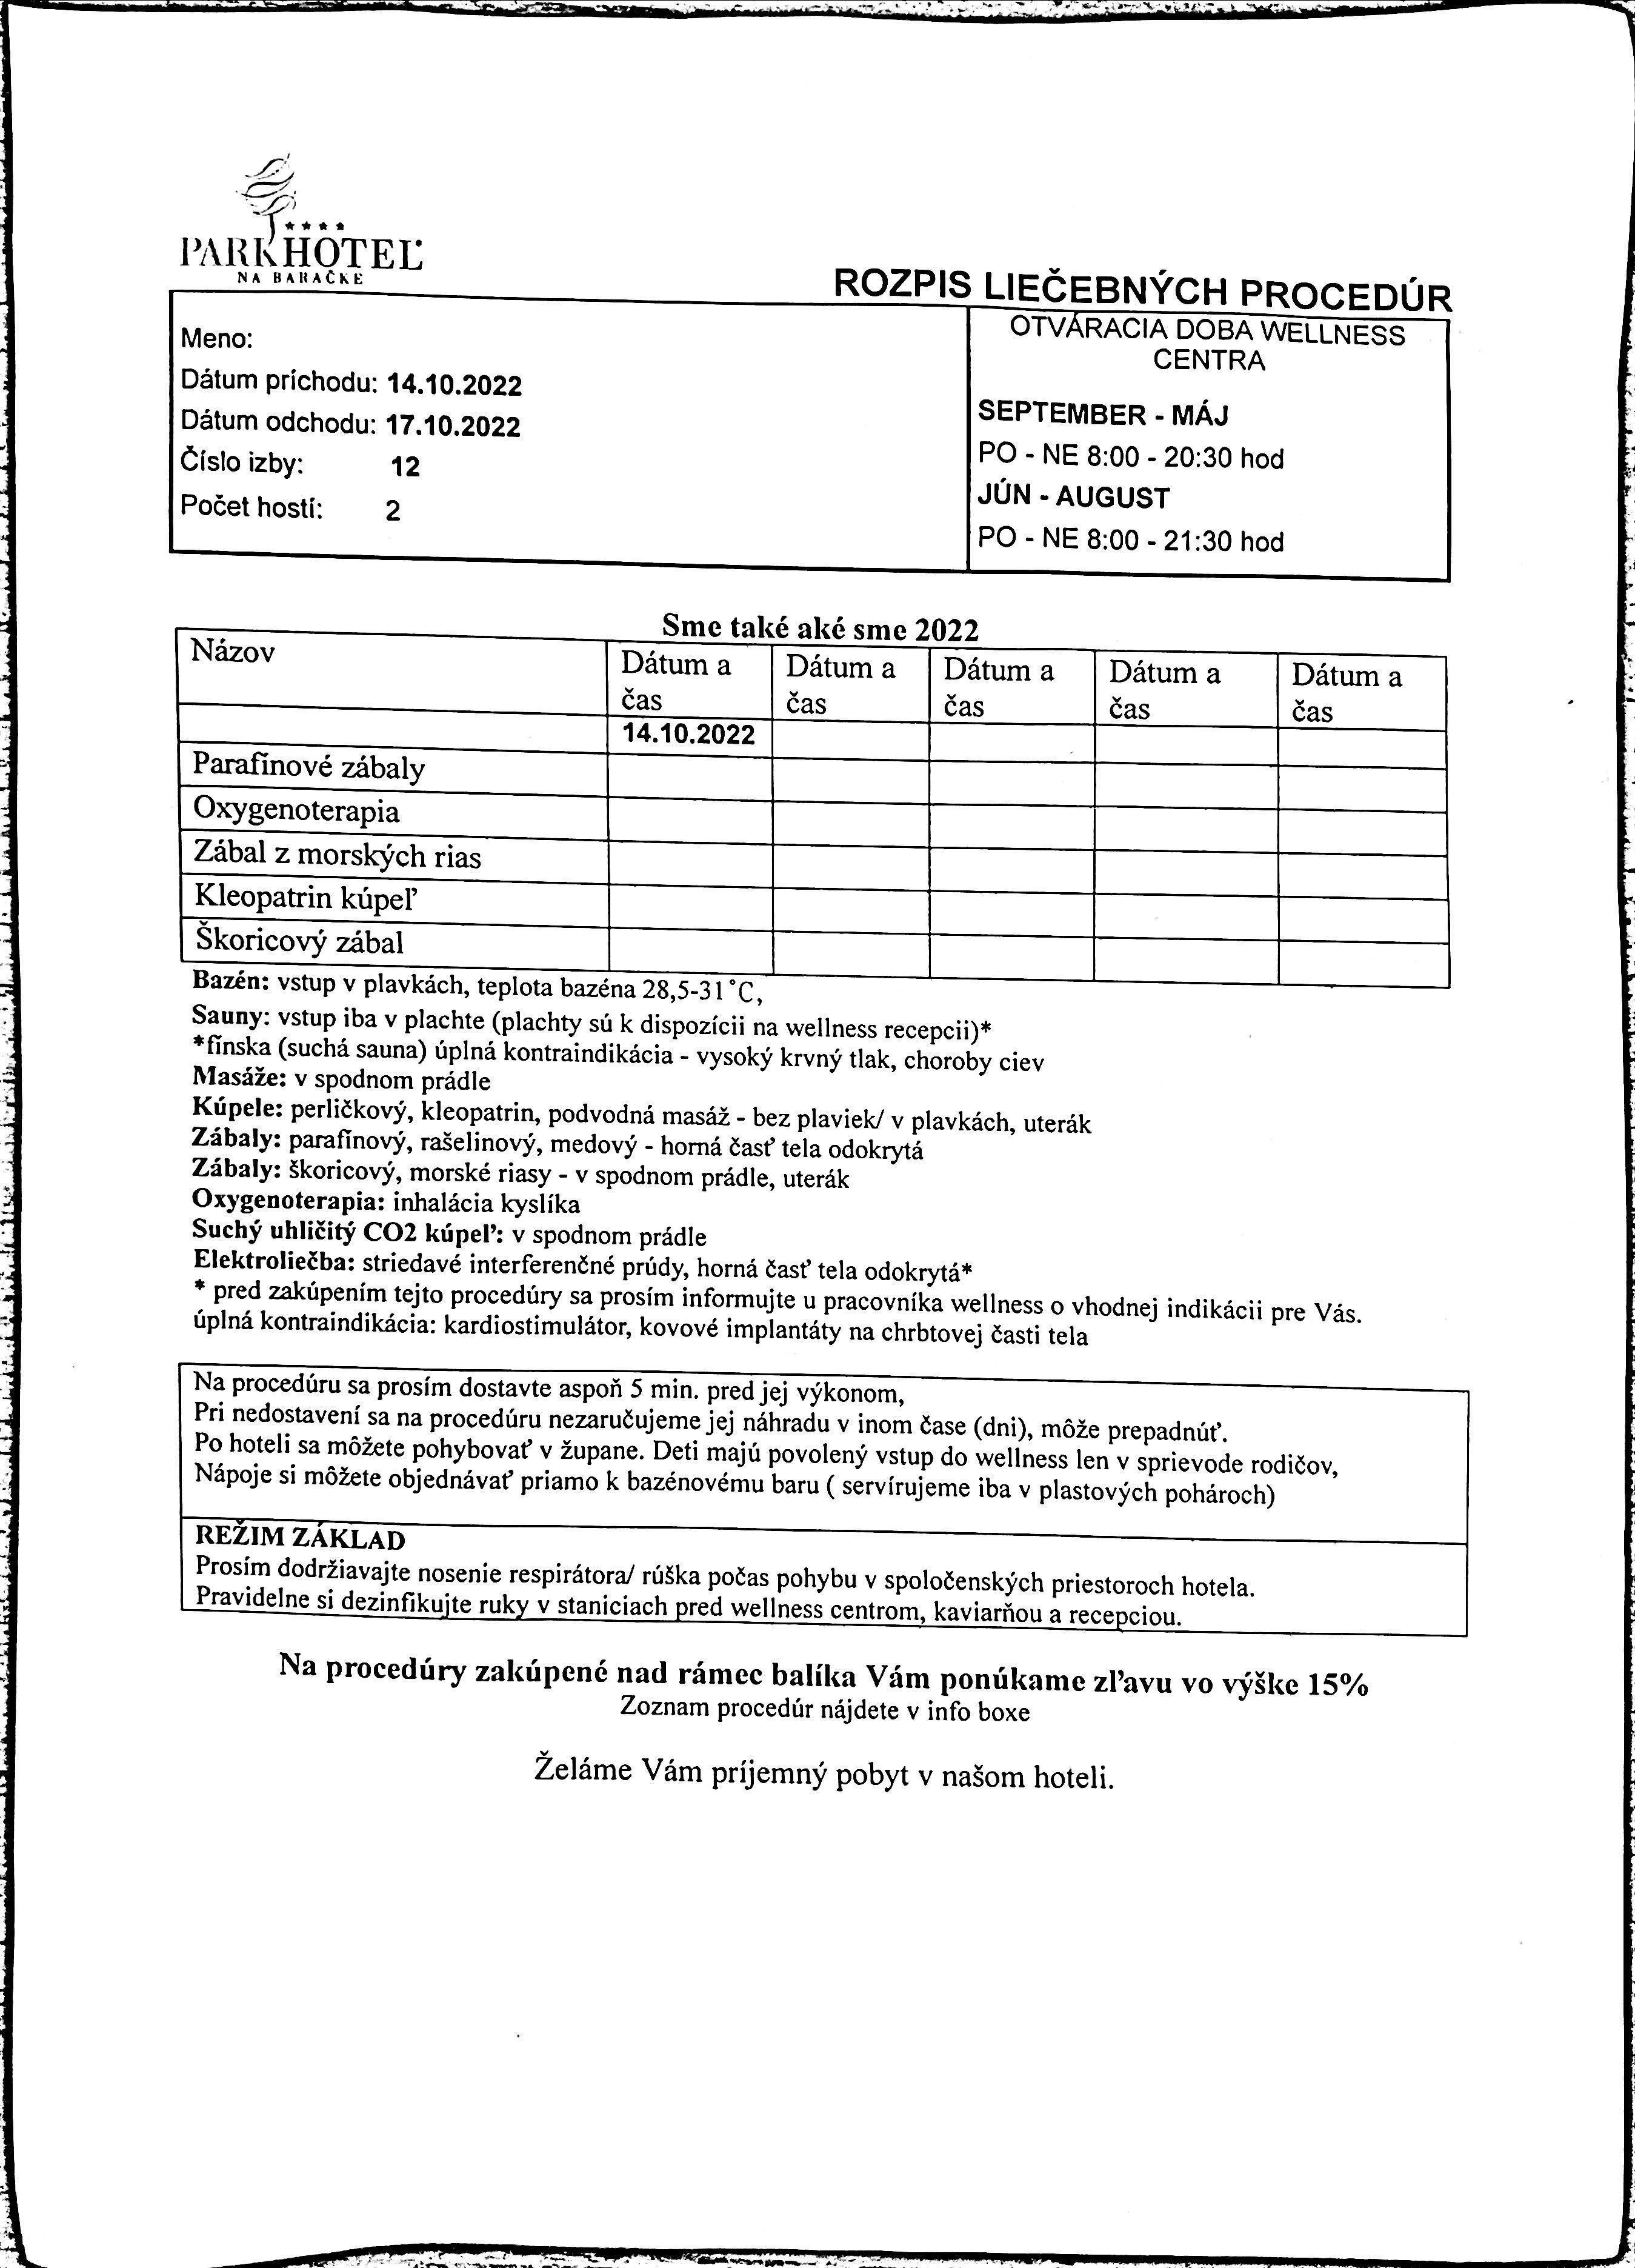
\includegraphics[width=.4\linewidth]{doc/latex/fig/vlado/IMG_9344.jpg}
        \caption{Nabídka služeb}
        \label{fig:parkhotel_wellnes_services}
    \end{subfigure}
    \begin{subfigure}{.5\textwidth}
        \centering
        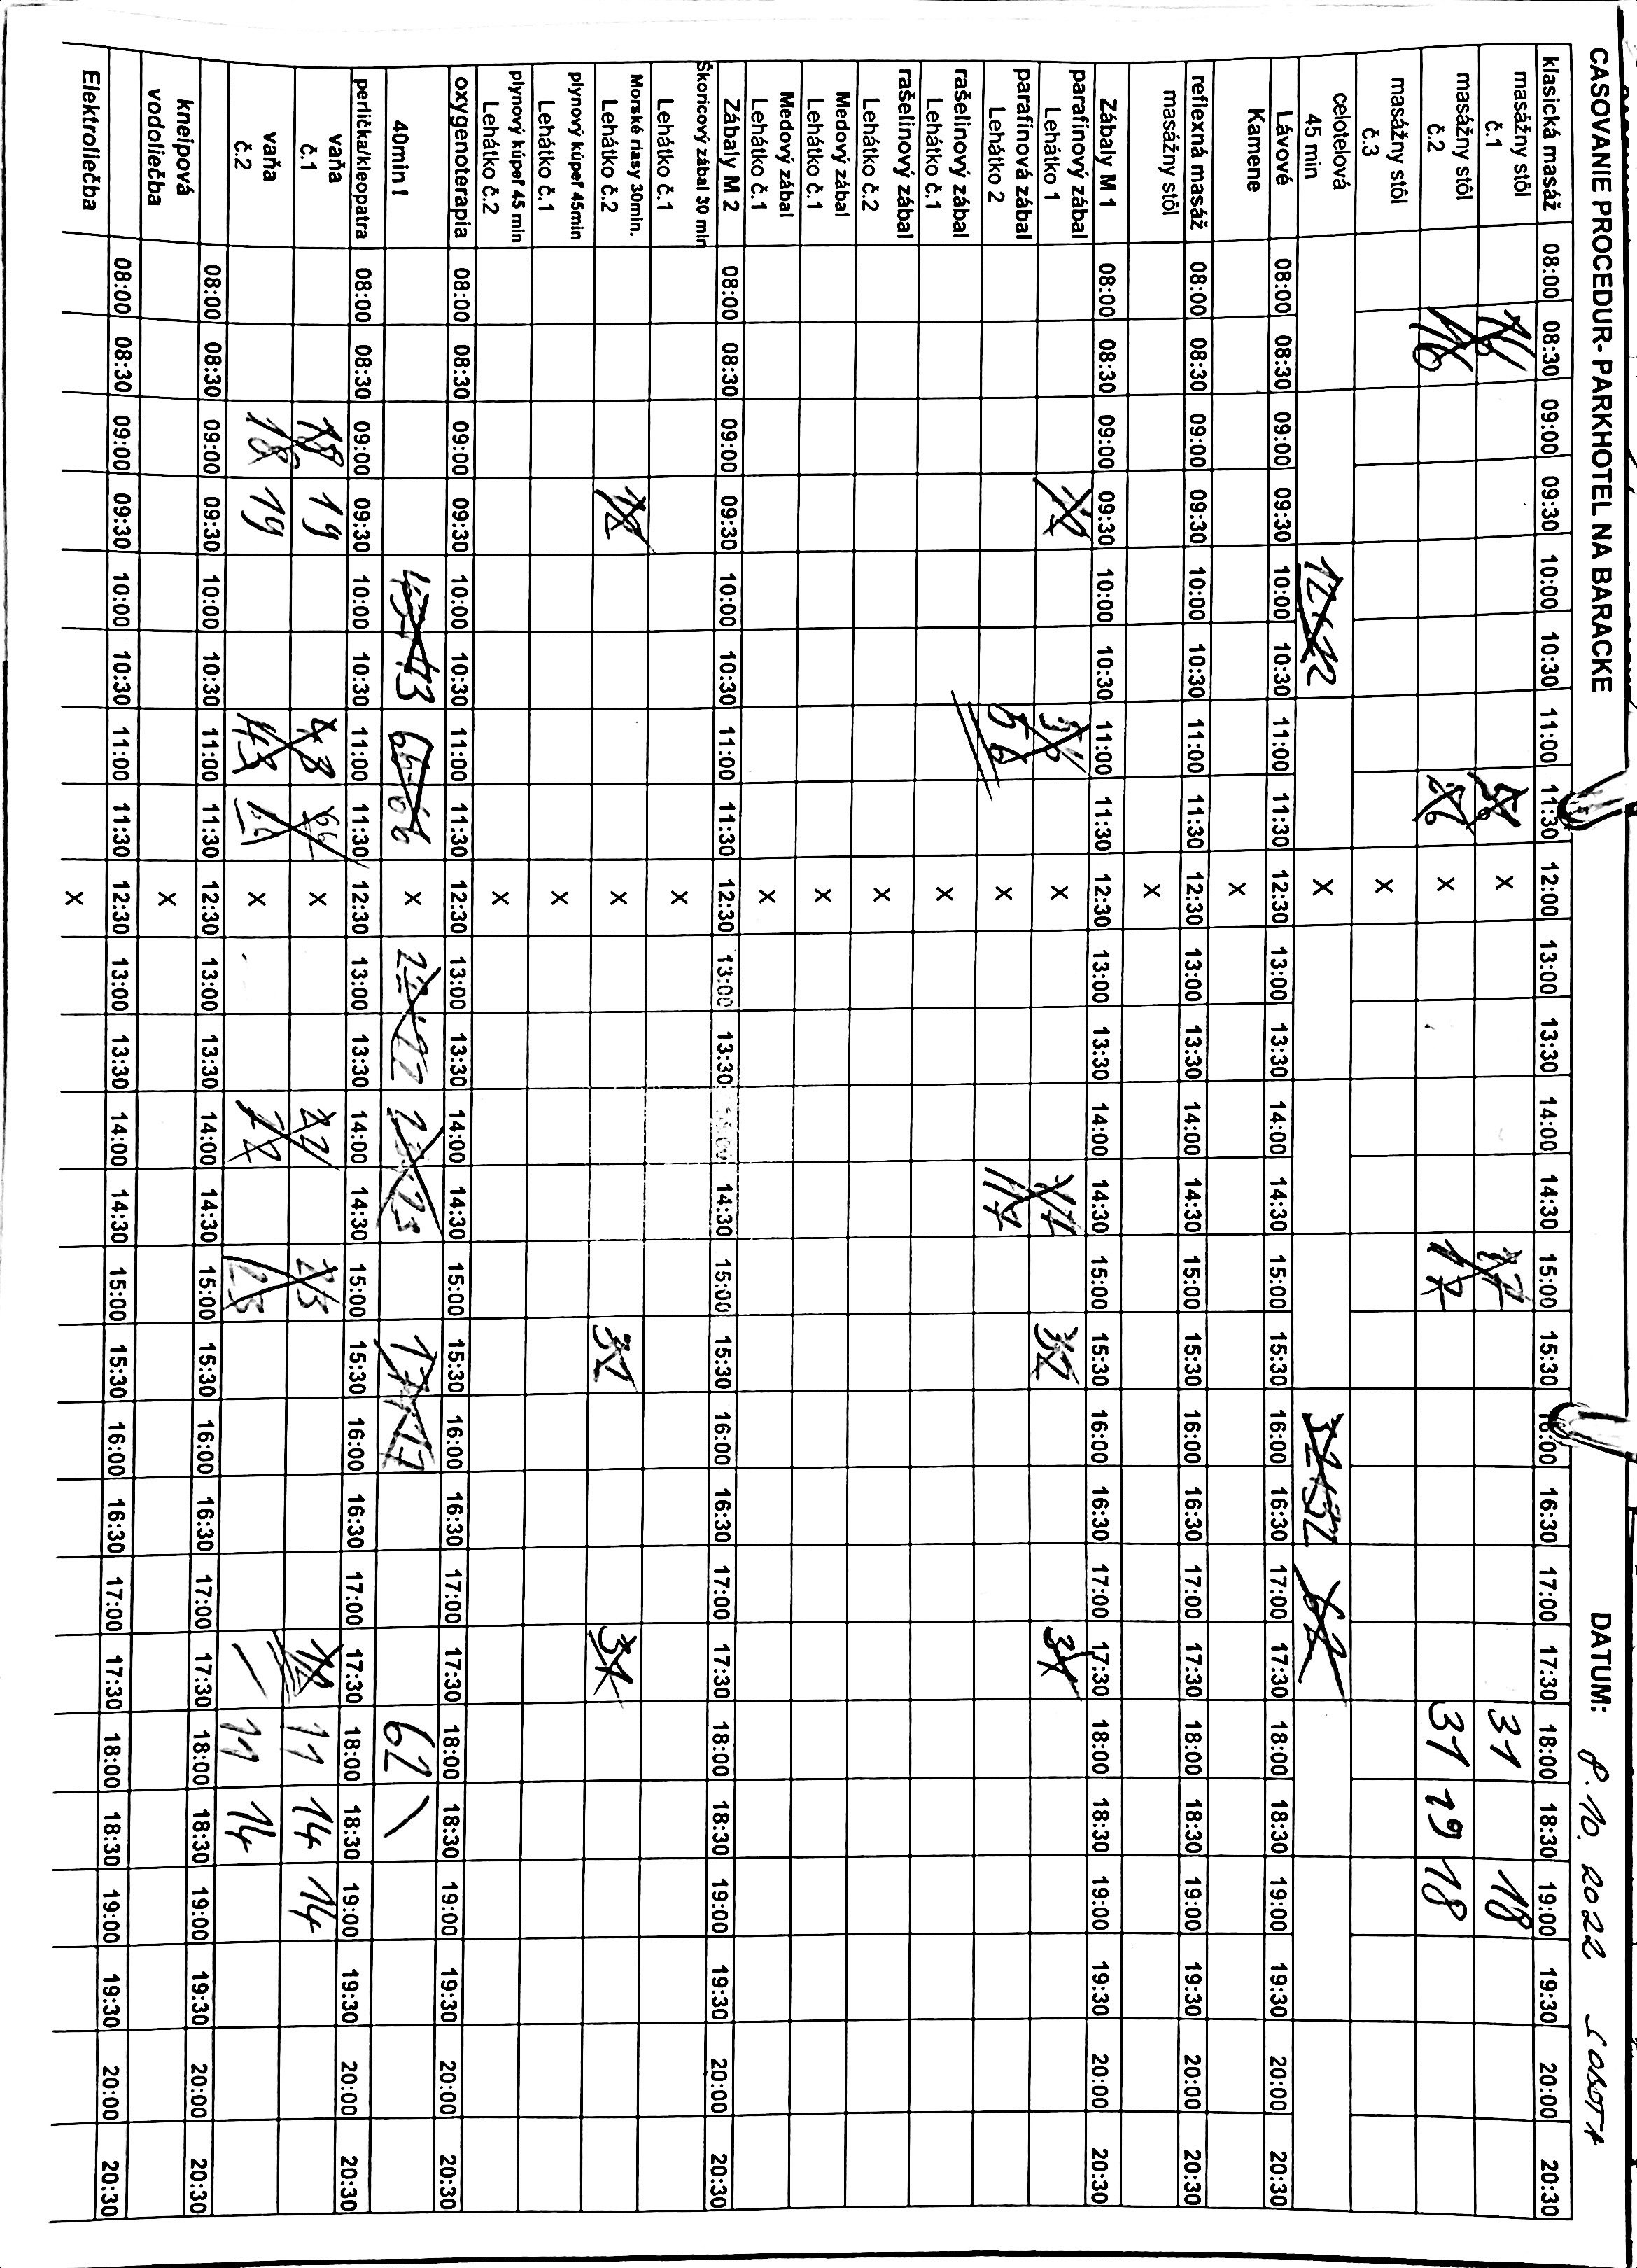
\includegraphics[width=.4\linewidth]{doc/latex/fig/vlado/IMG_9343.jpg}
        \caption{Databáze wellness}
        \label{fig:parkhotel_wellnes_database}
    \end{subfigure}
    \caption{Parkhotel}
    \label{fig:parkhotel}
\end{figure}

\begin{figure}[h]
    \begin{subfigure}{.5\textwidth}
        \centering
        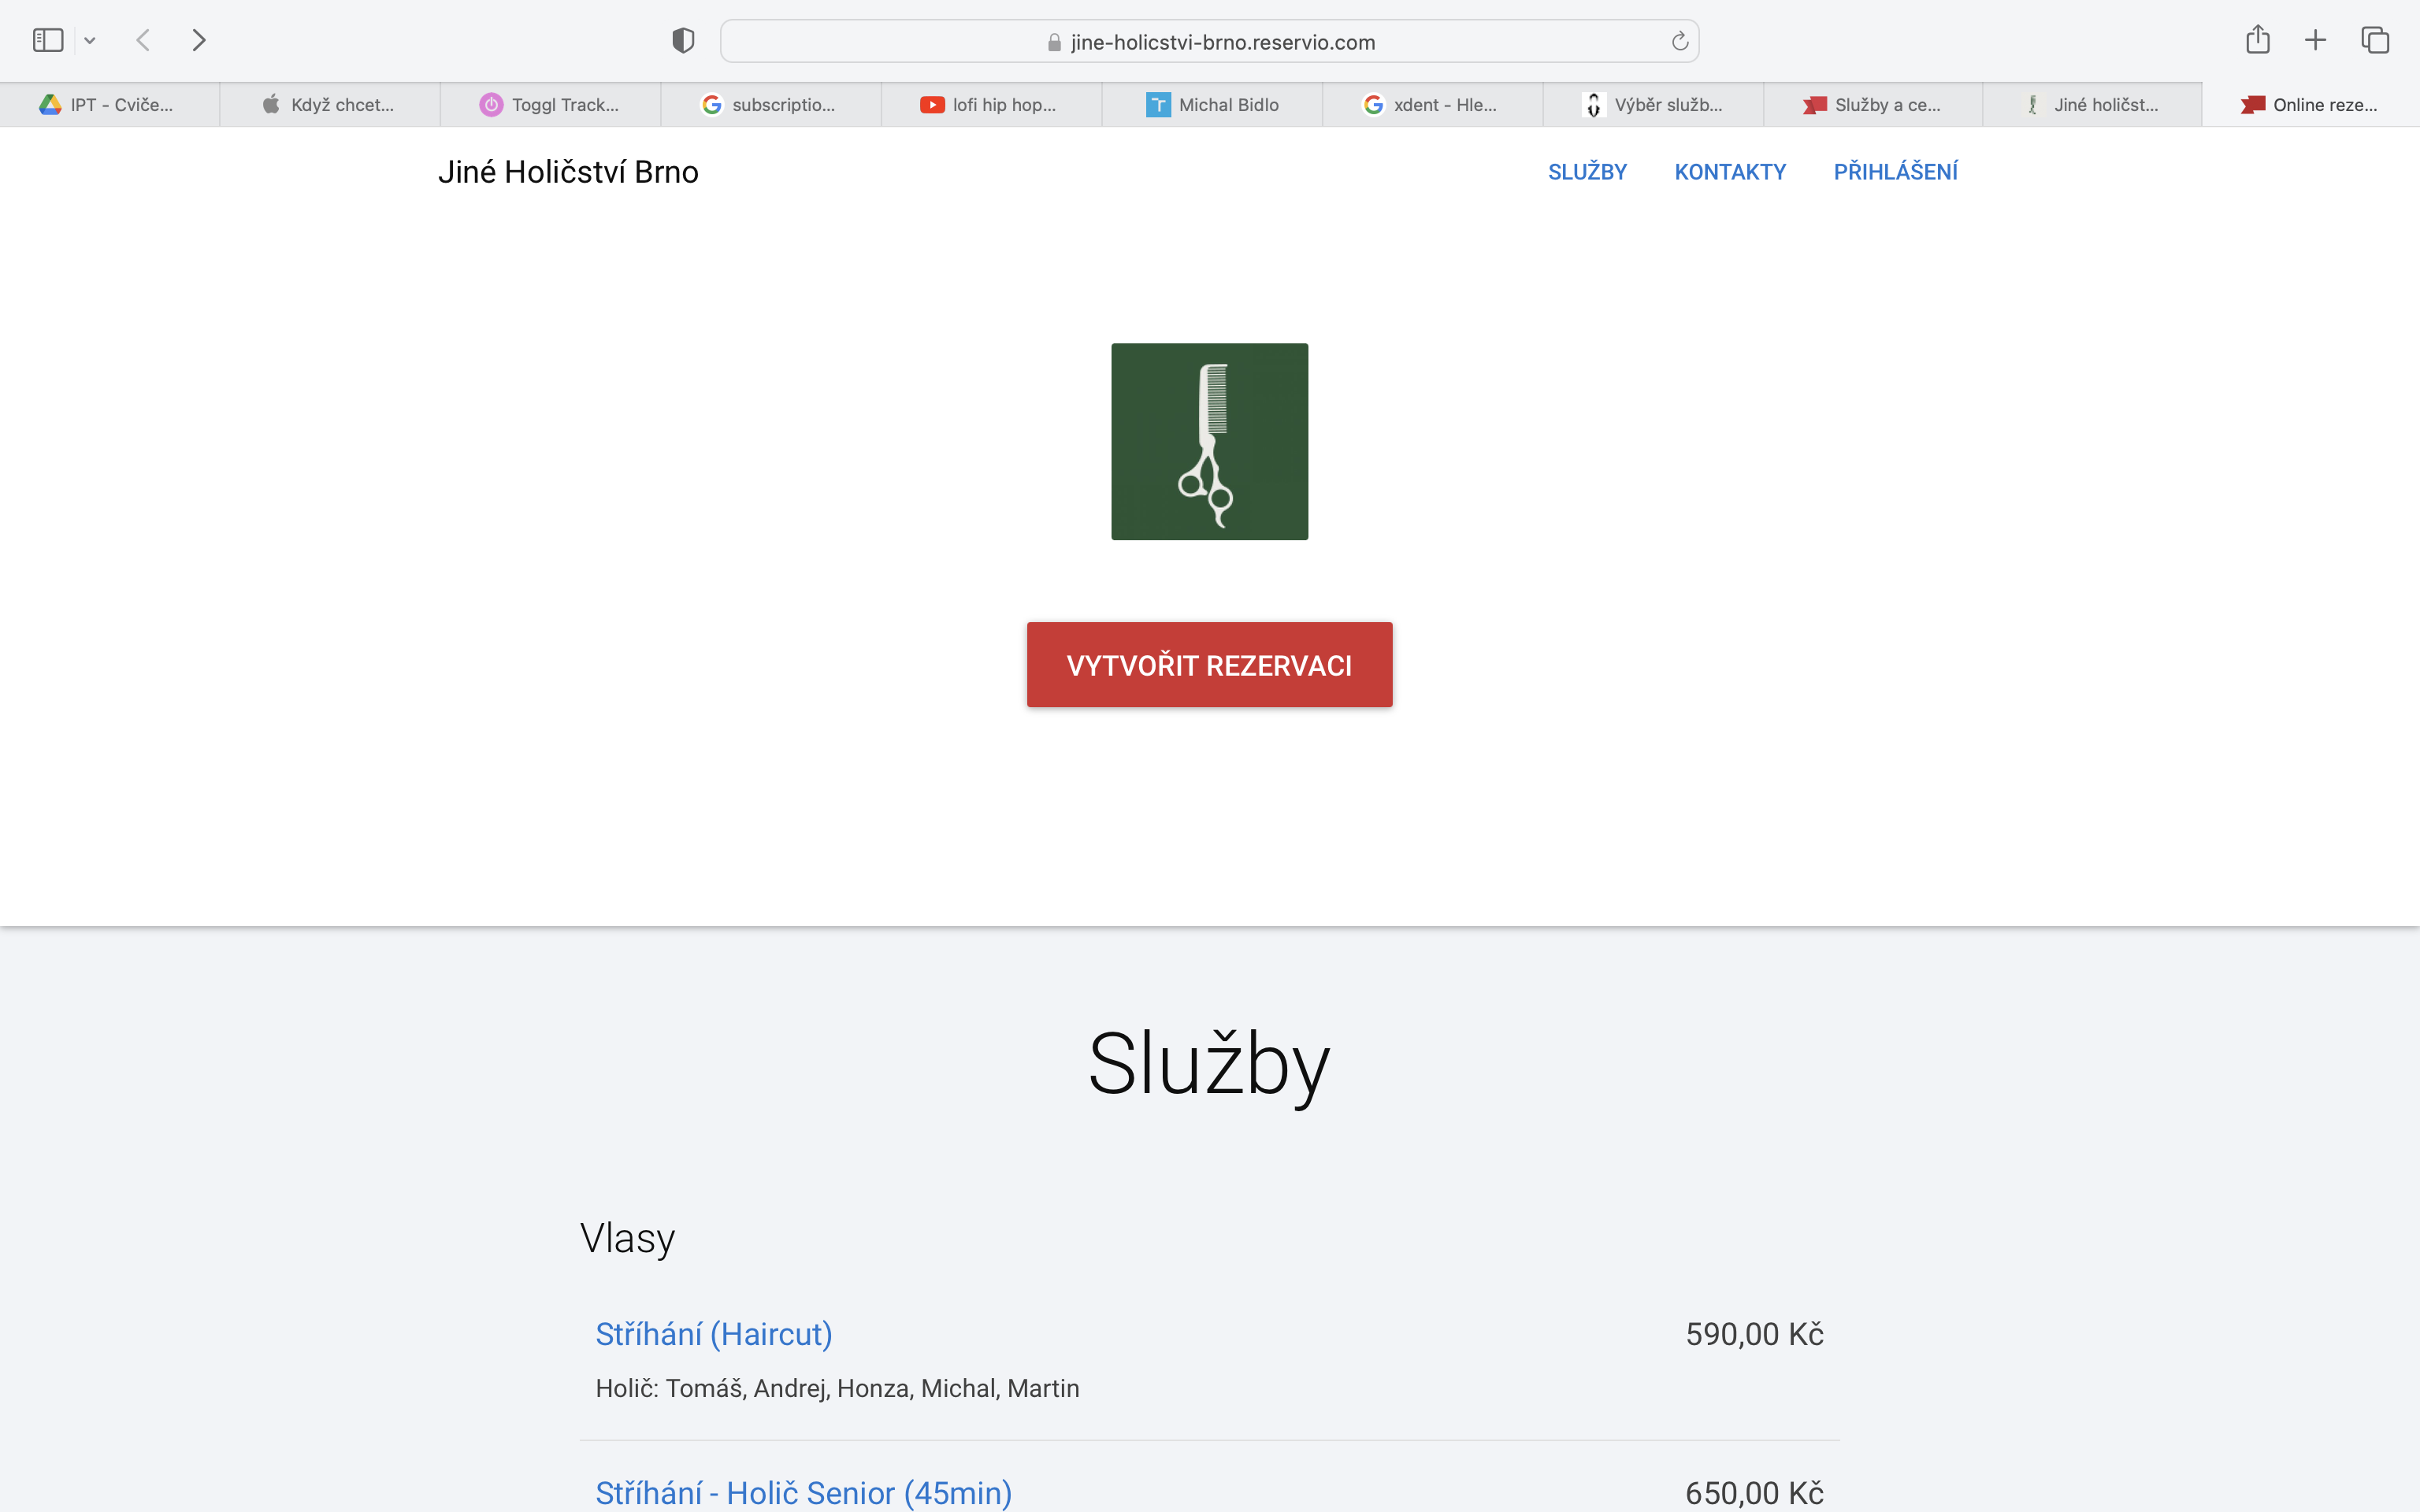
\includegraphics[width=.8\linewidth]{doc/latex/fig/vlado/rezervio_cz.png}
        \caption{Aktuálně používaná webová aplikace}
        \label{fig:current_aplication}
    \end{subfigure}
    \begin{subfigure}{.5\textwidth}
        \centering
        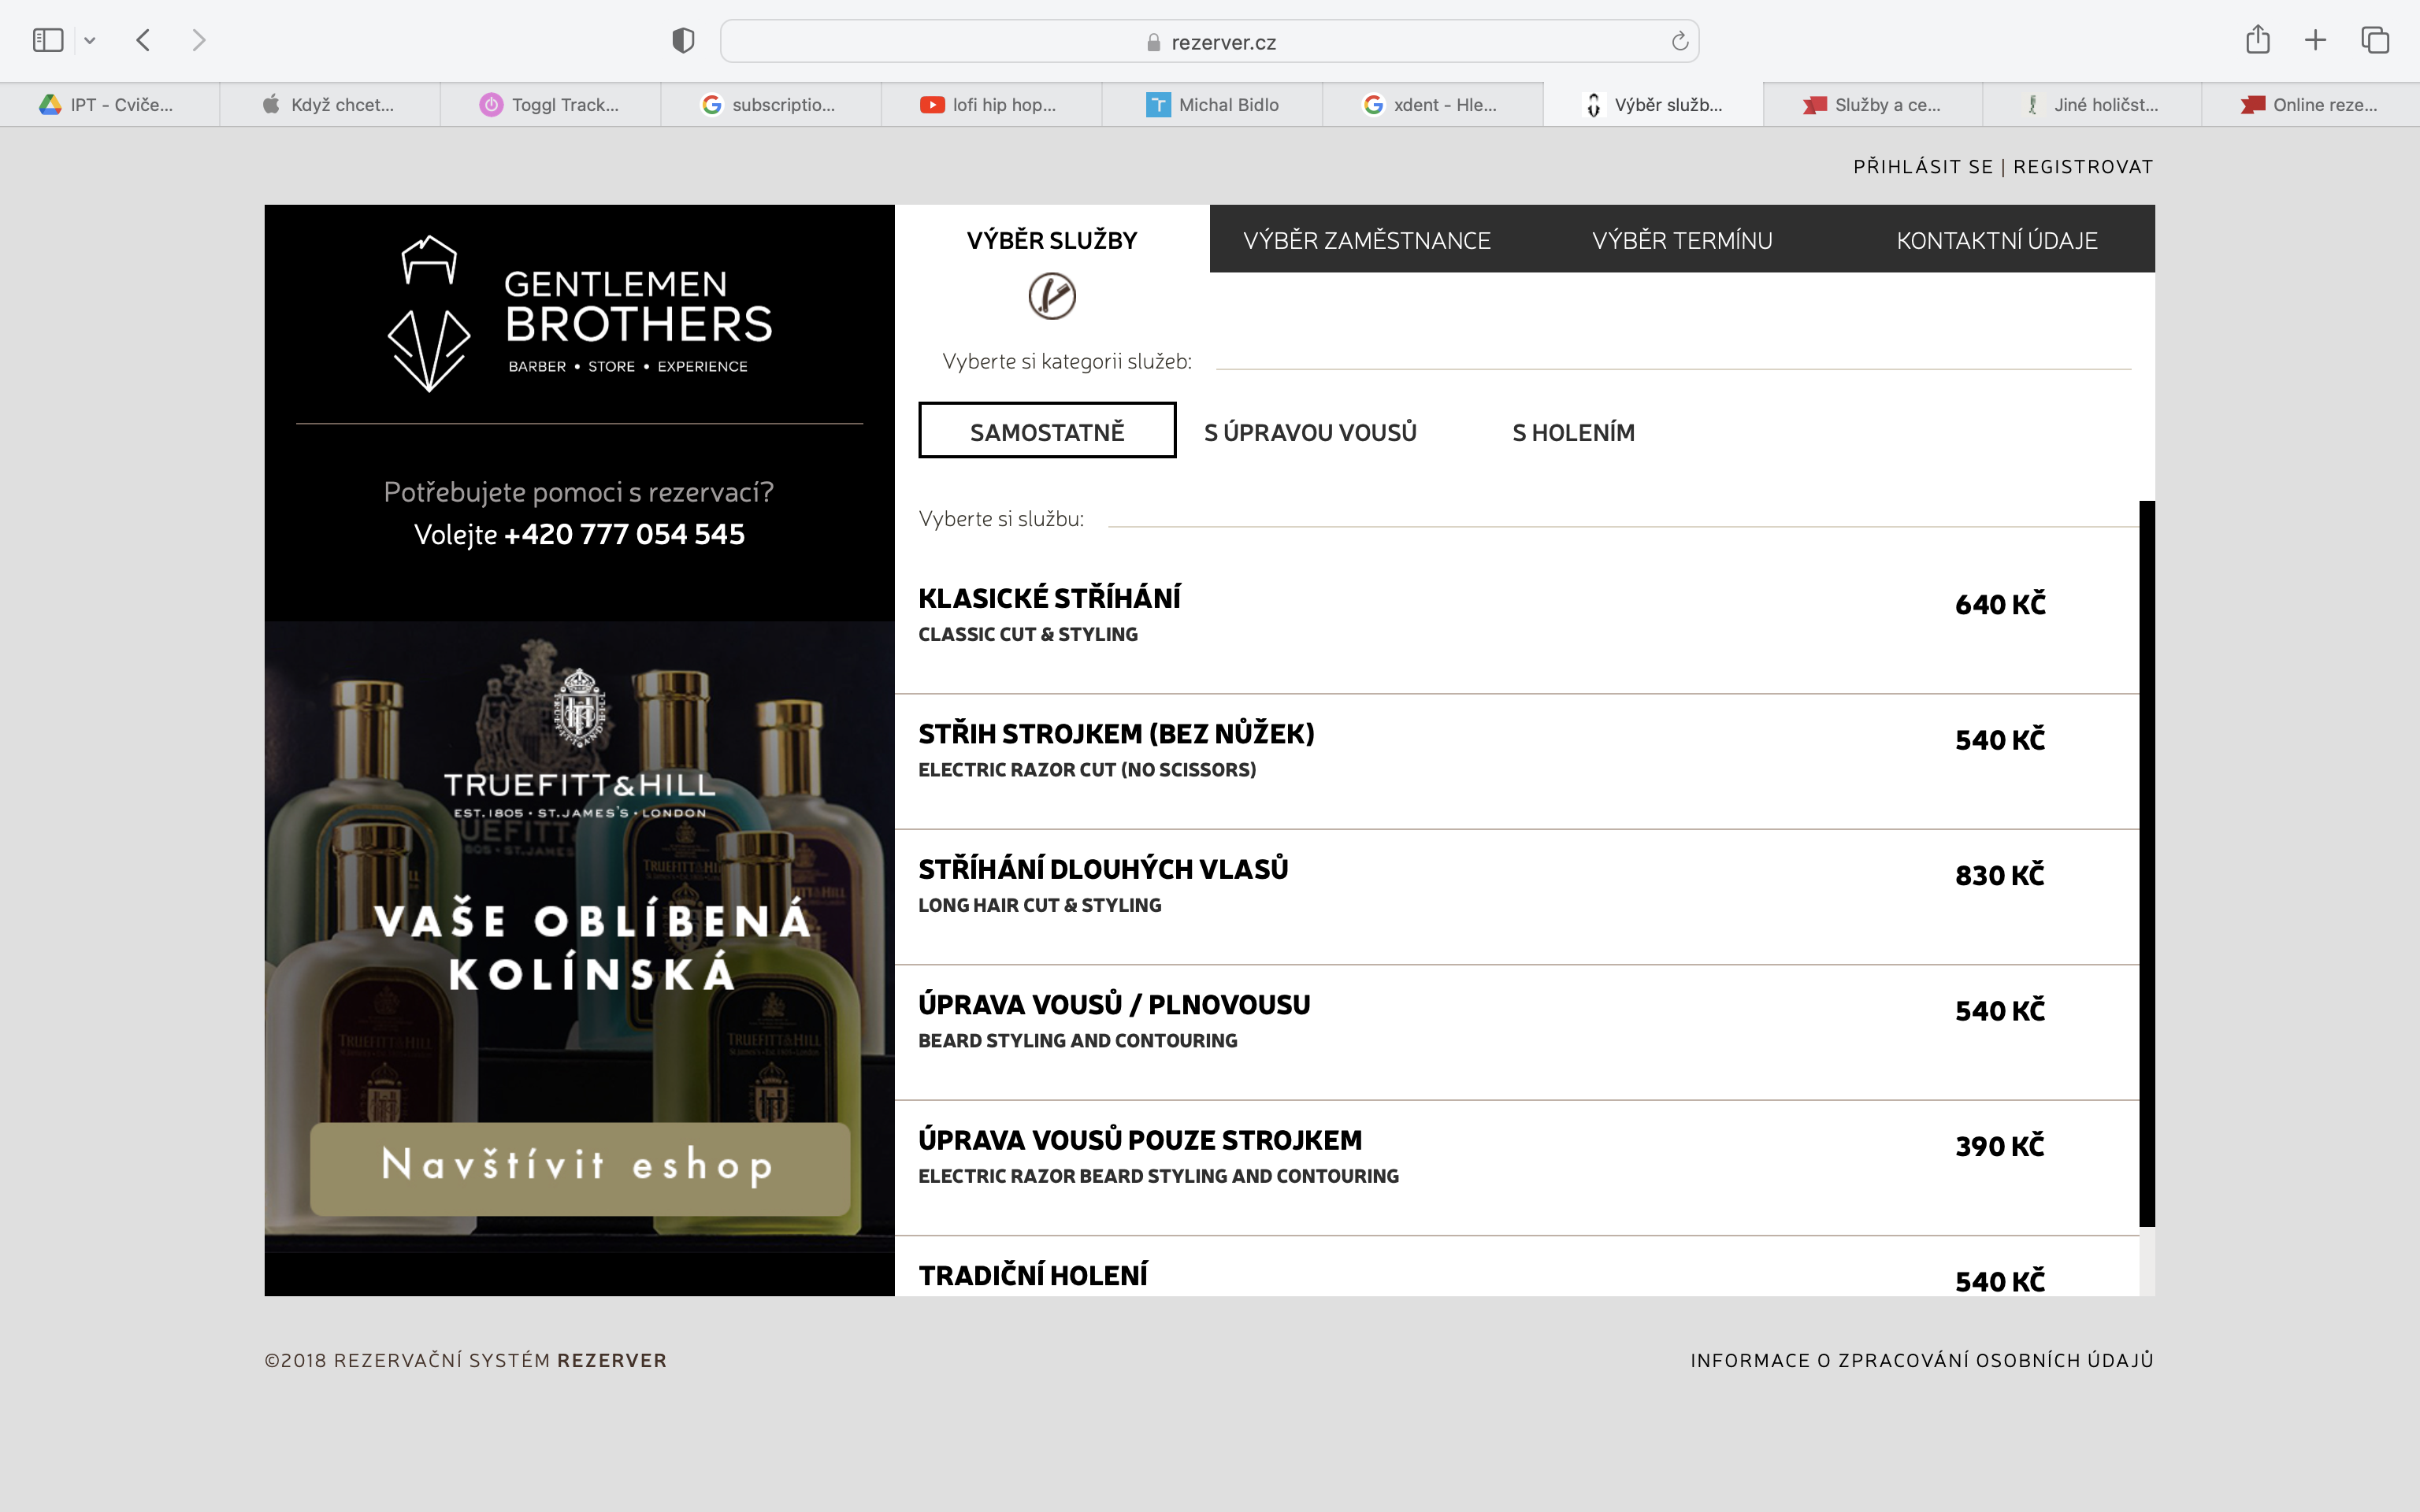
\includegraphics[width=.8\linewidth]{doc/latex/fig/vlado/rezerver_cz.png}
        \caption{Předchozí webová aplikace}
        \label{fig:previous_aplication}
    \end{subfigure}
    \caption{Holičství}
    \label{fig:barber}
    \centering
    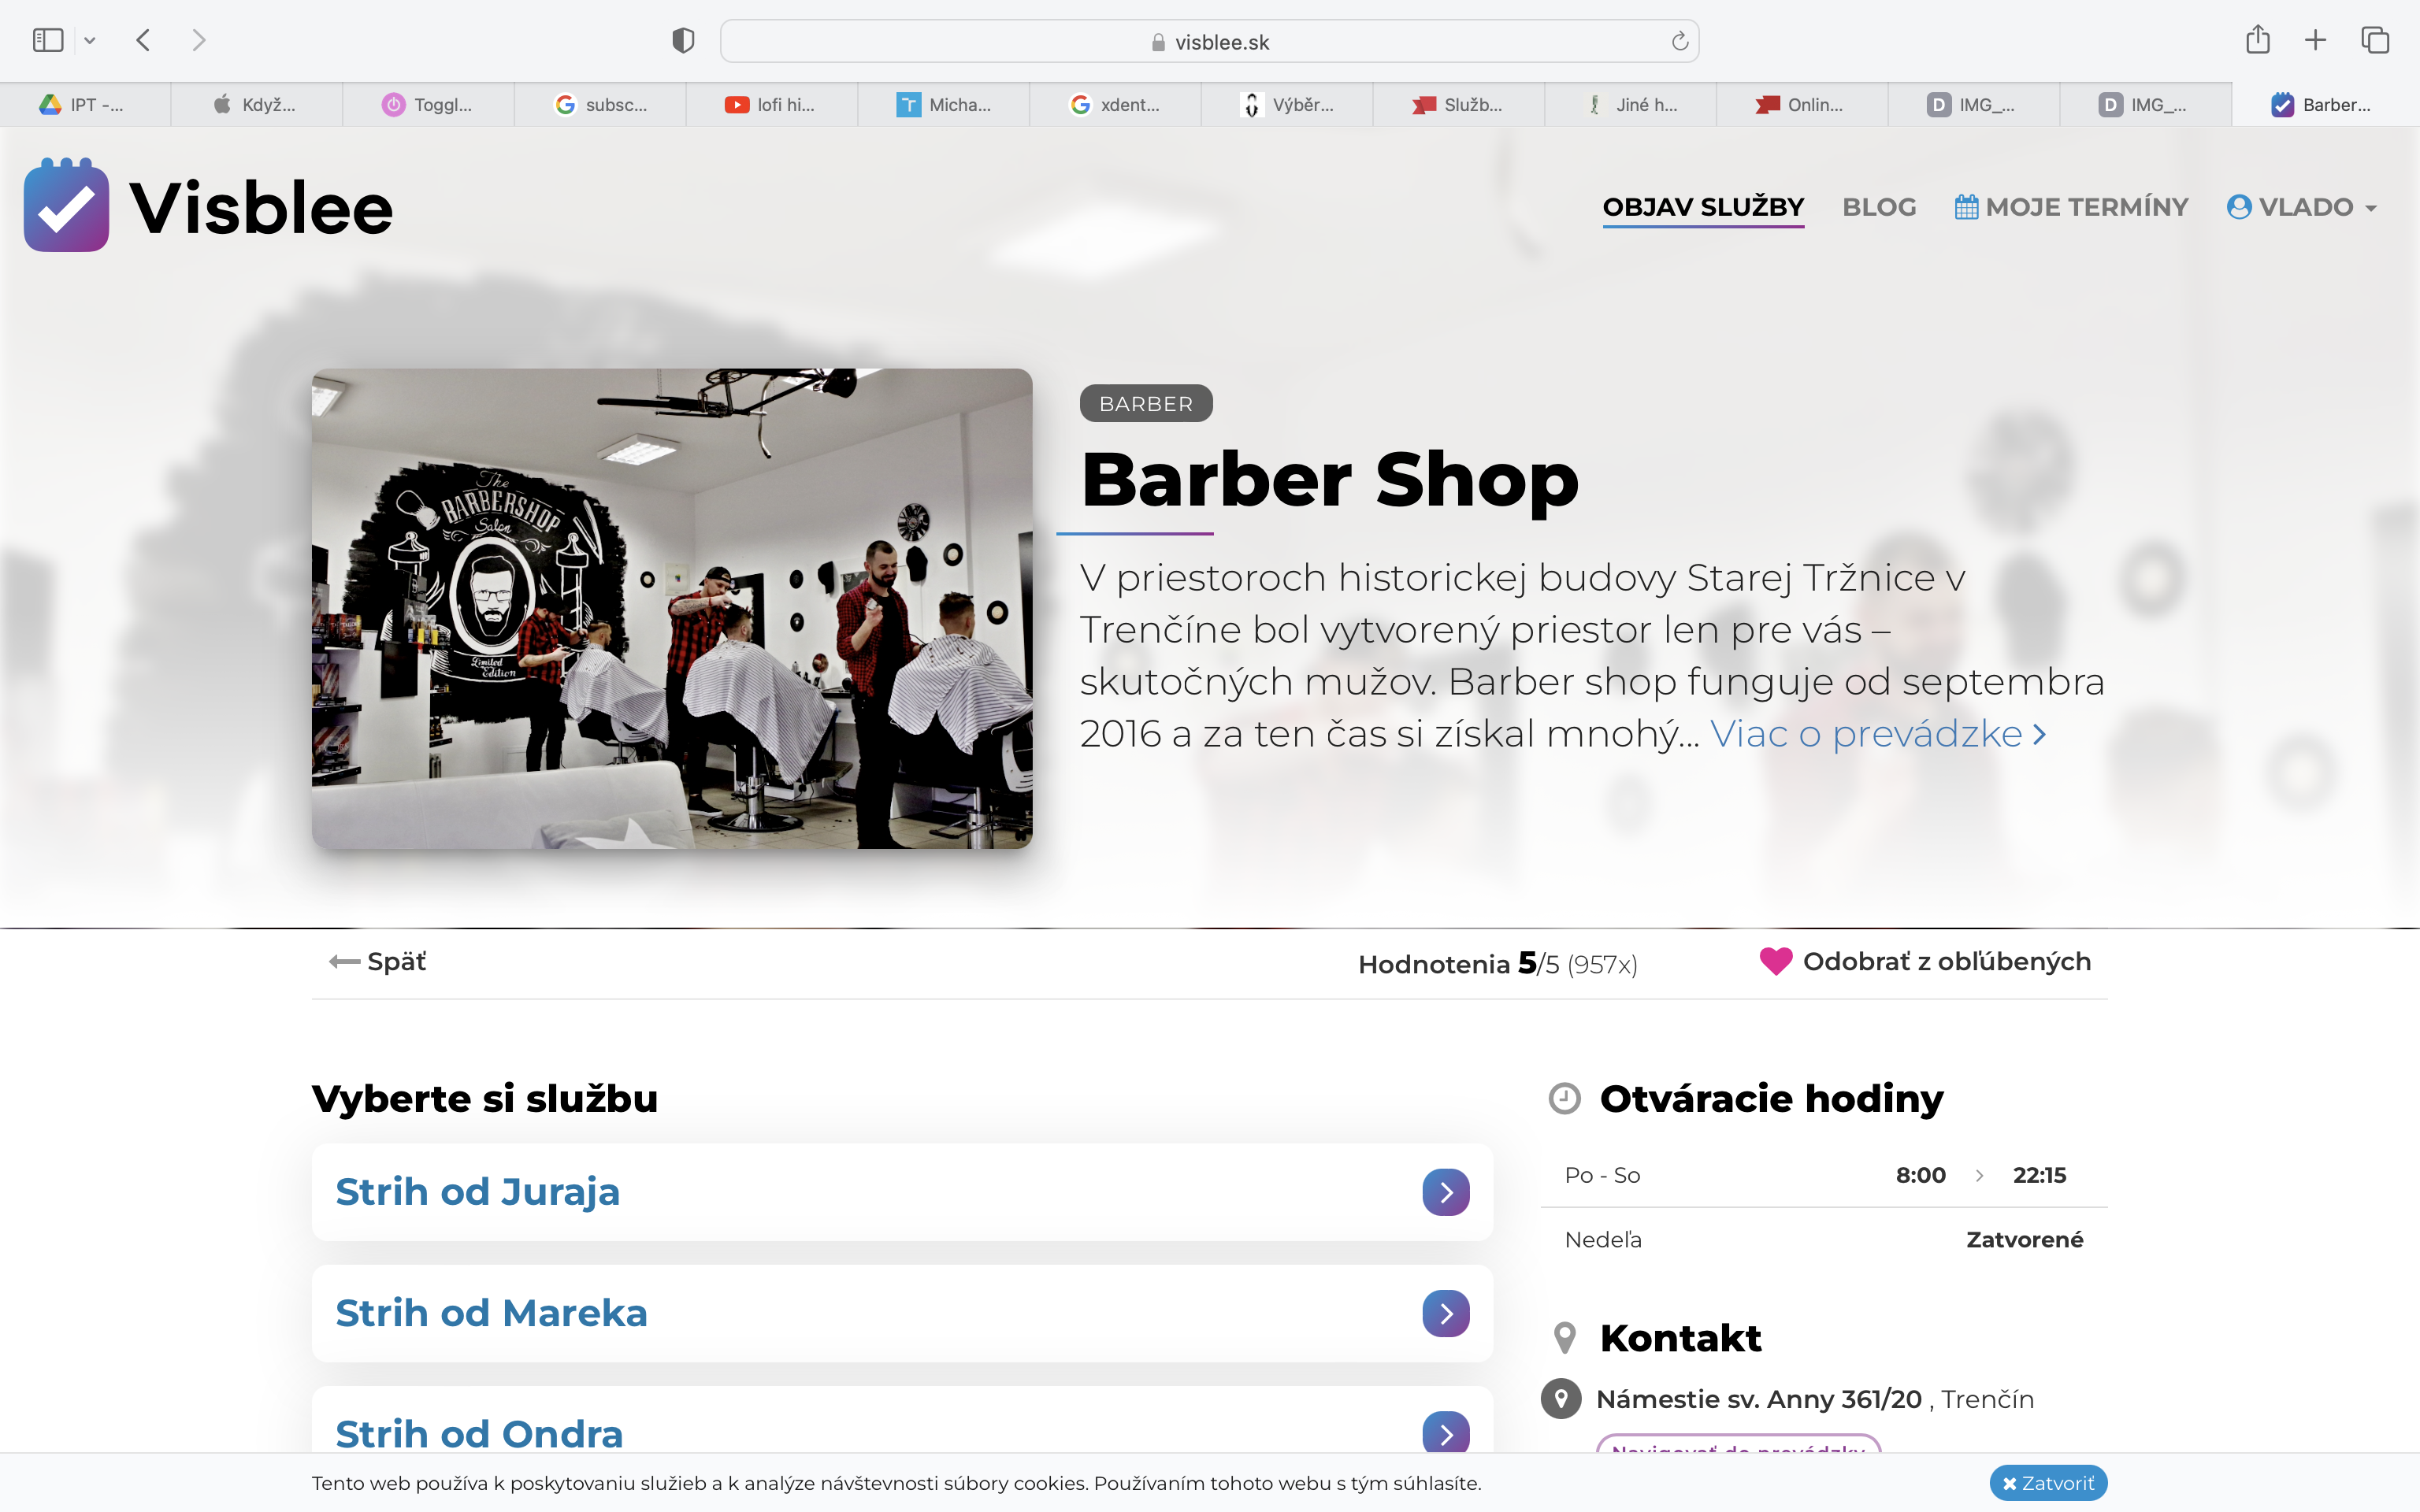
\includegraphics[width=.4\linewidth]{doc/latex/fig/vlado/visblee_sk.png}
    \caption{Aplikace visblee}
    \label{fig:visblee}
\end{figure}
\newpage

\subsubsection*{Navržená sada změn}
Každá z vybraných aplikací a postupů má svoje výhody

\noindent\emph{Jedna aplikace:}
\begin{itemize}
    \item ponechat jednoduchost - dobře zvolit konkrétní postupy rezervací\\ internetových aplikací ponechat v naší
    \item základní funkcionalita - aby bylo možné vytvářet rezervace - potom případně rozšiřovat o další funkcionalitu (statistiky apod.)
    \item vytvořit stylem "plugin" - jedno řešení schopné přepojit se už s internetovou stránkou (možná i v rámci databáze)
    \item Kompatibilita - co nejvíce prohlížečů a zařízení => vytvoření jednoho univerzálního rozšíření pro poskytovatele služeb
\end{itemize}

\subsection{Návrh uživatelského rozhraní, makety rozhraní, testování pomocí maket rozhraní}

\subsubsection{Návrh uživatelského rozhraní}
\noindent\emph{Část projektu v týmu: Návrh rozhraní pro klienty}\\
Rozhraní nově vytvářené aplikace bylo inspirované aplikací resrvio.cz (\ref{fig:current_aplication}). Na~základě průzkumu
mezi uživateli internetové aplikace (konkrétně klienty) jsme se rozhodli použít identický postup rezervace.

\subsubsection{Makety rozhraní}
Maketa rozhraní ponechá jednoduchost a intuitivnost aplikace reservio.cz \ref{fig:current_aplication}. Prvotní prvek (tlačítko)
bude "připojený" k internetové stránce. Zákazník se přes něj bude moct dostat přes jednotlivé kroky rezervace.  \\
To konkrétně:\\
\begin{itemize}
    \item[1] Výběr služby, nejprve pomocí primární služby a potom výběr jednotlivých podsekcí služby
    \item[2] Výběr zaměstnance
    \item[3] Výběr data a času
    \item[4] Doplnění údajů (neplatí pro přihlášeného uživatele)
    \item[5] Potvrzení o vytvoření rezervací modulárním oknem a přesměrování na původní stránky poskytovatele služeb
\end{itemize}


\newpage
\begin{figure}[h]
    \centering
    \includegraphics[width=1.4\textwidth, angle=270]{doc/latex/fig/vlado/Reservation_client_part-1.pdf}
    \caption{Navržená maketa}
    \label{fig:mokcup}
\end{figure}
\newpage

\subsubsection{Testování pomocí maket rozhraní}
Testování rozhraní proběhlo v aplikaci Figma na spolužácích v týmu a mých známých kteří mi
pomohli napravit nedostatky. Věřím, že s jejich pomocí byla vytvořená co nejlepší maketa.

\newpage

    \section{Samostatná práce člena týmu\ --\ Ondřej Fojt}
\label{sec:individual_work_ondra}

\subsection{Výběr tématu, popis provedeného průzkumu s uživatelem, analýza uživatelských potřeb a klíčových problémů, navržená sada změn}

\subsubsection*{Výběr tématu}

{\large Můj návrh:}

Checklist/TODO manažer na hlídání deadline pro kohokoliv, kdo dělá více projektů zároveň.


{\noindent \large Vybraný návrh v týmu:}

Medicínský systém pro přihlašování klientů na procedury/sezení/vyšetření. Zaměření především na přihlašování klientů a zobrazení těchto přihlášek

\subsubsection*{Provedený průzkum}

{ \noindent \large Technická podpora zubní ordinace:}

U přihlašování pacient sám neví na jak dlouhou dobu se má objednat. Většinou pacienti spíše volají/píší emaily, protože si nejsou jistý jak se objednat. Objednat se by mělo zabrat co nejméně kroků

{\noindent \large Pacient co se chce přihlásit:}

I když je tlačítko pro odeslání/pokračování velké a má velký kontrast pokud je umístěno úplně ve spodku obrazovky, tak si ho dost lidí nemusí rychle všimnout. V naléhavém případě může být online přihlašování restriktivní (když někoho bolí zub, tak asi nebude chtít čekat 2 týdny)

{\noindent \large Doktor provádějící vstupní prohlídky}

Dětské rehabilitační oddělení
\begin{itemize}
    \item  K lékařům na prohlídku se neobjednává. Je důležité, aby si lékaři mohli na pacienty vyčlenit čas, co nejdříve. Mají frontu, kde pacienti případně počkají. Náhled do fronty vidí doktoři i skrze informační systém nemocnice, kde mohou vidět některé zprávy o pacientech, číslo pojišťovny, zaměstnavatele atp. Lékaři dávají i termíny, kdy mají přijít na kontrolu bez nutnosti registrace.
    \item  V ošetřovně je jeden telefon, který berou doktoři. Přesto, že se neobjednává, tak 20\% lidí zavolá, aby se ujistili či objednali. Případy, které lze odložit se snaží doktoři přesunout na místa, kdy chodí málo lidí. 
    \item  Na jednotlivé rehabilitační procedury lékaři pevně objednávají pacienty v rozmezí ambulantní doby. Oddělení poskytuje různé služby jako jsou např. laser, magnet a fyziocvičení. 
    \item  Doktoři mají kalendář do kterého si dělají čárky, které znázorňují obsazenost procedur. Čárka značí pacienta. Do objednávkových sešitů se zaznamená jméno a kontakt v případě nemoci doktora. V takovém případě se každému zavolá a přesune se ho. Každá procedura má svojí obsazenost. Např. je dobré aby magnet byl značně obsazený, když už je zapnutý, ale aby i bylo možné na poslední chvíli někoho přidat. Magnet má doporučenou obsazenost 90\%.
    \item  Nevýhodou je, že již není k dispozici procentuální obsazenost, že si nelze lehce vyhledat termíny pacienta. Nelze zjistit z domova, zda mám dnes volněji. Je třeba zadat údaje dvakrát - do kalendáře a do papírku potvrzující objednání. Nelze zjistit z domova, zda mám dnes volněji. 
    \item  Výhodou systému je zažitost a netěžká obsluha. Netřeba zapínat tablet či počítač.
    \item  Potřeby uživatele, lékařů a fyzioterapeutů, jsou evidovat pacienty a případně je zarezervovat, znát volné termíny, možnost zkontrolovat, kdo přijde. Je potřeba evidovat čísla pro pojišťovnu pro vyplacení peněz.
\end{itemize}

\subsubsection*{Analýza potřeb a klíčových problémů}

U některých registrací není dopředu známý čas. Mnoho lékařů používá pouhé kalendáře (online nebo papírové) -> jakou motivaci mají k používání našeho systému? Přihlašování akutních/speciálních případů v rozumném čase.

První vyšetření u lékaře se nedá vě většině případů naplánovat. Doktorovi se hodí vidět zaplněnost jednotlivých služeb, aby se mohl rozhodnout kam pacienta objedná, pokud může být rehabilitován více různými procedurami.
Fyzioterapeutovi by se spíše hodilo vidět jména a kontakty pacientů v rámci registrací a aby je mohli sami registrovat na termín, který není příliš zaplněný.


\subsubsection*{Navržená sada změn}
\noindent\emph{Návrh I.}

Pacient by měl možnost vybrat více termínů, které se mu hodí a po určité době mu bude sděleno, kdy má přijít.

\noindent\emph{Návrh II.}

Pro akutní případy umožnit zkrácení délky okna termínu, aby měli možnost přijít co možná nejdříve.

\noindent\emph{Návrh III.}

Při výběru v rámci přihlašovacího formuláře rovnou zobrazit další krok místo nutnosti klikat na tlačítko další.

%\newpage
\subsection{Popis současného řešení\ --\ jaké nástroje uživatel používá, \\
popř. obrázky/screenshoty současného řešení/reálné situace}

\noindent\emph{Poznámky v kalendáři/online dokumentu/e-mailech} 
\begin{itemize}
    \item[+] Není potřeba získat a naučit se nový systém
    \item[--] Nestrukturované
    \item[--] náročné na vyhledávání určitých přihlášek
    \item[--] potřebná komunikace pro přihlášení ze strany zaměstnance
\end{itemize}

\noindent\emph{XDENT viz \ref{fig:Ondra_xdent_admin}.}
\begin{itemize}
    \item[+] Umožňuje online přihlašování, chat s pacientem, upomínky...
    \item[+/--] Specializováno pro zubní ordinace
    \item[--] Měsíční poplatky za licenci a služby 
\end{itemize}

\begin{figure}[htbp]
    \centering
    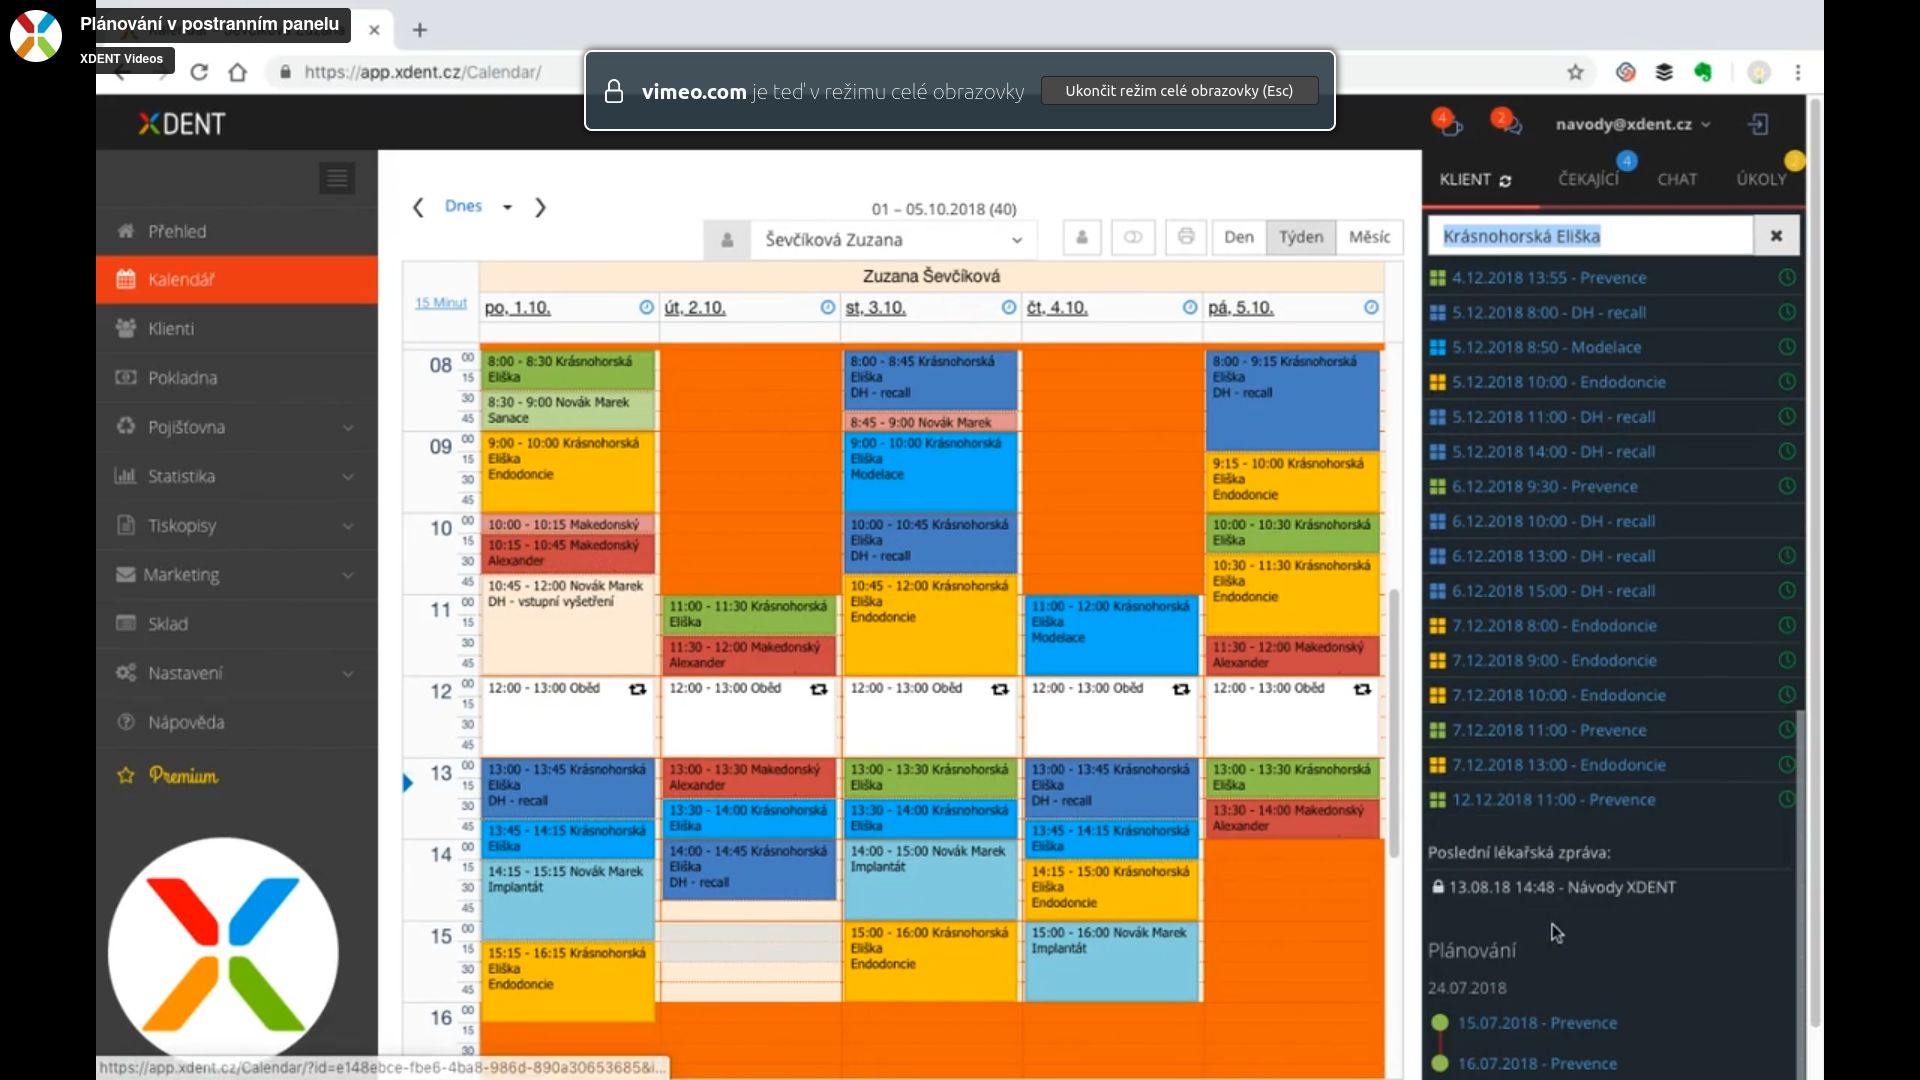
\includegraphics[width = \textwidth]{doc/latex/fig/ondra/xdent-admin.png}
    \caption{XDENT: Pohled přihlášeného zaměstnance/administrátora}
    \label{fig:Ondra_xdent_admin}
\end{figure}

\newpage

\noindent\emph{Týmuj}
\begin{itemize}
    \item[+] Každý přihlášený může uvést k dané událost, zda se zúčastní nebo ne
    \item[--] není přímo z lékařství -> vytvářet termíny může každý
\end{itemize}

\subsection{Návrh uživatelského rozhraní, makety rozhraní, testování pomocí maket rozhraní}

\emph{Část projektu v týmu: Návrh rozhraní pro zaměstnance}

\subsubsection*{Návrh}

\begin{itemize}
    \item Lze najít nejbližší události
    \item Lze Zobrazit události ostatních zaměstnanců
    \item Jednoduché zobrazení podrobností o události
    \item Přidání/změny událostí pouze po potvrzení interakcí
    \item Zaměstnanec(dle vnitřní politiky) může vyhledávat/měnit časy, kdy může poskytovat jednotlivé služby
\end{itemize}

\subsubsection*{Maketa}

{\noindent\Large Popis makety}

Hlavní stránka viz \ref{fig:Ondra_figma_mainpage} slouží pro rychlé zorientování v nadcházejících\\ událostech pro daného zaměstnance. 
Umožňuje změnit pohled, což znamená ukázat události, rozvrh, jiného zaměstnance. Tohle se může hodit například pokud potřebuji vědět, kde ve který čas někoho můžu najít.
Dále se na stránce nachází seznam několika nejbližších tedy nadcházejících událostí. Zobrazují se zde služby, které zaměstnanec poskytuje a také vnitřní organizační záležitosti firmy/organizace.
Na spodní straně stránky se nachází kalendář událostí, pro lepší orientaci v termínech událostí. V něm lze vyhledávat, tisknout ho a v případě nutnosti také upravovat.
Úprava událostí by měla být možná pouze daným zaměstnancem nebo jeho nadřízenými.

Vyskakovací okno ukázané na obrázku \ref{fig:Ondra_figma_event_detail} se zobrazí po kliknutí na událost.
Okno obsahuje název události, datum a čas, místo konání, zodpovědnou osobu(v případě služeb bude obsahovat jméno zaměstnance 
na jehož pohled se například díváme, ale nemusí tomu tak vždy být), jednotlivé účastníky, u kterých bude možnost otevřít okno s kontaktem na danou osobu, 
a nakonec popis události, který dle události může vyplňovat zaměstnanec nebo klient, který se na událost přihlásil.
Ve vyskakovacím okně nelze nic měnit pokud není zapnutý režim pro úpravu událostí.

Protože každý zaměstnanec může poskytovat různé služby a také se můžou dramaticky 
lišit pracovní doby zaměstnanců je k dispozici stránka pro správu nabízených služeb viz obr. \ref{fig:Ondra_figma_services}.
Stejně jako u událostí je zde možnost ukázat služby ostatních zaměstnanců a stejně tak úprava údajů v rámci poskytovaných služeb.
Samotné služby představuje sada rozbalovacích oken, ve kterých se nachází týdenní rozpis časů, mezi nimiž se lze u daného zaměstnance přihlásit na tuto službu.
V rámci nabídek služeb lze rychle vidět, které služby zaměstnanec neposkytuje. 

Na maketu se lze podívat v read-only odkazu \href{https://www.figma.com/file/h0A4BXg6jb5XL084kGsEIn/ITU---Registra%C4%8Dn%C3%AD-syst%C3%A9m-pro-rehabilita%C4%8Dn%C3%AD-slu%C5%BEby?node-id=64%3A288}{zde.}
Není nějak vysoce propracovaná, ale přechody fungují.

\begin{figure}[htbp]
    \centering
    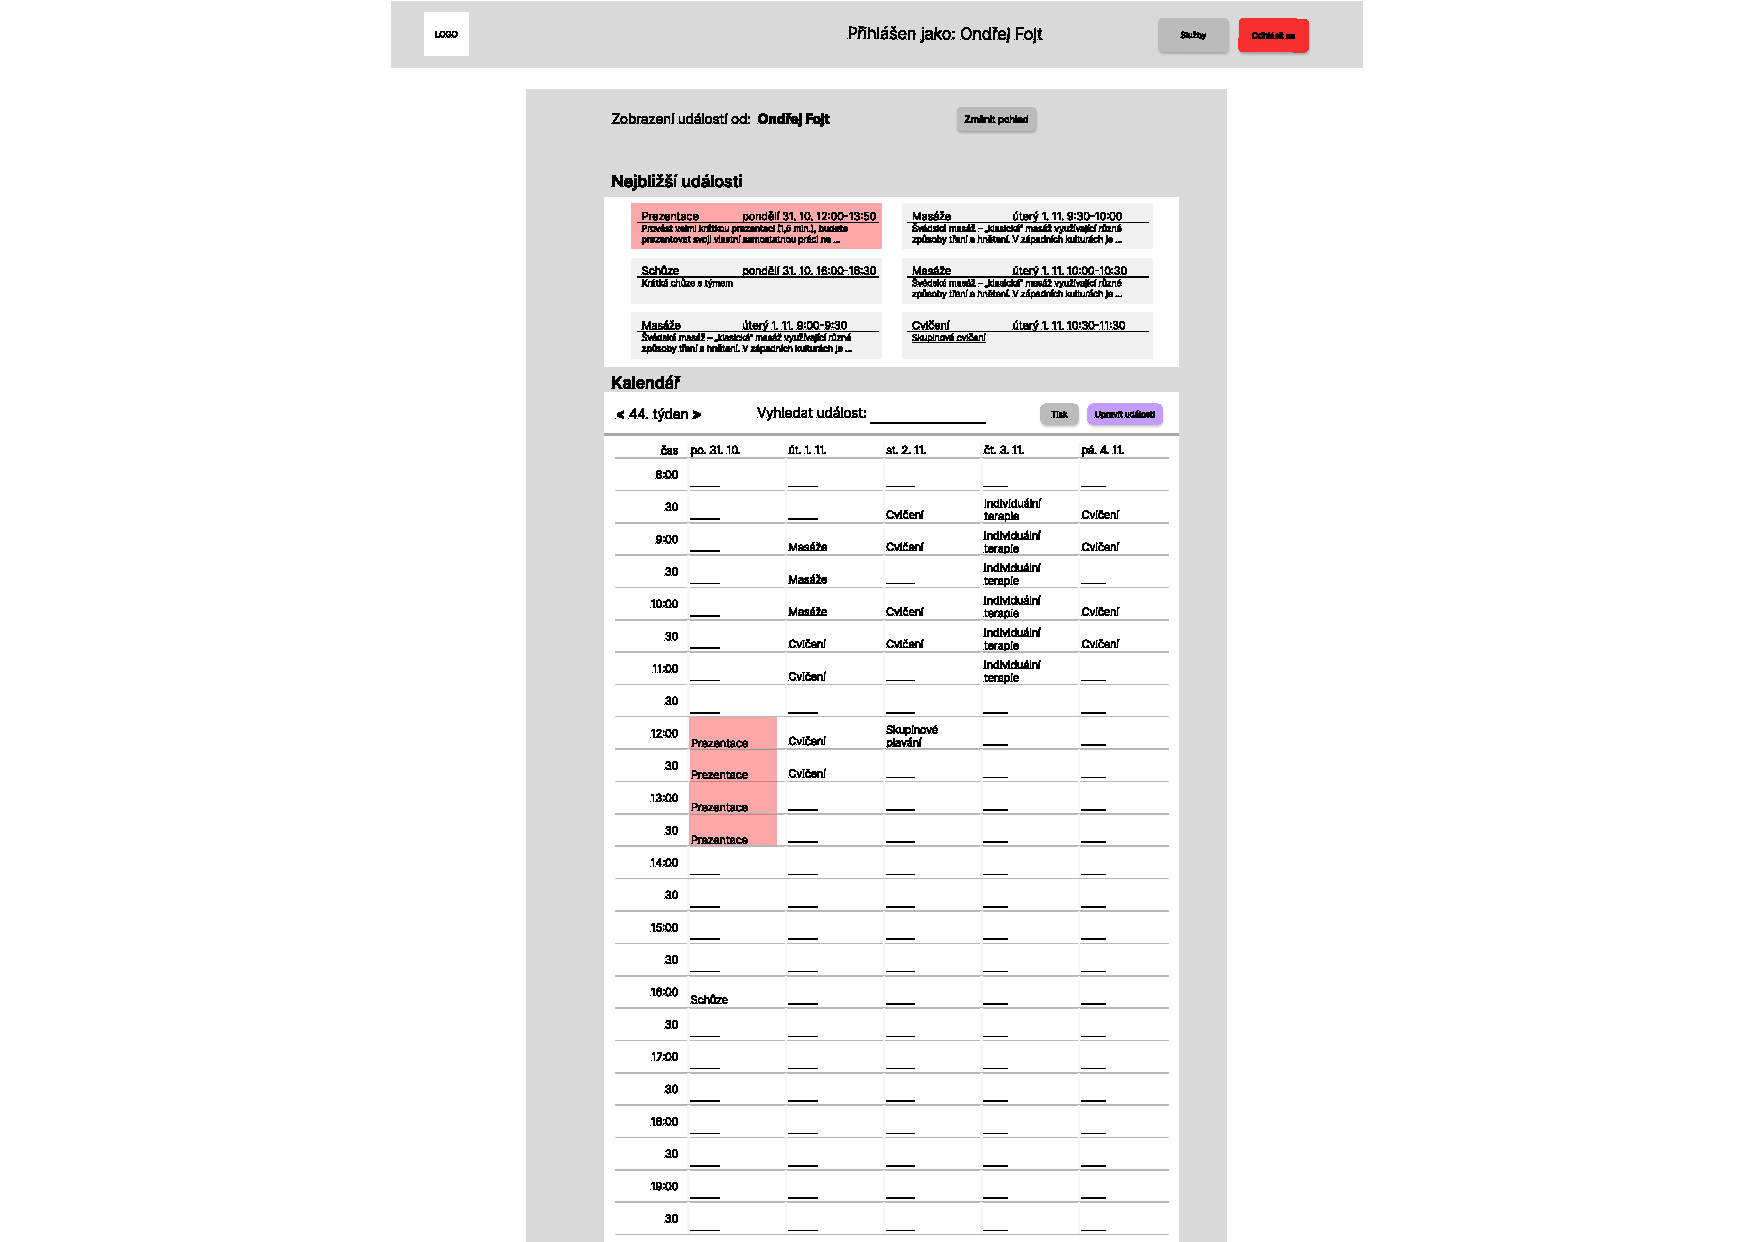
\includegraphics[width = \textwidth, trim=200 300 200 0, clip]{doc/latex/fig/ondra/figma1.pdf}
    \caption{Hlavní strana s výpisem nejbližších událostí a kalendářem událostí}
    \label{fig:Ondra_figma_mainpage}
\end{figure}

\begin{figure}[htbp]
    \centering
    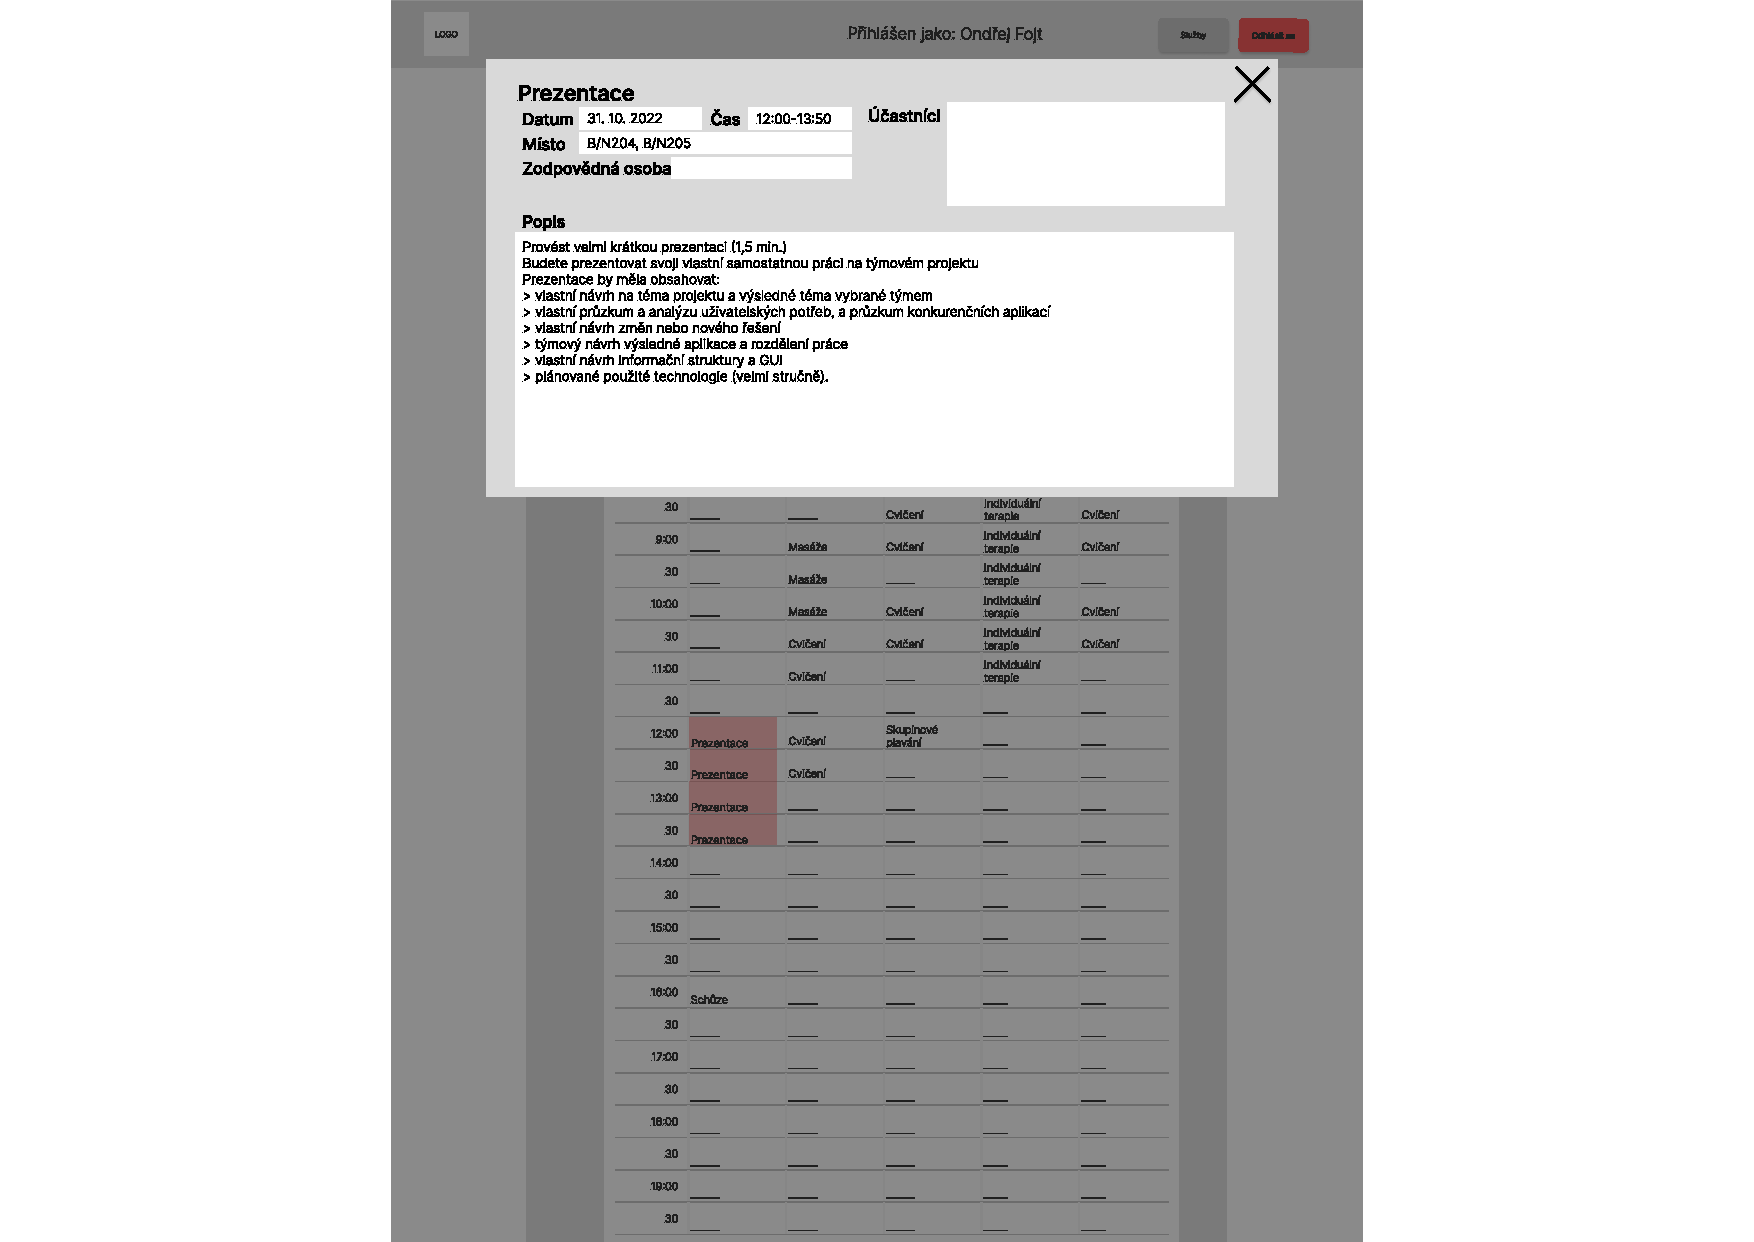
\includegraphics[width = \textwidth, trim=200 380 200 0, clip]{doc/latex/fig/ondra/figma2.pdf}
    \caption{Zobrazení údajů o události}
    \label{fig:Ondra_figma_event_detail}
\end{figure}

\begin{figure}[htbp]
    \centering
    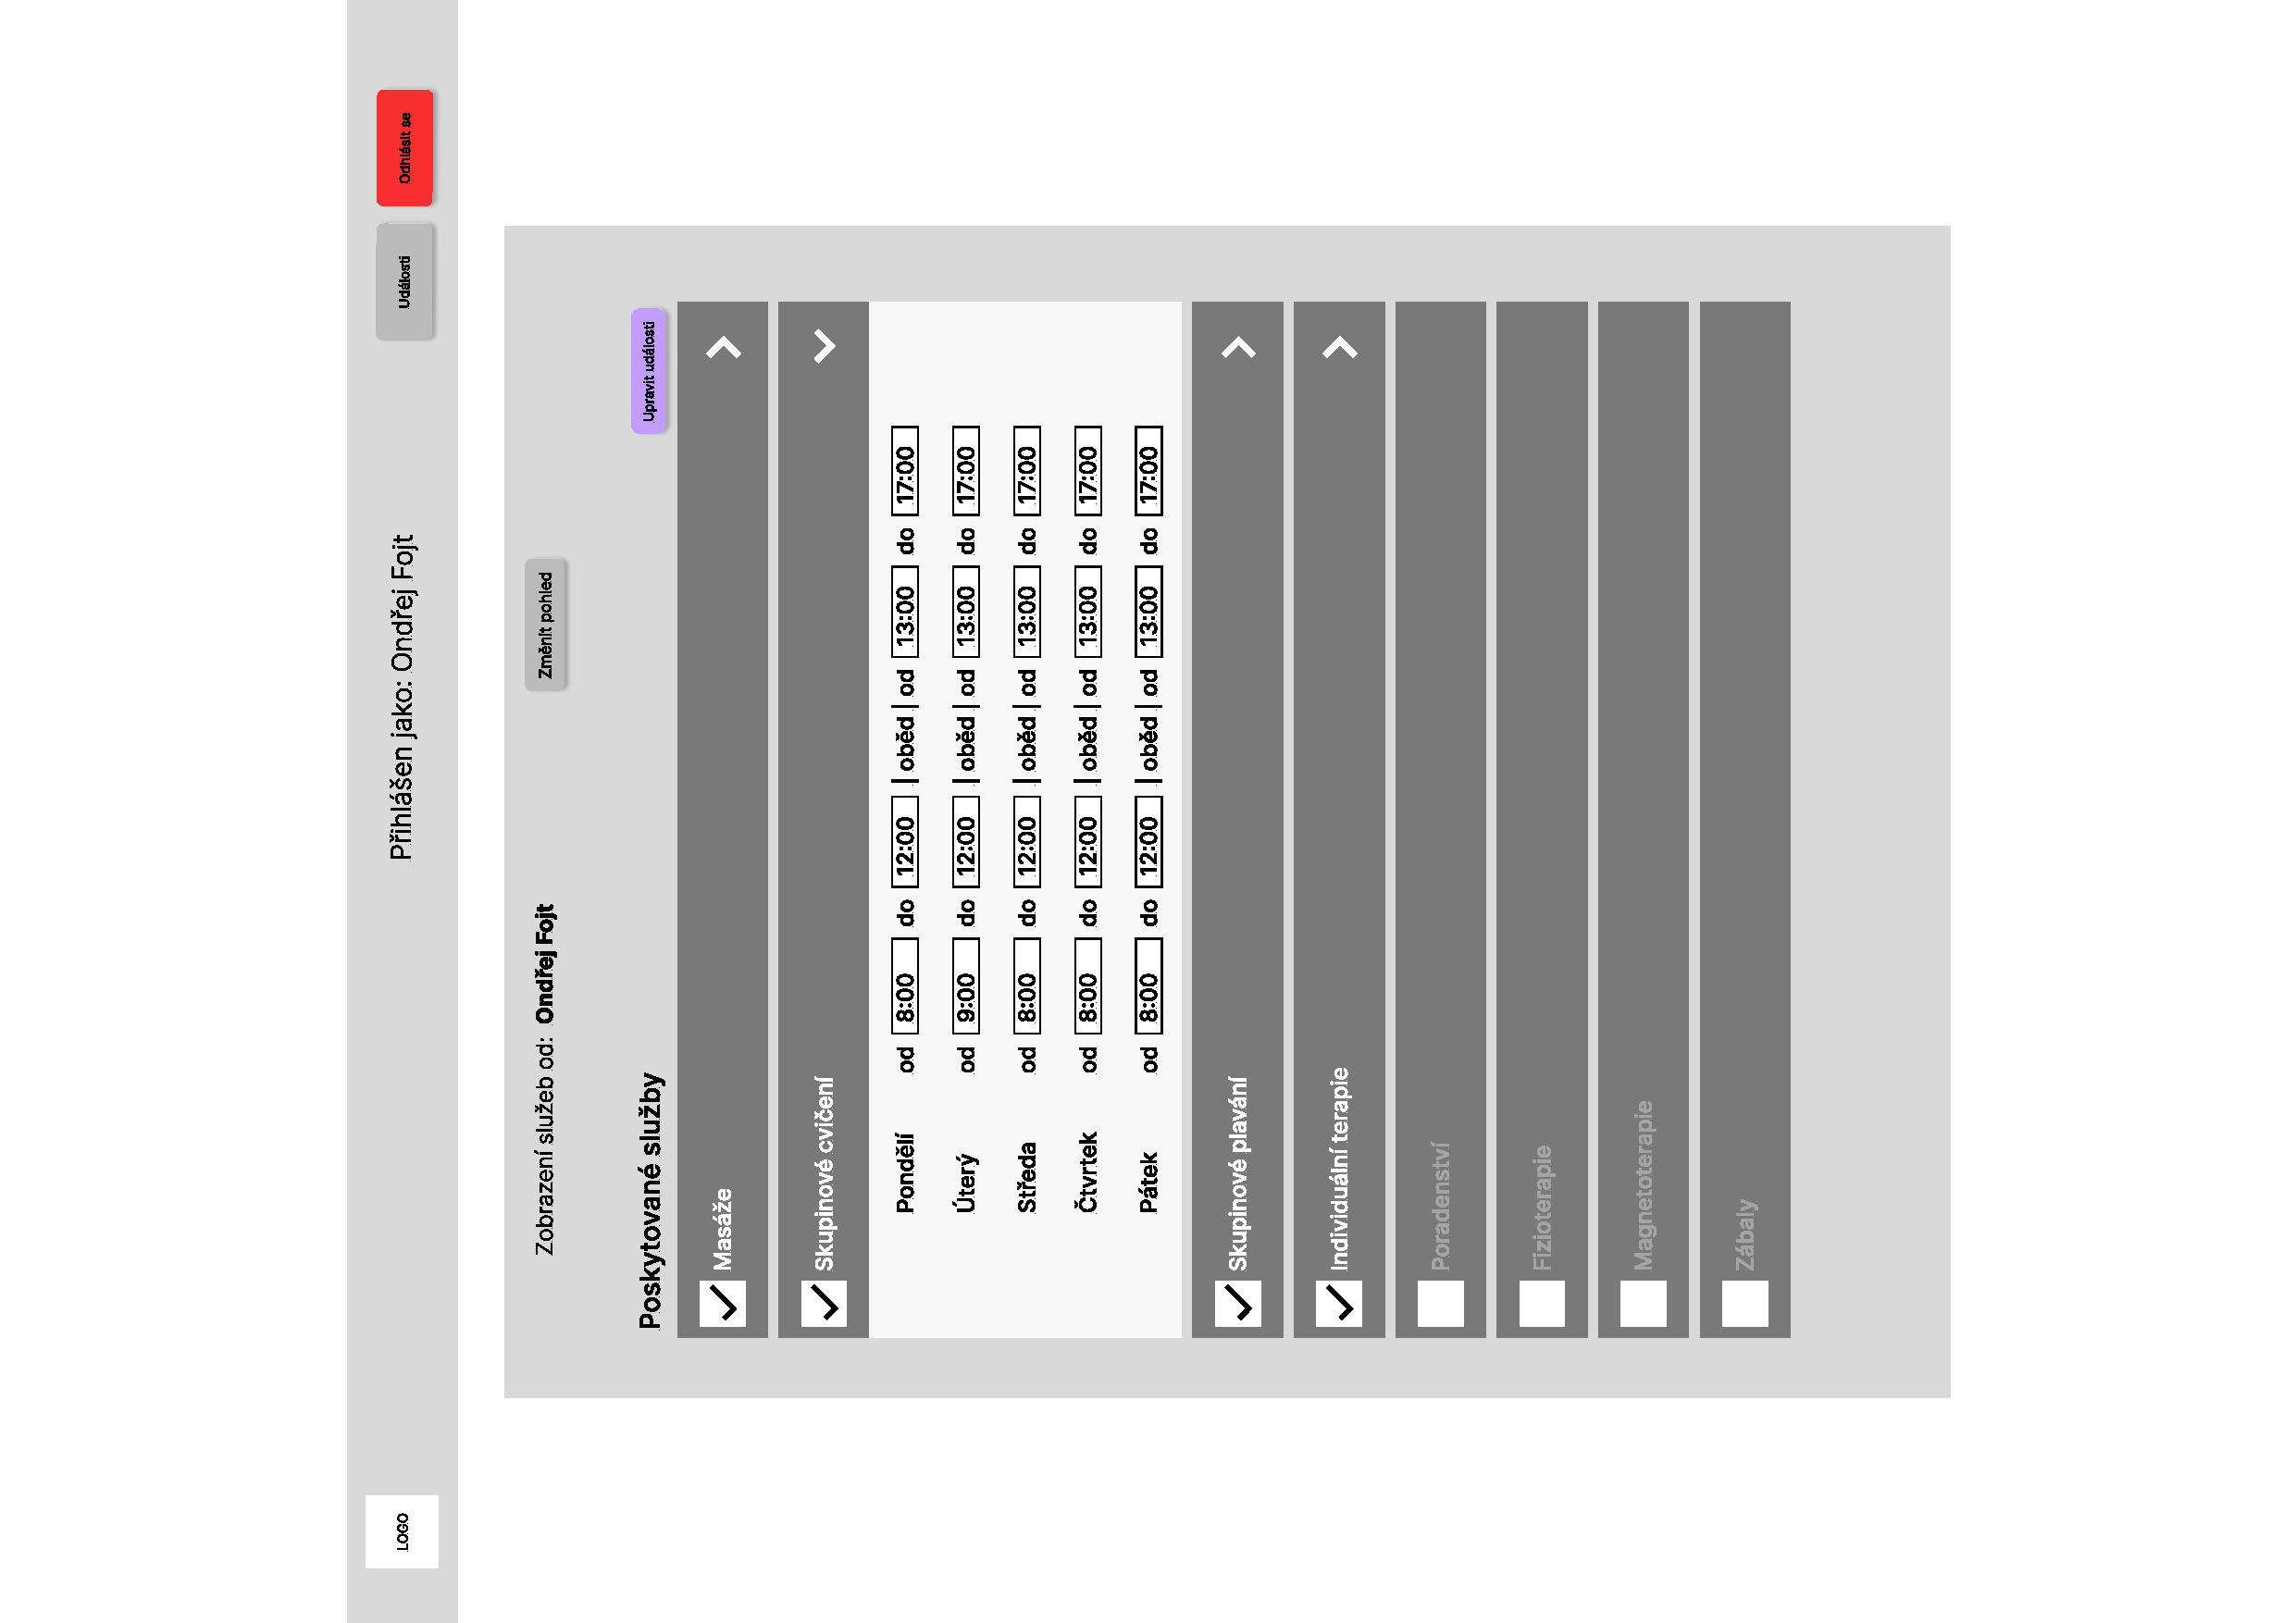
\includegraphics[angle=270, origin=c, width = \textwidth, trim=180 0 250 0, clip]{doc/latex/fig/ondra/figma3.pdf}
    \caption{Poskytované služby daného zaměstnance}
    \label{fig:Ondra_figma_services}
\end{figure}

\newpage

\subsubsection*{Testování makety}

Testována maketa pro zaměstnance výše a také pro přihlašování klientů od Vlada.
Testy byly provedeny na 3 osobách se zkušenosti z přihlašování na rehabilitace.
Testy spočívaly ve schopnosti orientace v systému a určování funkčnosti jednotlivých prvků.

Poznatky k přihlašování klientů:
\begin{itemize}
    \item Starší osoba může mít strach vkládat někde e-mail\\ pro přihlášení/registraci, kvůli reklamnímu spamu.
    \item Není jasný čas kdy se lze telefonicky spojit přímo se zaměstnancem, pokud by to bylo potřeba?\\ Někdy stačí přesměrovat hovor k vrátnici/sekretariátu.
    \item Některé osoby na rehabilitace přihlašuje například sestřička od doktora. Jak to máme z uživatelského hlediska vyřešené?
    \item Chybí cena za službu, popis dané služby a přehled přihlášky před potvrzením(ten je teoreticky odeslán v e-mailu, kde lze přihlášku zrušit... ale e-mail není 100\% spolehlivý)
\end{itemize}
Poznatky k rozhraní pro zaměstnance:
\begin{itemize}
    \item Každý se shodl, že nejbližší události by měli ukazovat pouze jeden den a že je potřeba zavést přepínání k tomuto poli mezi dny.
    \item Služby a organizační záležitosti firmy by potřeby barevné odlišení, které by nekolidovalo s odlišením nejbližší události.
    \item Nejde vyhledávat klienty.
    \item Pokud by se zobrazil kontakt na klienta tak by se hodilo vypsat, jejich termíny návštěv.
    \item Prvek \emph{Zobrazení událostí od} je buďto přehlížen nebo mu není věnována větší pozornost, především při prvním použití.
    \item Zajímavá otázka na back-end: Jakým způsobem se přidělí přihlášky zaměstnancům? Aby jeden neměl pořád přeplněno, protože má příjmení dříve v abecedě...
\end{itemize}

% README
% Pictures !!! include your own !!!
% When loading images, load zour images into fig. directory
% Then include them here and dont forget to fill capution and label please :)
%\begin{figure}[h]
%    \centering
%    \includegraphics[width = \textwidth]{doc/latex/fig/"your_image"}
%    \caption{"your_caption"}
%    \label{fig:"your_image_label"}
%\end{figure}

\subsection*{Provedené změny návrhu}

Zaměstnanec byl rozdělen na administrativního pracovníka, tedy zaměstnance, který vidí statistiky a obsazenosti služeb/procedur a zaměstnanců
a fyzioterapeuta, který je odpovědný za jednotlivé procedury.
Administrativní pracovník by měl mít také možnost přidávat a odebírat registrace pacientů na procedury.
Fyzioterapeut by měl moci potvrzovat příchod pacienta na registrace a vystavení zprávy o provedení zákroku.

Stránky pro tyto uživatele byly rozděleny členům týmu takto:
\begin{itemize}
    \item Ondřej Fojt - Administrativní pracovník
    \item Vít Hrbáček - Fyzioterapeut
\end{itemize}

\newpage

    \section{Samostatná práce člena týmu\ --\ Vít Hrbáček}
\label{sec:individual_work_vit}

\subsection{Výběr tématu, popis provedeného průzkumu s uživatelem, analýza uživatelských potřeb a klíčových problémů, navržená sada změn}

\subsubsection*{Výběr tématu}

{\large Můj hlavní návrh:}

Plugin pro vložení fóra do předešlého školského informačního systému VUT FIT


{\noindent \large Vedlejší návrh:}

Informační systém pro správu promítání kina a zakoupení vstupenek uživatelem

\subsubsection*{Provedený průzkum}

{ \noindent \large Rezervační systém pana doktora Bidla pro domluvení konzultací:}

Domluvil jsem si osobní konzultace s doktorem Bidlem ohledně probrání jeho uživatelského pohledu rezervačního systému, takže jsem měl to štěstí zrovna vyzkoušet jeho systém v praxi. Doktor Bidlo mi na konzultacích vyprávěl, že v minulosti domlouval konzultace přes emaily. Fungovalo to tak, že vypsal všechny termíny, kdy je k dispozici a student také. Bylo občas složité se přes maily domluvit. Vytvořil si proto na míru aplikaci, která mu s tím pomohla. 
\noindent\emph{ \ref{fig:Vit_n}.}

\begin{figure}[htbp]
    \centering
    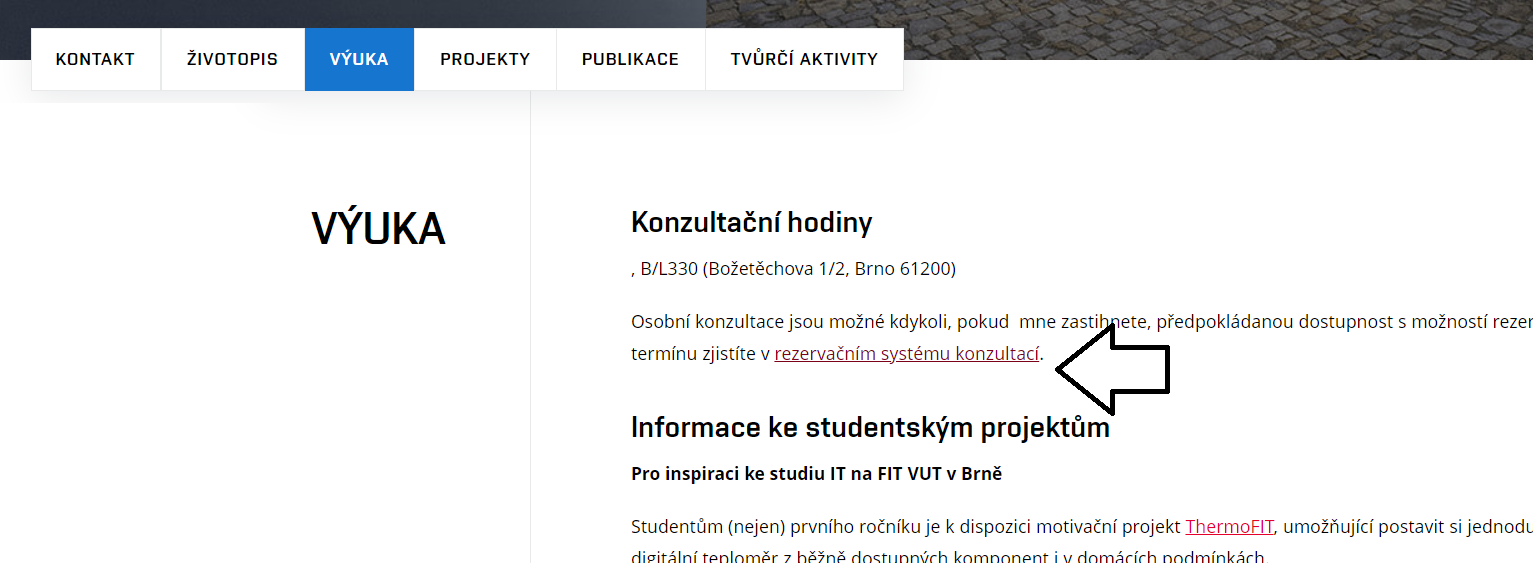
\includegraphics[width = \textwidth]{doc/latex/fig/vit/1.png}
    \caption{Defaultní stránka pro hledání informací o konzultacích zaměstnance fakulty}
    \label{fig:Vit_n}
\end{figure}


\subsubsection*{Analýza potřeb a klíčových problémů}

Program slouží všem uživatelům k tomu, aby studentům zprostředkovával informace o dostupnosti termínů na doktorovy konzultace. Na veřejných stránkách vedle výpisu termínu konzultací má odkaz na stránku s rezervacemi konzultací.

\subsubsection*{Navržené změny}
Pan doktor byl velice šikovný. Jako bývalý student znal potřeby svých studentů a sám sebe, tak si systém vytvořil, jak by měl vypadat podle svých vlastních představ. Díky tomu není moc vylepšení uživatelského rozhraní. Jediné, na co jsme přišli bylo, že pro uživatele je neintuitivní napsat svůj login (identifikátor studenta na fakultě doktora Bidla) do políčka představující volný termín. Jako vhodné vylepšení lze navrhnout změnit políčko na tlačítko po kterém se zobrazí vyskakovací okno, kde by uživatel vypsal svůj login. Doktor Bidlo vybral login jako jedinou potřebnou informaci, kterou musí student zapsat kvůli tomu, že student nemusí zadat mnoho a doktor Bidlo jednoduše z něho zjistí studentovo jméno a e-mailovou adresu.

\newpage
\subsection{Popis současného řešení\ --\ jaké nástroje uživatel používá, \\
popř. obrázky/screenshoty současného řešení/reálné situace}

\noindent\emph{Výměna rozvrhů} 
\begin{itemize}
    \item[+] Dostačující v případě mírného zájmu o konzultace
    \item[--] Časově náročné
    \item[--] Administračně náročnější
	\item[>] Někteří vyučující mají pevně vypsané konzultační hodiny. Řeší to snazší organizaci, ale v praxi nikdo nemusí přijít.
\end{itemize}

Rezervační systém doktora Bidla je mnohem efektivnější. Stránka obsahuje rozvrhy pana Bidla v několika následujících týdnech. Volné termíny, kdy je možné ho fyzicky potkat na škole jsou zeleně a termíny, kdy je dostupný online, jsou žluté. Student si může vybrat jakýkoliv dostupný termín. 

\begin{figure}[htbp]
    \centering
    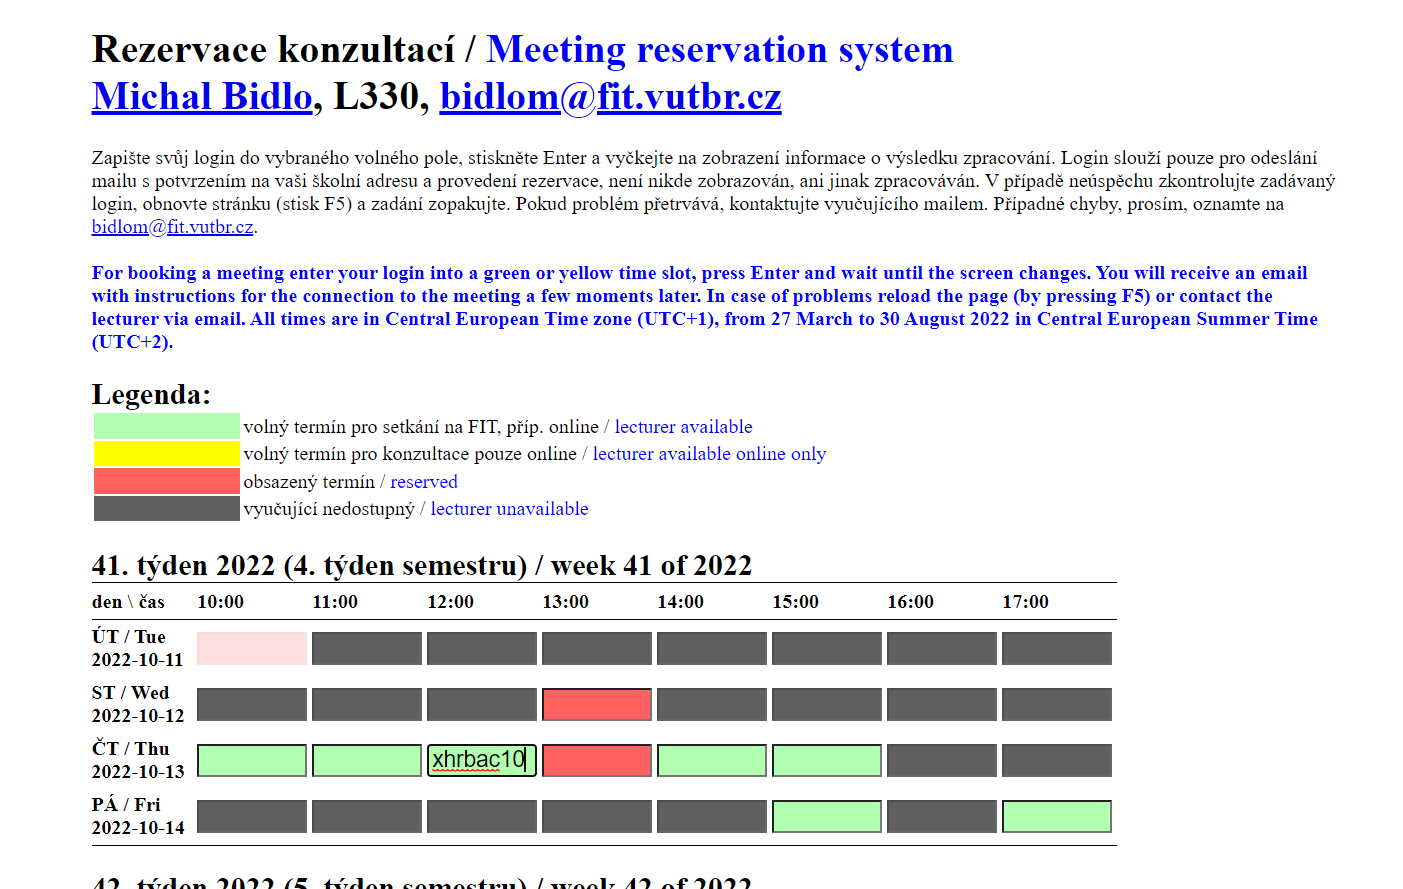
\includegraphics[width = \textwidth]{doc/latex/fig/vit/2.png}
    \caption{Snímek obrazovky Bidlova rezervačního systému}
    \label{fig:Vit_k}
\end{figure}

Termín se rezervuje zapsáním školního loginu do volného pole\\ a~zmáčknutím enter.
Výhodou je nutnost odeslat minimum dat a netřeba se registrovat a přihlašovat na stránku. Nevýhodou je již zmíněné neintuitivní pochopení systému. Je potřeba si přečíst nápovědu výše pro pochopí, co se od uživatele očekává. Zapsaní studenti jsou schválně na stránce anonymní. Po odentrování se zobrazí hláška o úspěchu či neúspěchu rezervace. Líbí se mi, že je zde i odkaz na mapu s umístěním místnosti, kde se konzultace konají. Je to totiž přesně informace, kterou by student o doktorovi jinak musel vyhledávat. Zároveň systém pošle dva emaily. První je potvrzení na studentův email, který zjistil podle jeho školního loginu, a upozornění o nové konzultaci na email pana doktora. Panu doktorovi vyhovuje, že nemusí procházet denně další stránku, ale pípne mu na telefonu, že mu někdo přijde na konzultace. Hodí se to i na konzultacích na poslední chvíli. Uživatel může zadat konzultaci na brzký termín a doktor se o ní snadno doví. 
Termín si může student zrušit pomocí odkazu v emailu. Aplikace, mimo emailu zaslanému panu doktorovi, nemá žádné jiné uživatelské rozhraní. Pan doktor může v případě potřeby přímo studentský login vepsat. Pan doktor používá systém tak, že mu přijde notifikace na nový email. Studenti zmíněným způsobem. Z pohledu studenta, který si konzultace rezervoval mi program vyhovoval. V době koronavirusu zaslal software s mírnými úpravami i jiným přednášejícím, ale nikdo neprojevil zájem.

\subsection{Návrh uživatelského rozhraní, makety rozhraní, testování pomocí maket rozhraní}

\emph{Část projektu v týmu: Návrh rozhraní pro nepřihlášeného uživatele}

\subsubsection*{Návrh}

\begin{itemize}
    \item Lze snadno najít volné termíny
    \item Uživateli je poskytnuta možnost rezervace zvoleného termínu
    \item Jednoduché zobrazení podrobností o události
    \item Do emailu by mu přišlo potvrzení o zarezervování a možnost zrušení rezervace
\end{itemize}

\subsubsection*{Maketa}

{\noindent\large Popis makety}\\
Uživateli je nabídnuto čisté přehledné prostředí s rozvrhem znázorňující volná a obsazená místa. Pro snadné a intuitivní pochopení uživatele jsou dostupné termíny vždy zelené. Zaregistrované termíny jsou již červenou barvou. V případě nemoci, dovolené či podobně může být termín nedostupný, ale nezarezervovaný. V tomto případě jsou termíny označeny šedou barvou značící neaktivní termín. 

Pro snadný přehled má vypsáno v jakém týdnu se jeho náhled nachází. Svůj náhled může změnit pomocí přechodu doprava (následující týden) či zpět doleva. 

Na moji maketu se lze podívat \href{https://www.figma.com/file/4nOyfGc52uArBuMkx1NhXb/Untitled}{na odkazu zde.}

\begin{figure}[htbp]
    \centering
    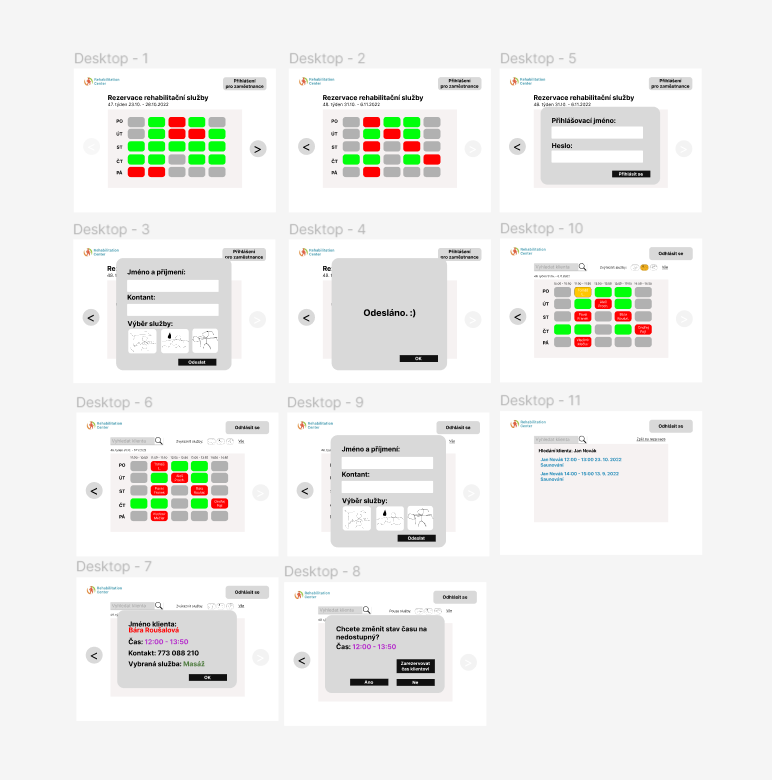
\includegraphics[width = \textwidth]{doc/latex/fig/vit/3.png}
    \caption{Obrázek vytvořeného návrhu rezervačního systému pro Wellness centrum}
    \label{fig:Vit_k2}
\end{figure}

\newpage
\subsubsection*{Testování makety}
Maketa byla aktivně testována na třech uživatelích.\\
Starší uživatel měl problémy se správným pochopení tlačítek, které obsahují text a jeho práce byla pomalejší. Mladší uživatelé zvládli všechny úkoly udělat rychle a snadno se v rezervačním systému orientovali, ač tam byly úplně poprvé. Mladší uživatelé se neptali vůbec. Starší uživatel se často ujišťoval, zda provádí akci správně. Testování makety naštěstí proběhlo úspěšně. 


\newpage


    \section{Společně odvedená práce}

\label{sec:team_work}

\subsection{Důvod vybrání tématu týmem}
Téma Rezervačního systému se nám líbilo nejvíce. Zaujala nás rada od zkušeného programátora, který podotkl, že rezervačních systému je na trhu nedostatek. Je jistě užitečnější vytvořit program, který se někomu možná bude jednou hodit.

\subsection{Analýza uživatele - co uživatel dělá v reálném životě, jaký je\\
proces/činnost, kterou vykonává a kde by mu příp. vhodný SW mohl
pomoci}
Každý člen našeho týmu si zvolil uživatele s jiným zaměřením.
Námi vybraná skupina uživatelů jsou poskytovatelé služeb. Každý z nich má v nabídce paletu služeb, které poskytuje svým zákazníkům.
Problém ale nastával při domlouvání realizace samotné služby. Nejčastěji se jednalo o chybu "v lidském faktoru". Na recepci seděl člověk a ten rezervace spisoval.
Rezervace byly špatně poznačené nebo poskytovatelé zapomněli informovat zákazníky o zrušení apod.
V případě online rezervačního systému by byla rezervace ponechána klientovi, čímž by se mohlo předejít už nahoře zmíněným chybám lidského faktoru.
Systém by rovněž informoval zákazníka obratem o stavu rezervace a uměl by taky informovat o nastávající rezervaci apod.


\subsection{Potřeby uživatele - co je cílem činnosti, čeho chce dosáhnout}
V případe poskytovatele služeb, každý z nich potřeboval:
\begin{itemize}
    \item možnost vytvoření rezervace pro jimi nabízené služby
    \item minimalizovat potřebu interakce s klienty - časově náročné
    \item potvrzení a informování zákazníků o vytvořené rezervaci
    \item editace rezervace
    \item jednoduchost systému
\end{itemize}

\subsection{Shrnutí současných řešení a výsledné pro a proti, inspirace, nápady}
V současné době se na trhu vyskytuje nedostatek služeb, které nabízí nějakou formu rezervačního systému. Rezervační systém typu
"papír a pero" nám sloužil jako šablona dat, která byla zapotřebí při vytváření systému.
Webové aplikace, které již na trhu existují jsou sice jednoduché na používání, ale pro klienty. Pro poskytovatele služeb se jednalo častokrát
o neefektivní a drahé řešení ve formě SW "šitého na míru" či webová aplikace, která má až zbytečně moc nepotřebné funkcionality. T.j
poskytovatel služeb zbytečně platil za něco, co nevyužívá.


\subsection{Návrh zadání - co má nové řešení zlepšit, co uživateli umožní, v čem
mu konkrétně pomůže, co uživateli konkrétně přinese, co má být
konkrétním výstupem, jak má vypadat nový uživatelský proces}

Při vytváření makety jsme se inspirovali již existujícími aplikacemi zmíněných v individuálních řešeních u jednotlivých členů týmu.
Při ladění jsme se drželi programátorských taktik KISS. Snažili jsme se dát uživatelům, co nejméně možností ztratit se v rozhraní.
T.j. naše řešení obsahuje co nejméně prvků, se kterými mohou interagovat.
Stačila nám základní funkcionalita, tedy vytváření a editace rezervací.
Zároveň jsme přihlédli na způsob, jak připojit aplikaci k již existující stránce poskytovatele. Věříme totiž, že internetová
stránka je v 21. století nutností a tím pádem jsme se rozhodli pro jednoduché připojení stránky s aplikací ve formě pluginu.
Tedy na stránce bude odkaz na samotnou aplikaci ve formě tlačítka nebo jiného hypertextového odkazu, která bude běžet na stejném
serveru, jako stránka poskytovatele. Jednalo by se tedy o nejminimalističtější řešení pro webovou aplikaci a tím pádem by bylo ve
výsledku potřebné minimum pro samotnou rezervační aplikaci

\newpage
\begin{figure}[h]
    \centering
    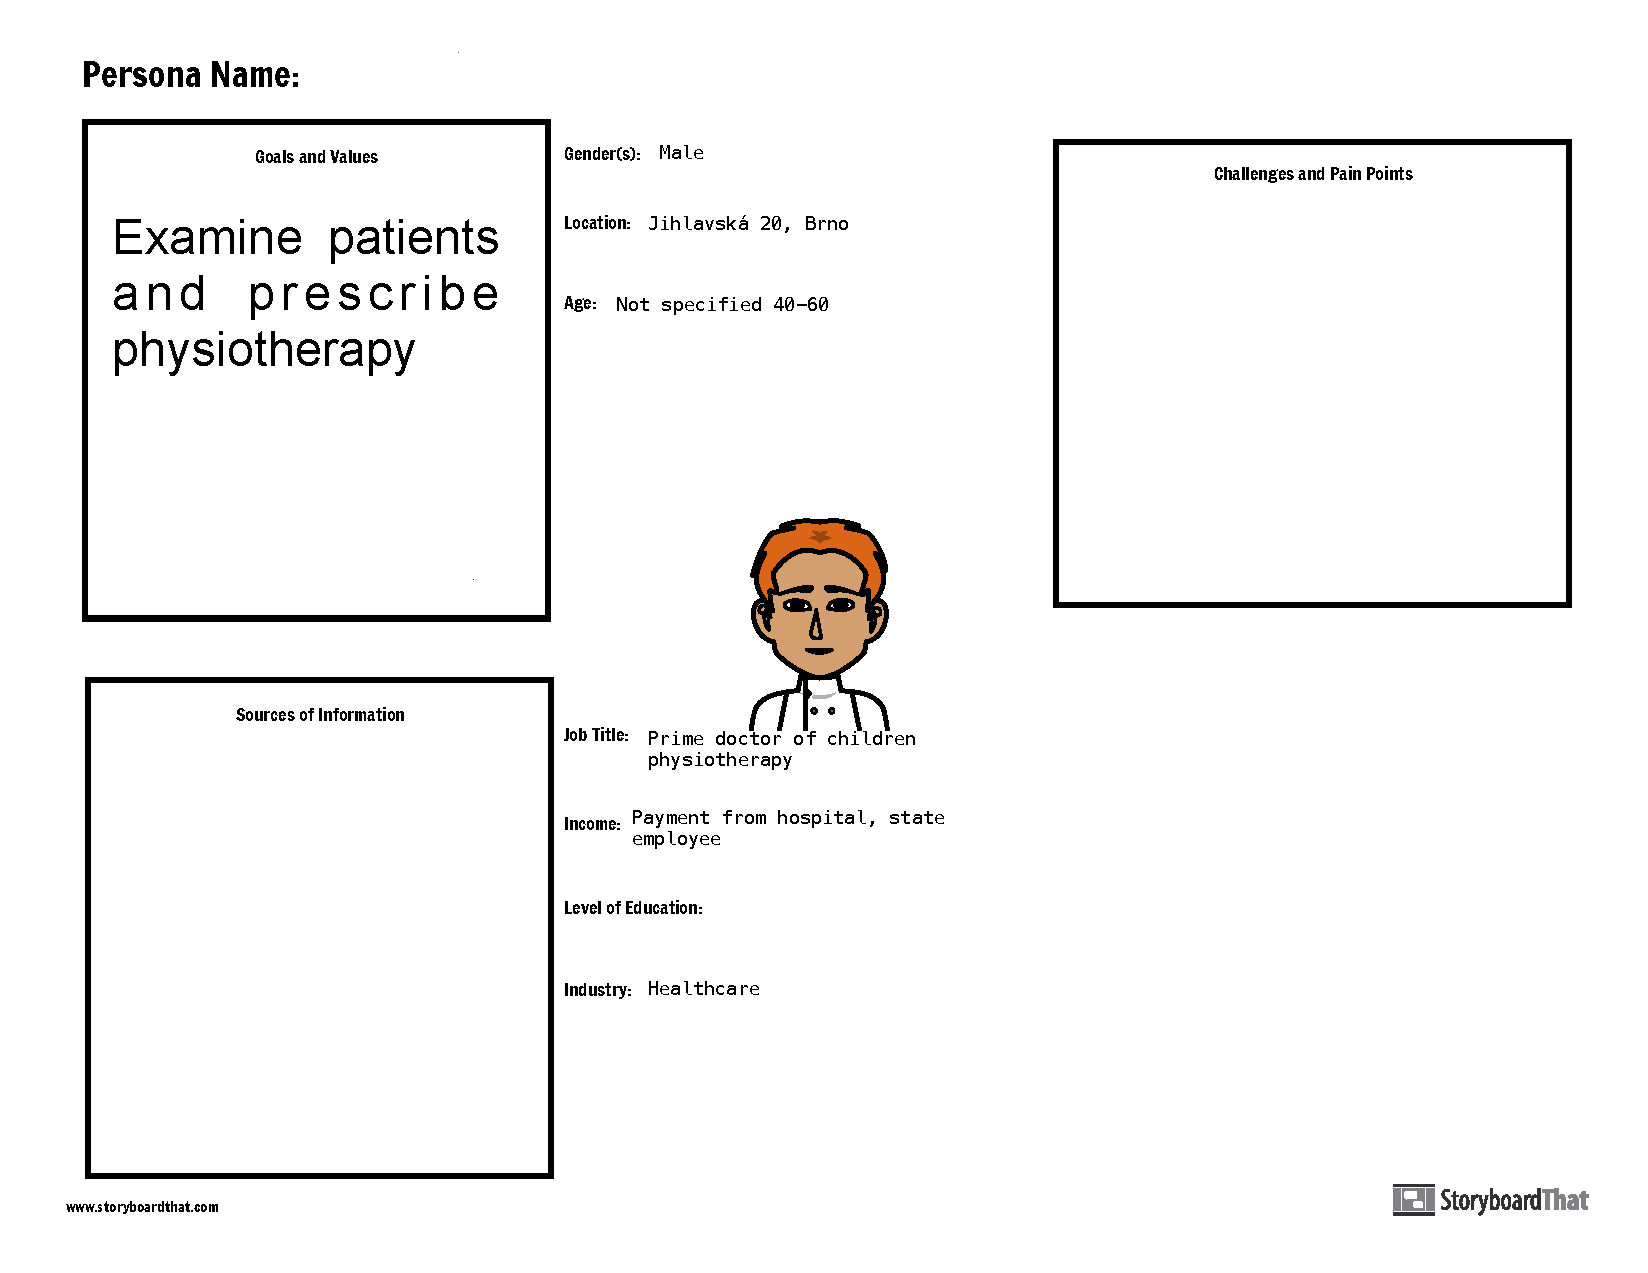
\includegraphics[width=1.4\textwidth, angle=270]{doc/latex/fig/vlado/Persona_Worksheets_PDF_dragged.pdf}
    \caption{Doktor}
    \label{fig:pers_doctor}
\end{figure}

\begin{figure}[h]
    \centering
    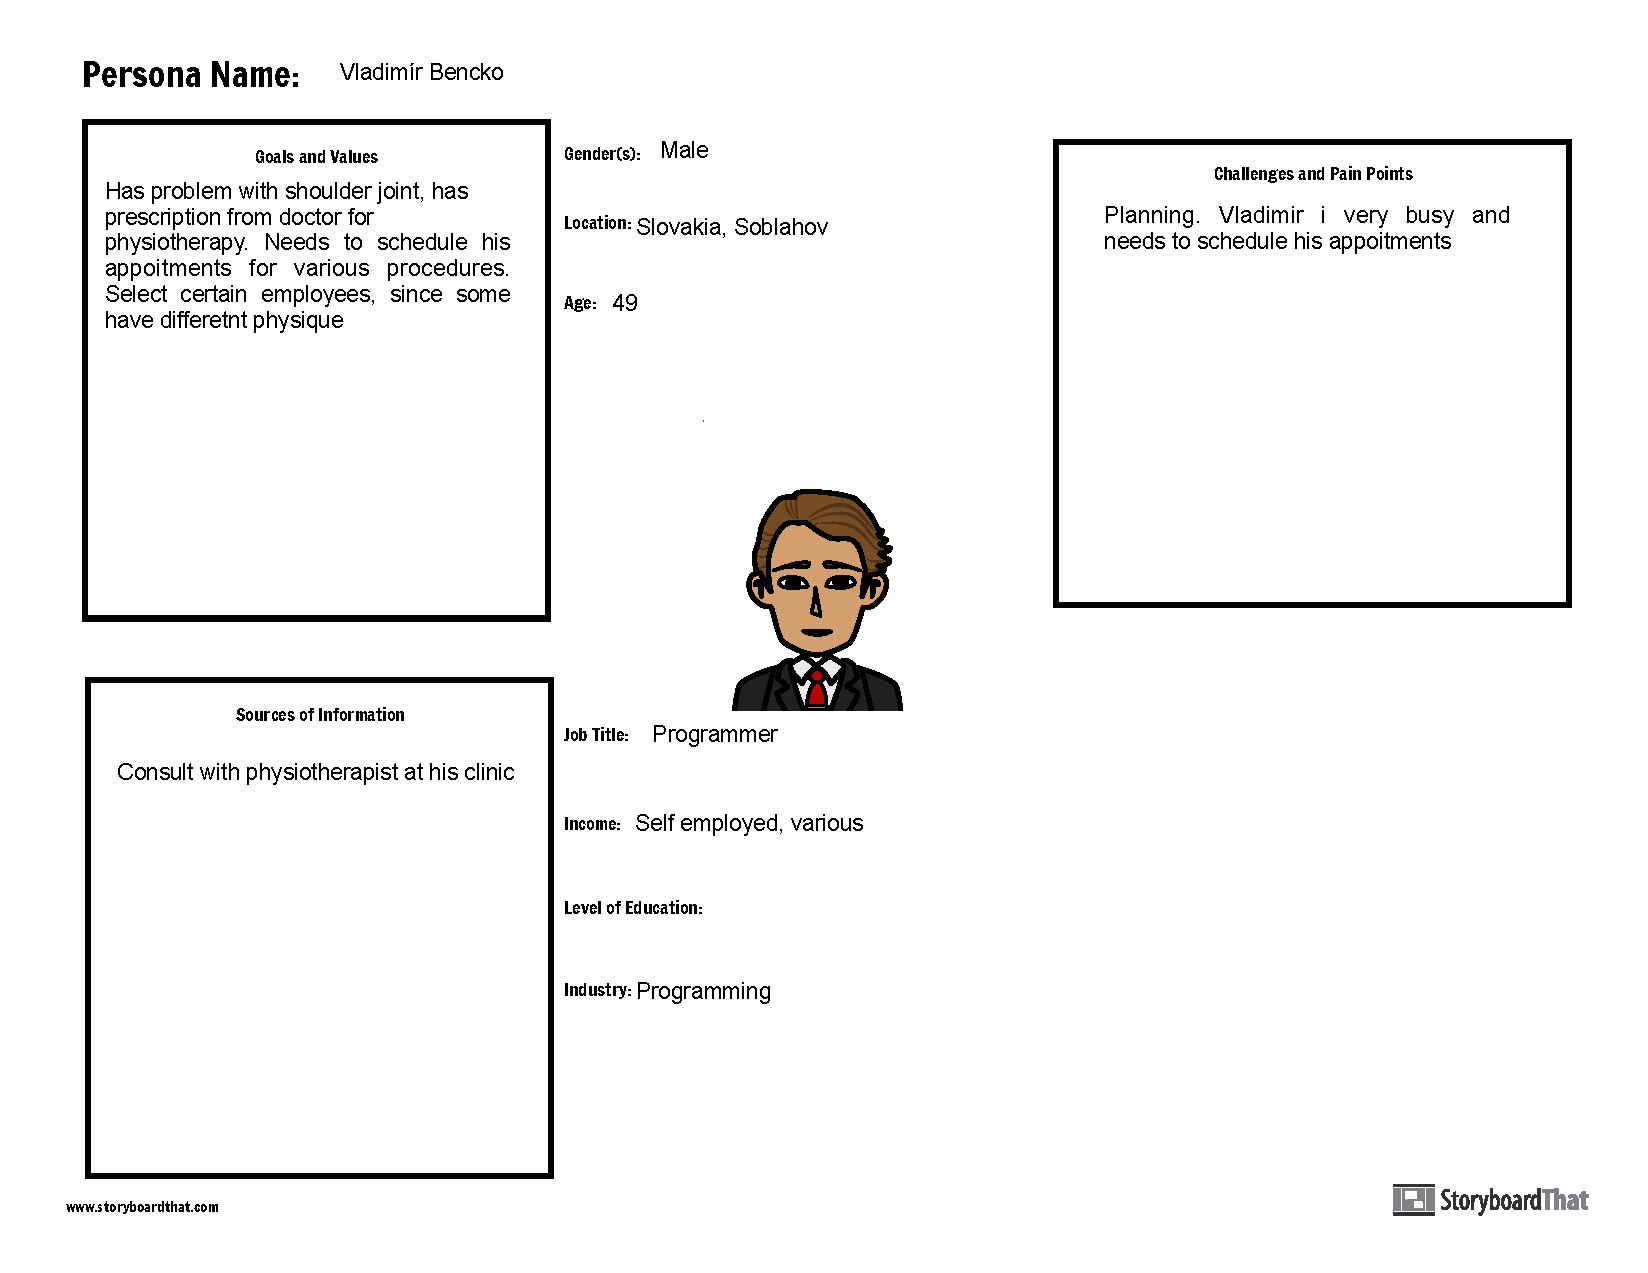
\includegraphics[width=1.4\textwidth, angle=270]{doc/latex/fig/vlado/Persona_Worksheets_PDF_dragged_2.pdf}
    \caption{Pacient}
    \label{fig:pers_patient}
\end{figure}

\begin{figure}[h]
    \centering
    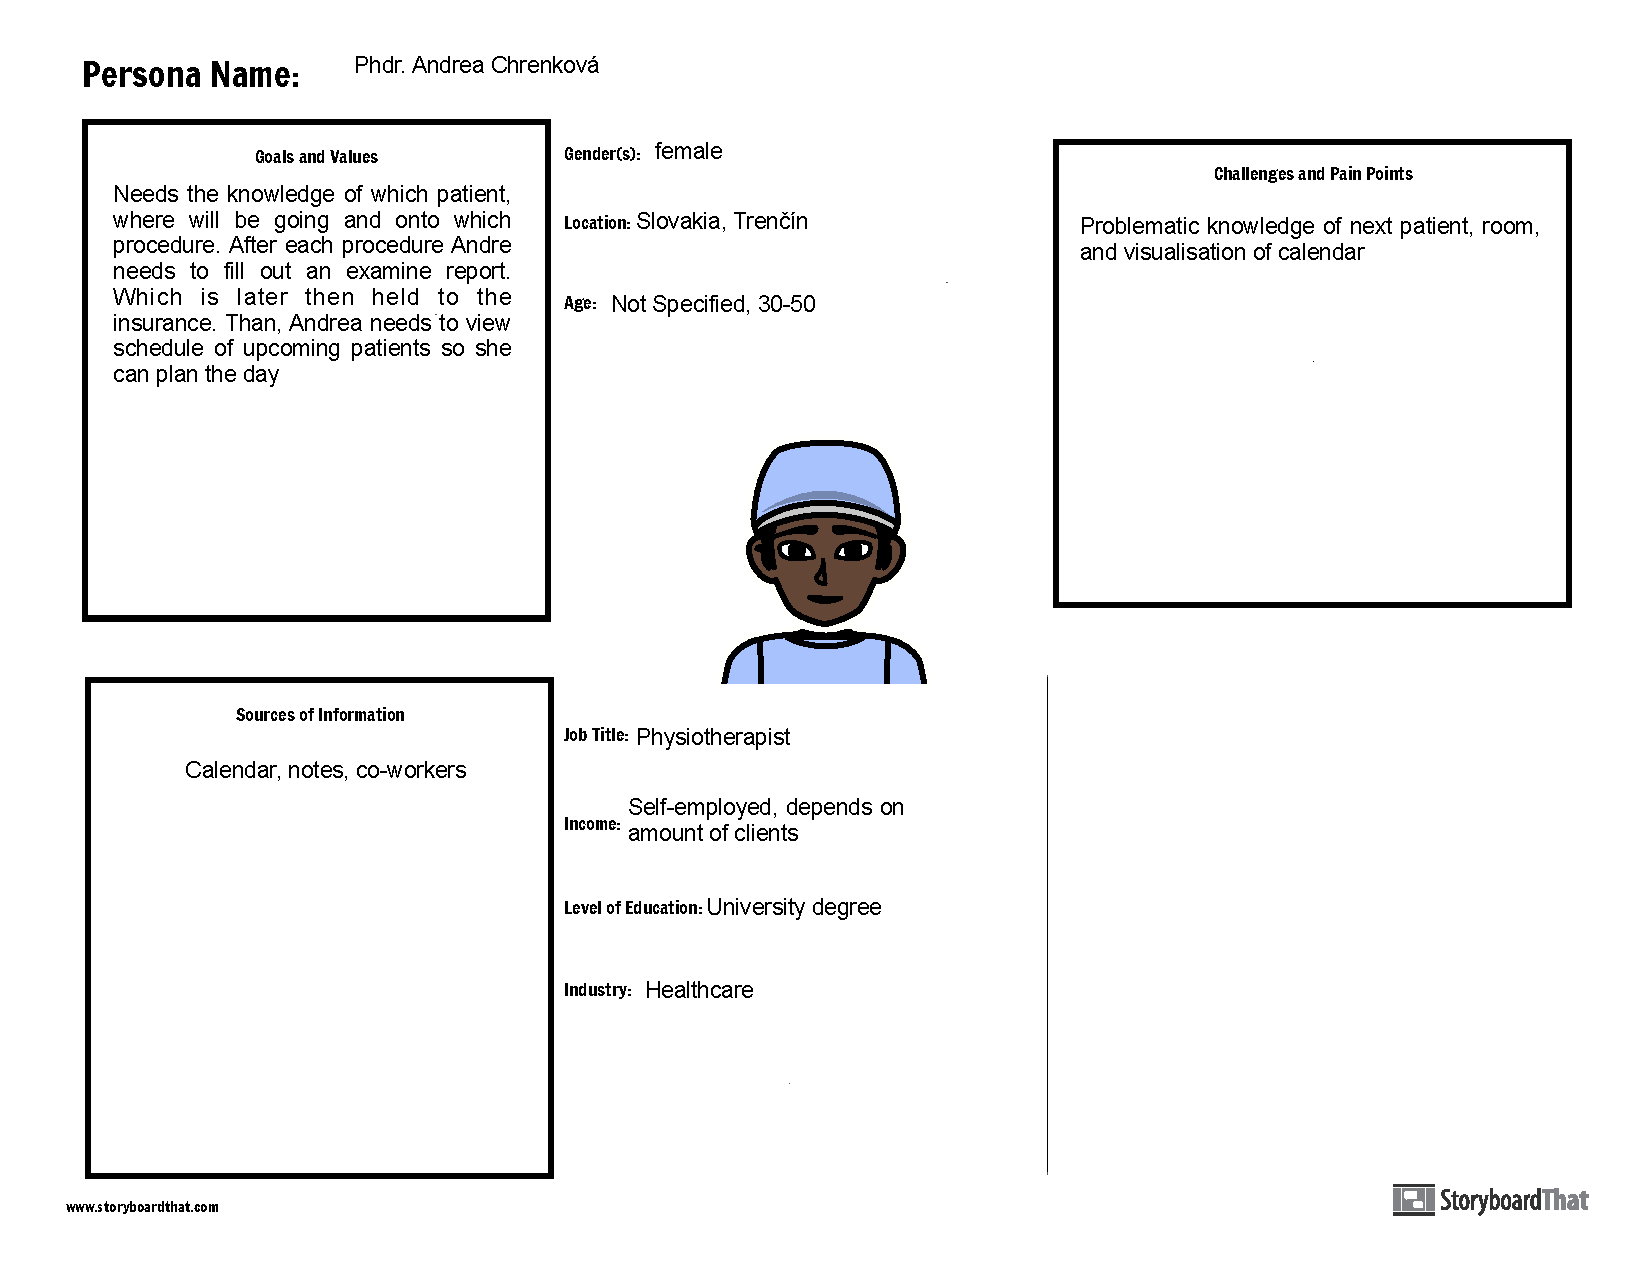
\includegraphics[width=1.4\textwidth, angle=270]{doc/latex/fig/vlado/Persona_Worksheets_PDF_dragged_3.pdf}
    \caption{Fyzioterapeut}
    \label{fig:pers_physio}
\end{figure}
\newpage



\subsection{Návrh řešení (předběžný) - nákresy vlastního řešení, datový model
    (datové struktury), popis API.}
Máme několik nápadu na popis API. Zatím jediný realizovaný způsob byl založen na komunikaci se serverem, který ukládá rezervace a posílá seznamy rezervací.
Zatím jsme kód nechali běžet\\ na bezplatném webhostingu Webzdarma.cz. Rezervace se dá na server poslat například pomocí \begin{quote}
    \href{https://iturezervacnisystem.wz.cz/index.php?jmeno=Vit}{https://iturezervacnisystem.wz.cz/index.php?jmeno=Vit}
\end{quote}. Server přijme atributy nazvané jmeno (viz. ukázka), den, mesic, rok, od, do, prijmeni, email, telefon, komentar, kategorie (kategorie služby jako masáže, sauny apod.) a specifikace (např. masáž obličeje). Pomocí příkazu nejblizsi=true lze zjistit nejbližší termíny. Příkaz rezervaceDanehoDne=true vypíše rezervace podle zvolených atributů den, měsíc a rok. Data vypisuje v formátu JSON. Technologii XML jsme použili pro načítání seznamu aktuálně nabízených služeb. Finální backend a API nakonec se vylepšila a začala nabízet více služeb pro práci s daty.

\newpage

\subsection{Testovnie aplikacie} \label{client_testing}

\subsubsection{Testovanie rozhrania pre klienta}
Testování proběhlo na dvou kamarádech z internátu, oba dva s problémy s páteří. \\
Testované prěbehlo vyzkoušením rozhraní.\\
Kvalita programu byla oproti referencnímu řesení snížena, avšak testovacím subjektům sa nelíbila minimalitičnost stránky.
Funkcionalita oproti referenčnímu řešení byla včak zachována.


Testovaná osoba 1

Záznam:
\textit{"Jednoduché, možno až moc. Pekne potriedené, mohlo by byť viac farebné. Zvolil som si masáž, prečo nie, po kliknutí sa
mi zobrazia viaceré možnosti,
dobrý nápad. Výber zamestnanca ... Výber dátumu. Prehľad dátumov je pekne spravený, zoradenie pod seba mi vizuálne
dobre oddeluje dátumy. Vyplnenie
osobných údajov ... mǒže byť. Aj komentár po vyplnení, fajn."}

Závěr:
\textit{"Viem o čo ste sa pokúšali, vyzerá to byť veľmi jednoduché. Mohlo by byť viac farebné. Ale objednať cez to sa dá.
Nie je to hrozné, nie je to výborné. Stačí to."}


Testovaná osoba 2

Záznam:
\textit{"Stránka na prvý pohľad mi príde minimalistická, základ. Farebná schéma nie je pekná ale postačujúca. Vyberte si službu
... biolampa. Vyberte si zaměstnance ...
tak isto ako predtým, proste obyčajné, biele, jednoduché ale prehľadné, nestratím sa v tom. Vyberte si datum, a tak,
dajme tomu utorok o deviatej ráno.
Tak isto ako predtým, úplne jednoduché.
Vyplnte své údaje, napíšem nejaké testovacie údaje. Odoslať."}

Závěr:
\textit{"Celkom v pohode. Jediné čo by osm dodal je, že mi to príde veľmi jednoduché, stránka je nezáživná a všetko je príliš
minimalistické."}

\newpage

\section{Sreenshoty z aplikacie}

\subsubsection{Rozhraní pro klienta}

\begin{figure}[h]
    \begin{subfigure}{.5\textwidth}
        \centering
        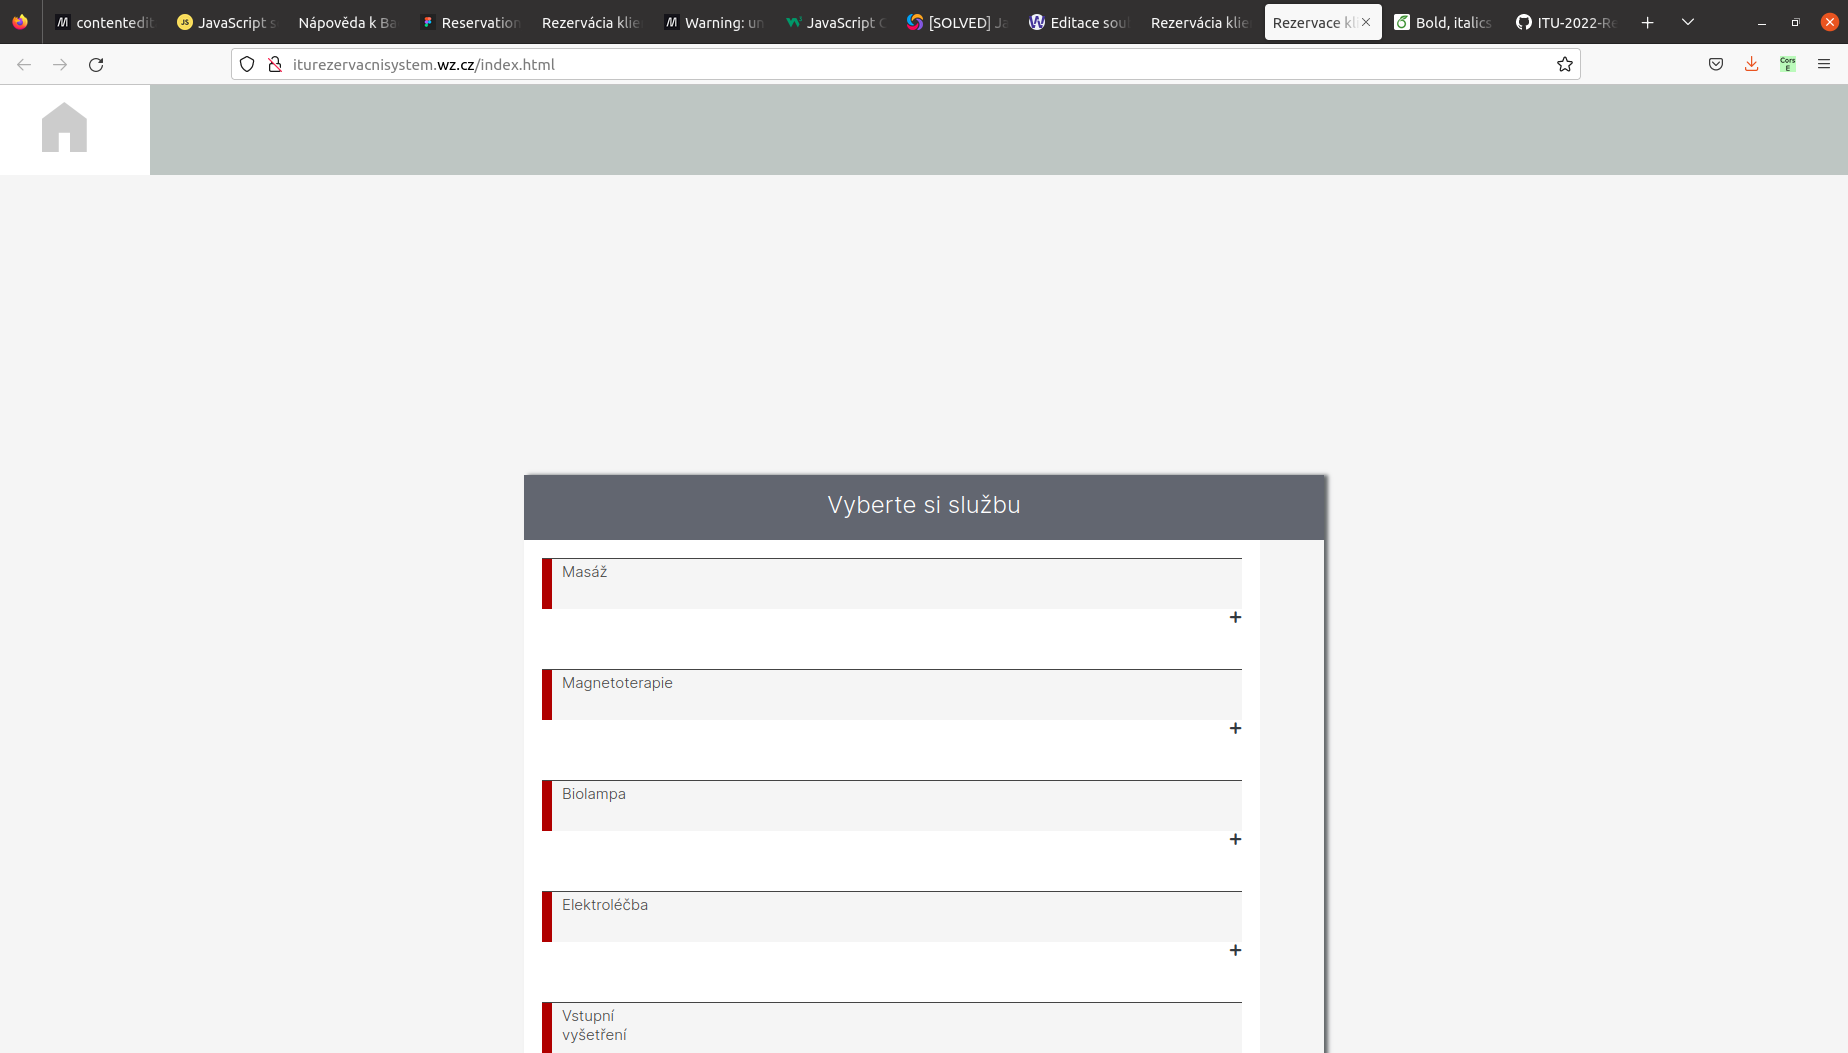
\includegraphics[width=.8\linewidth]{doc/latex/fig/implementation/client/step1.png}
        \caption{}
        \label{fig:step1}
    \end{subfigure}
    \begin{subfigure}{.5\textwidth}
        \centering
        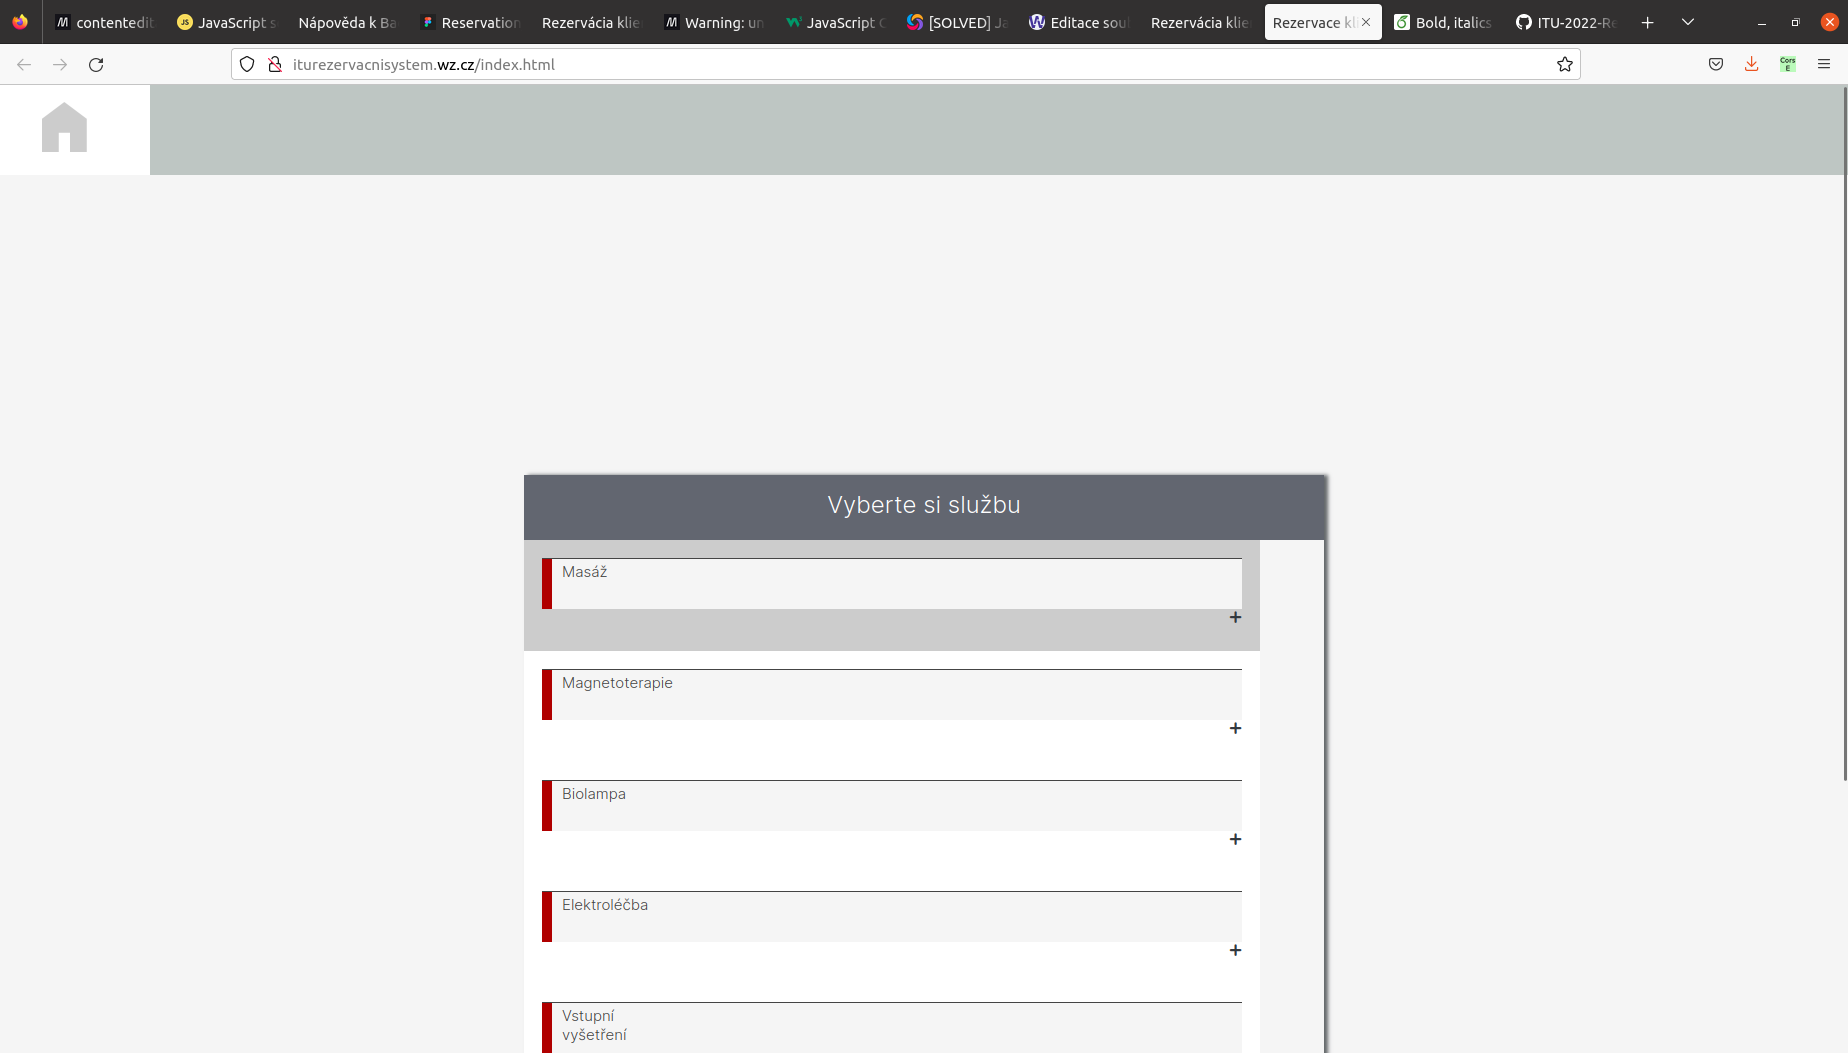
\includegraphics[width=.8\linewidth]{doc/latex/fig/implementation/client/step2.png}
        \label{fig:steps1}
    \end{subfigure}
\end{figure}

\begin{figure}[h]
    \begin{subfigure}{.5\textwidth}
        \centering
        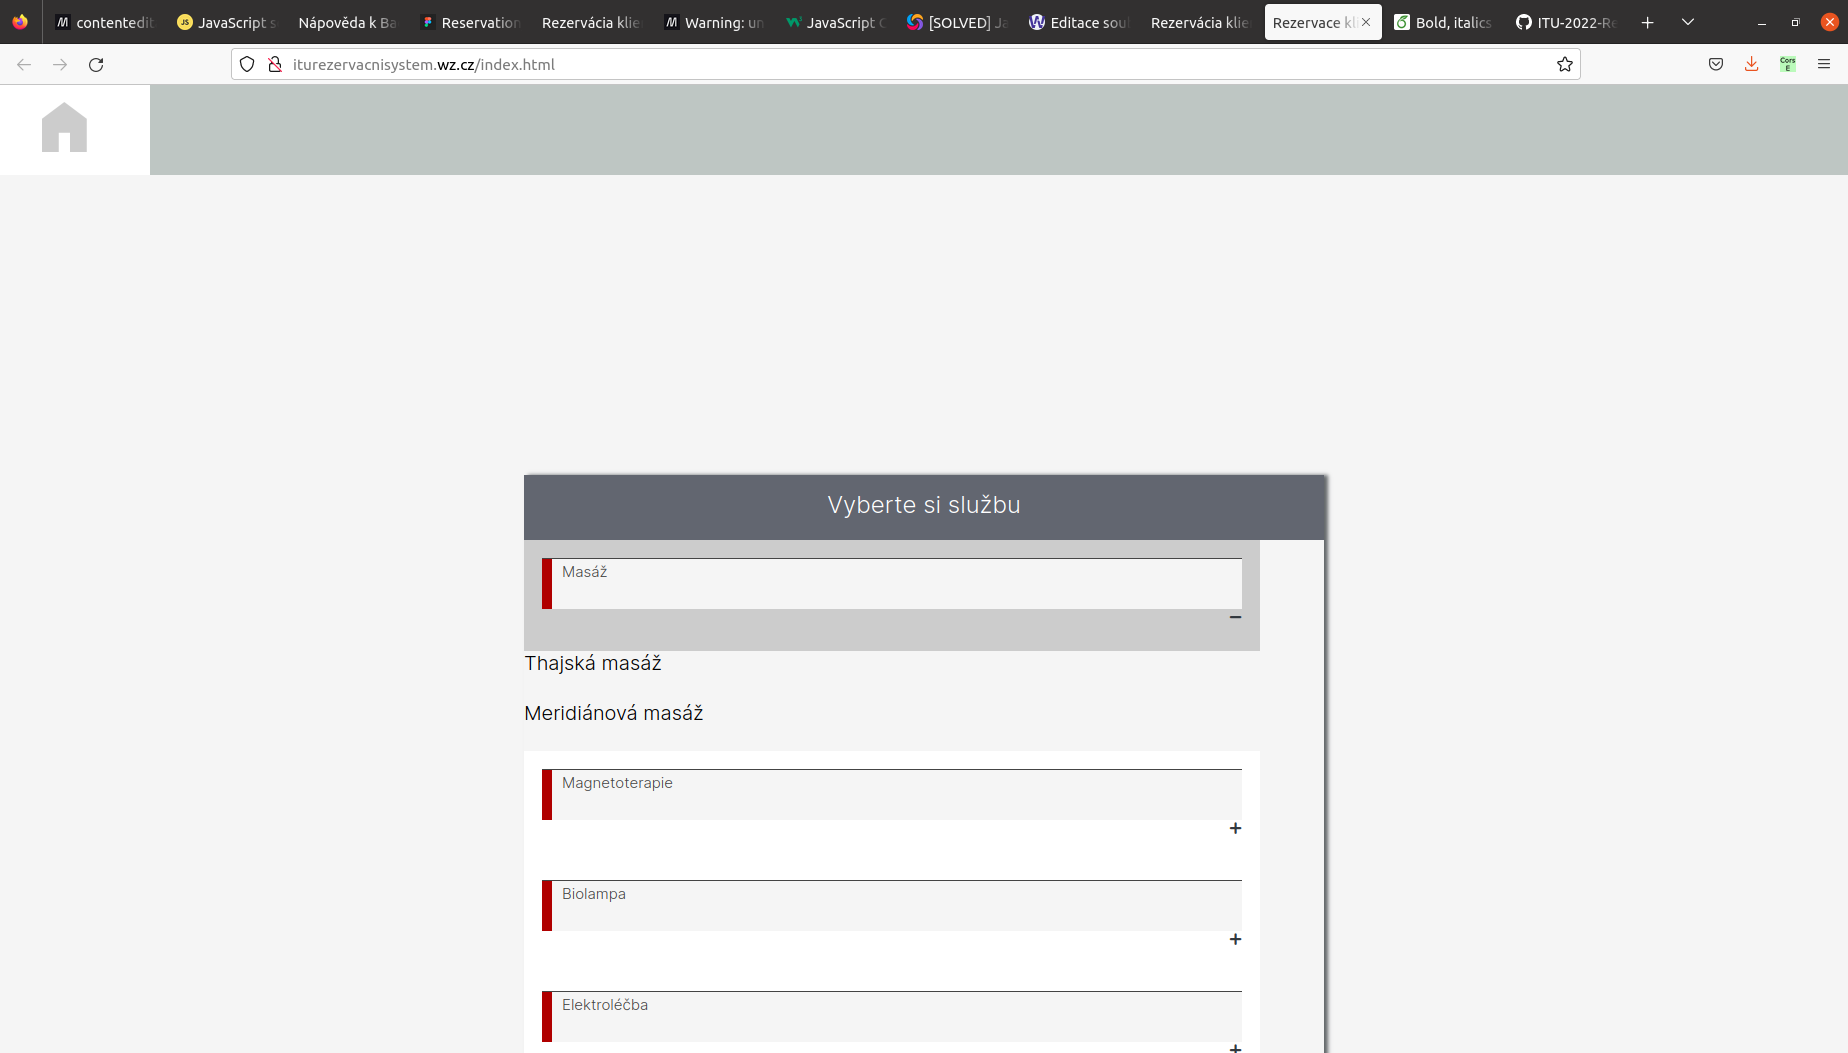
\includegraphics[width=.8\linewidth]{doc/latex/fig/implementation/client/step3.png}
        \caption{}
        \label{fig:step1}
    \end{subfigure}
    \begin{subfigure}{.5\textwidth}
        \centering
        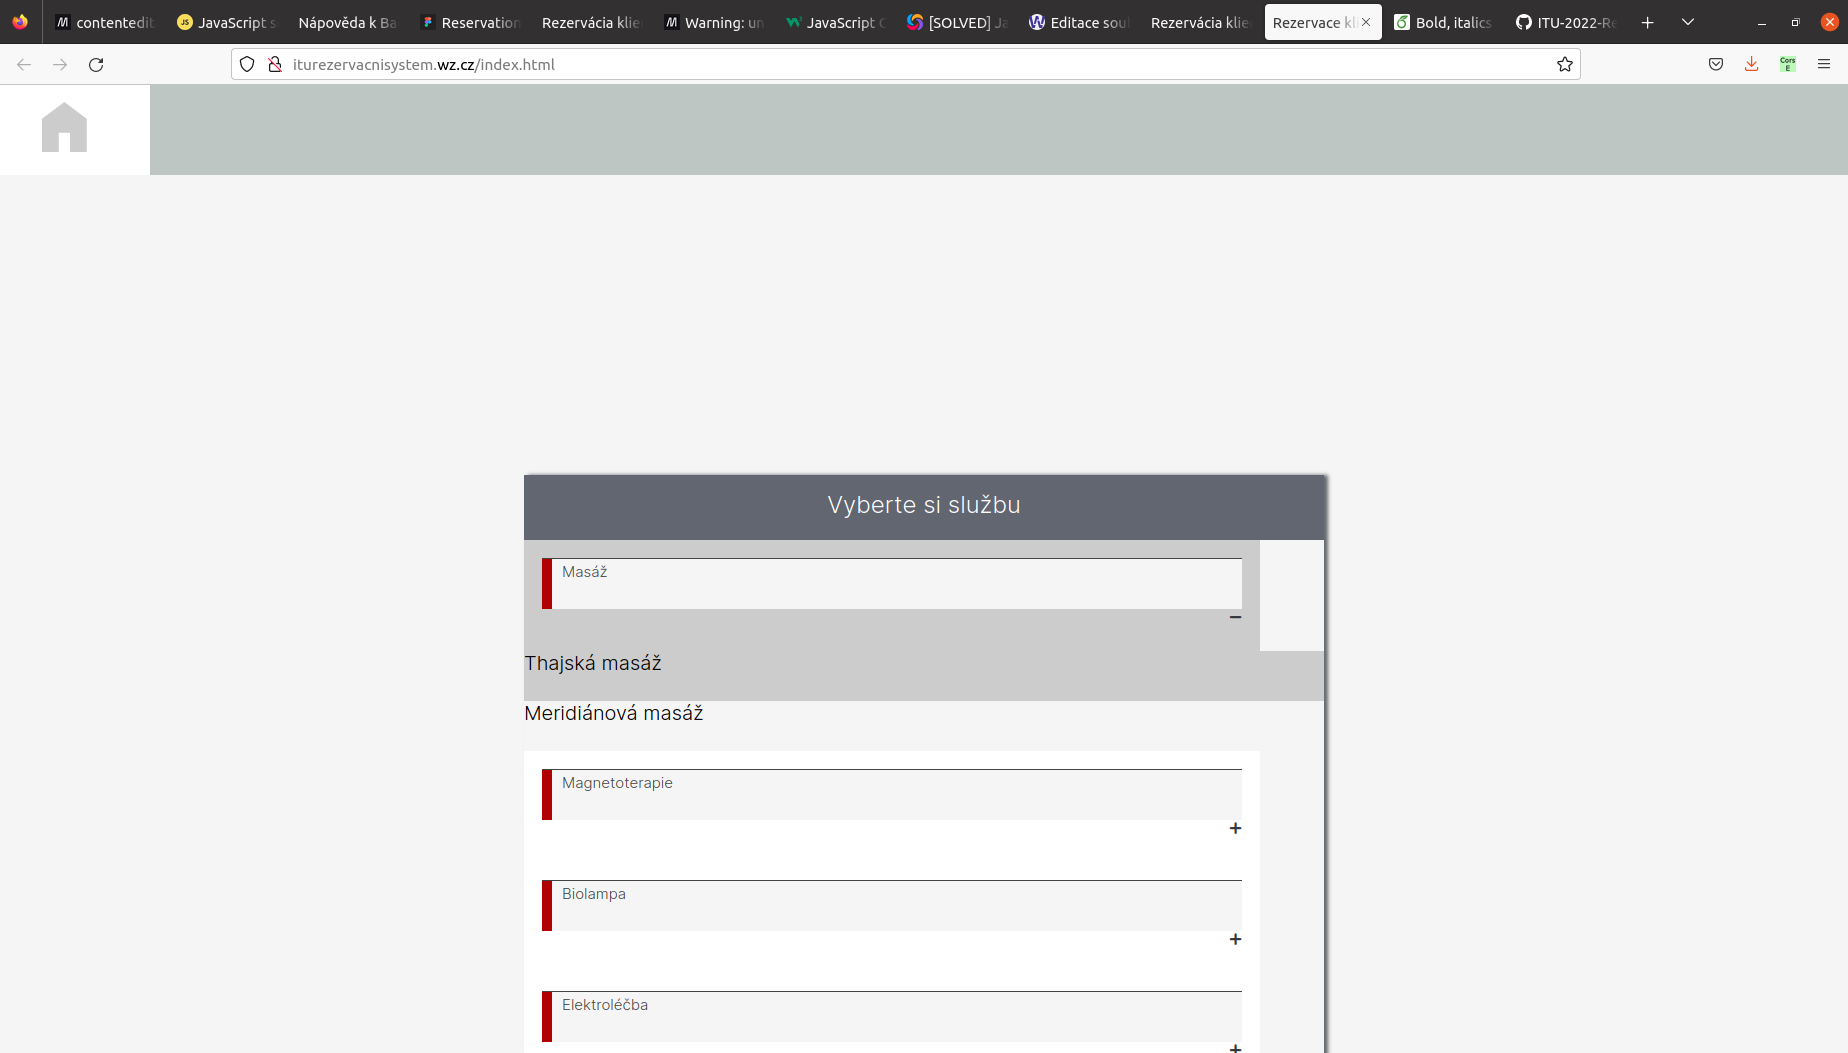
\includegraphics[width=.8\linewidth]{doc/latex/fig/implementation/client/step4.png}
        \caption{}
        \label{fig:step2}
    \end{subfigure}
    \label{fig:steps2}
\end{figure}

\begin{figure}[h]
    \begin{subfigure}{.5\textwidth}
        \centering
        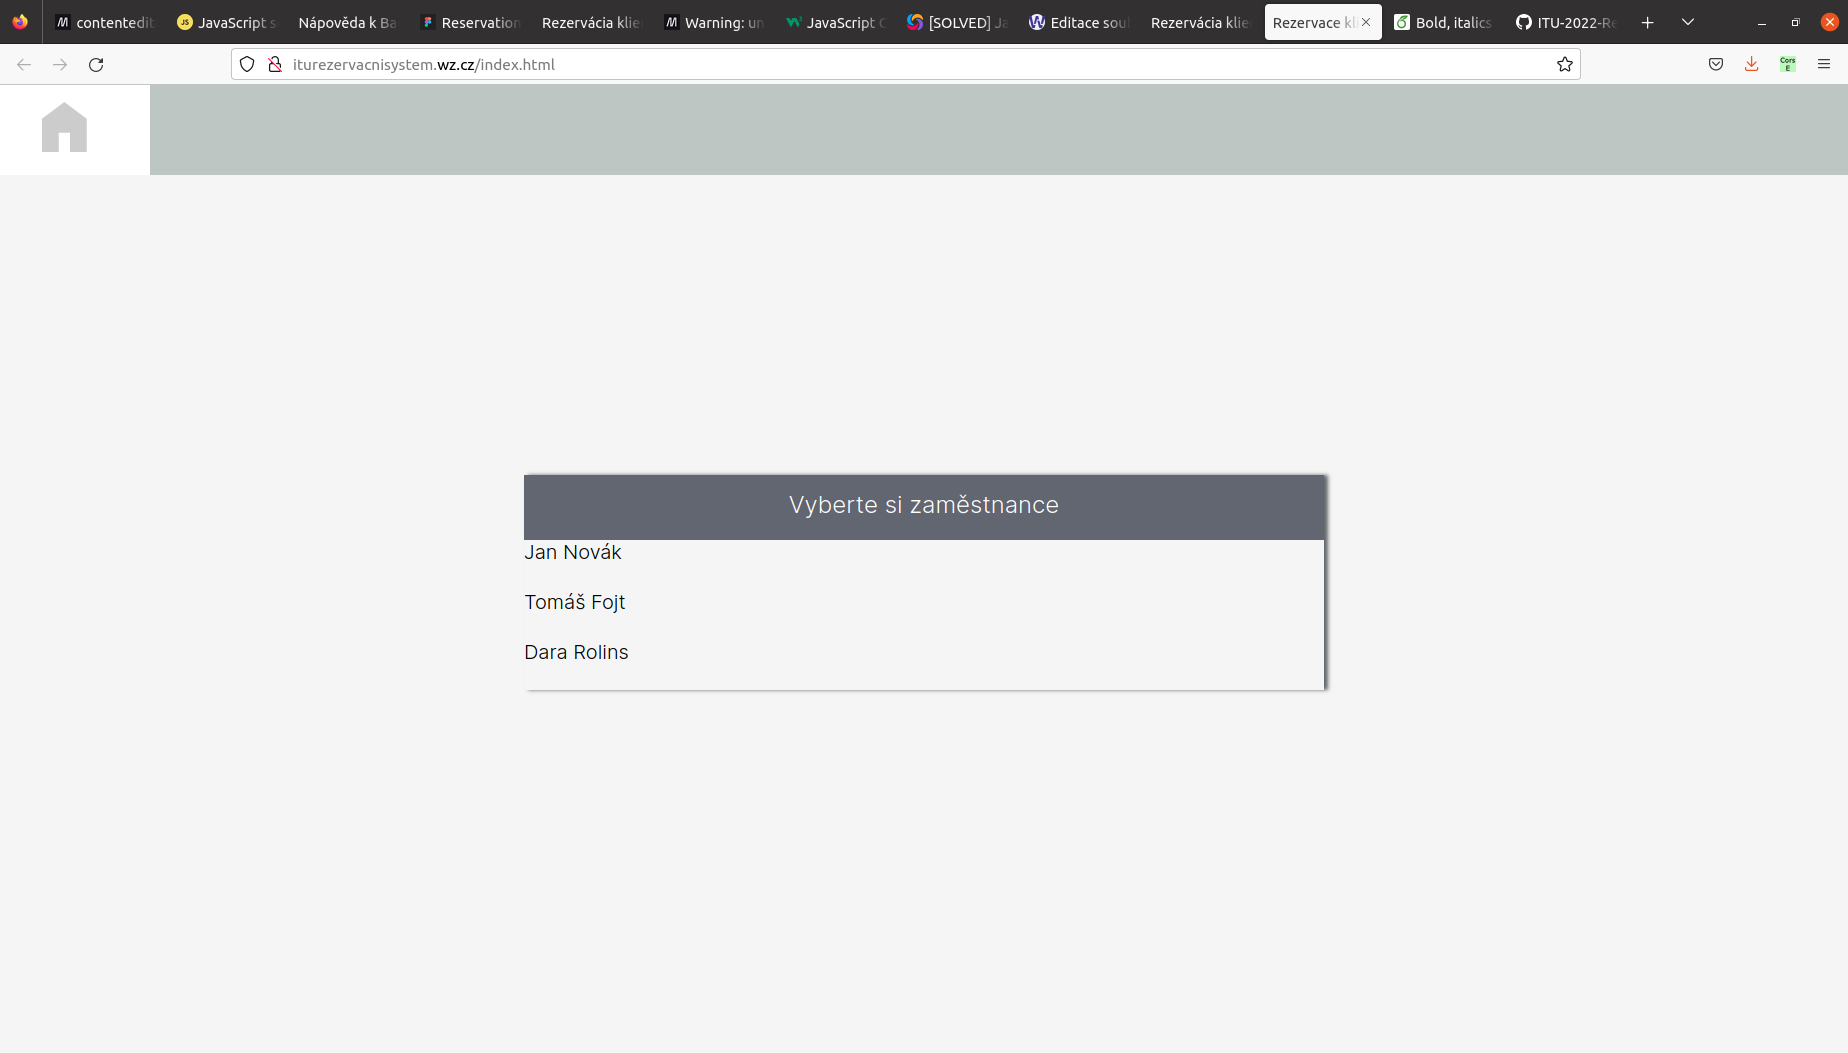
\includegraphics[width=.8\linewidth]{doc/latex/fig/implementation/client/step5.png}
        \caption{}
        \label{fig:step5}
    \end{subfigure}
    \begin{subfigure}{.5\textwidth}
        \centering
        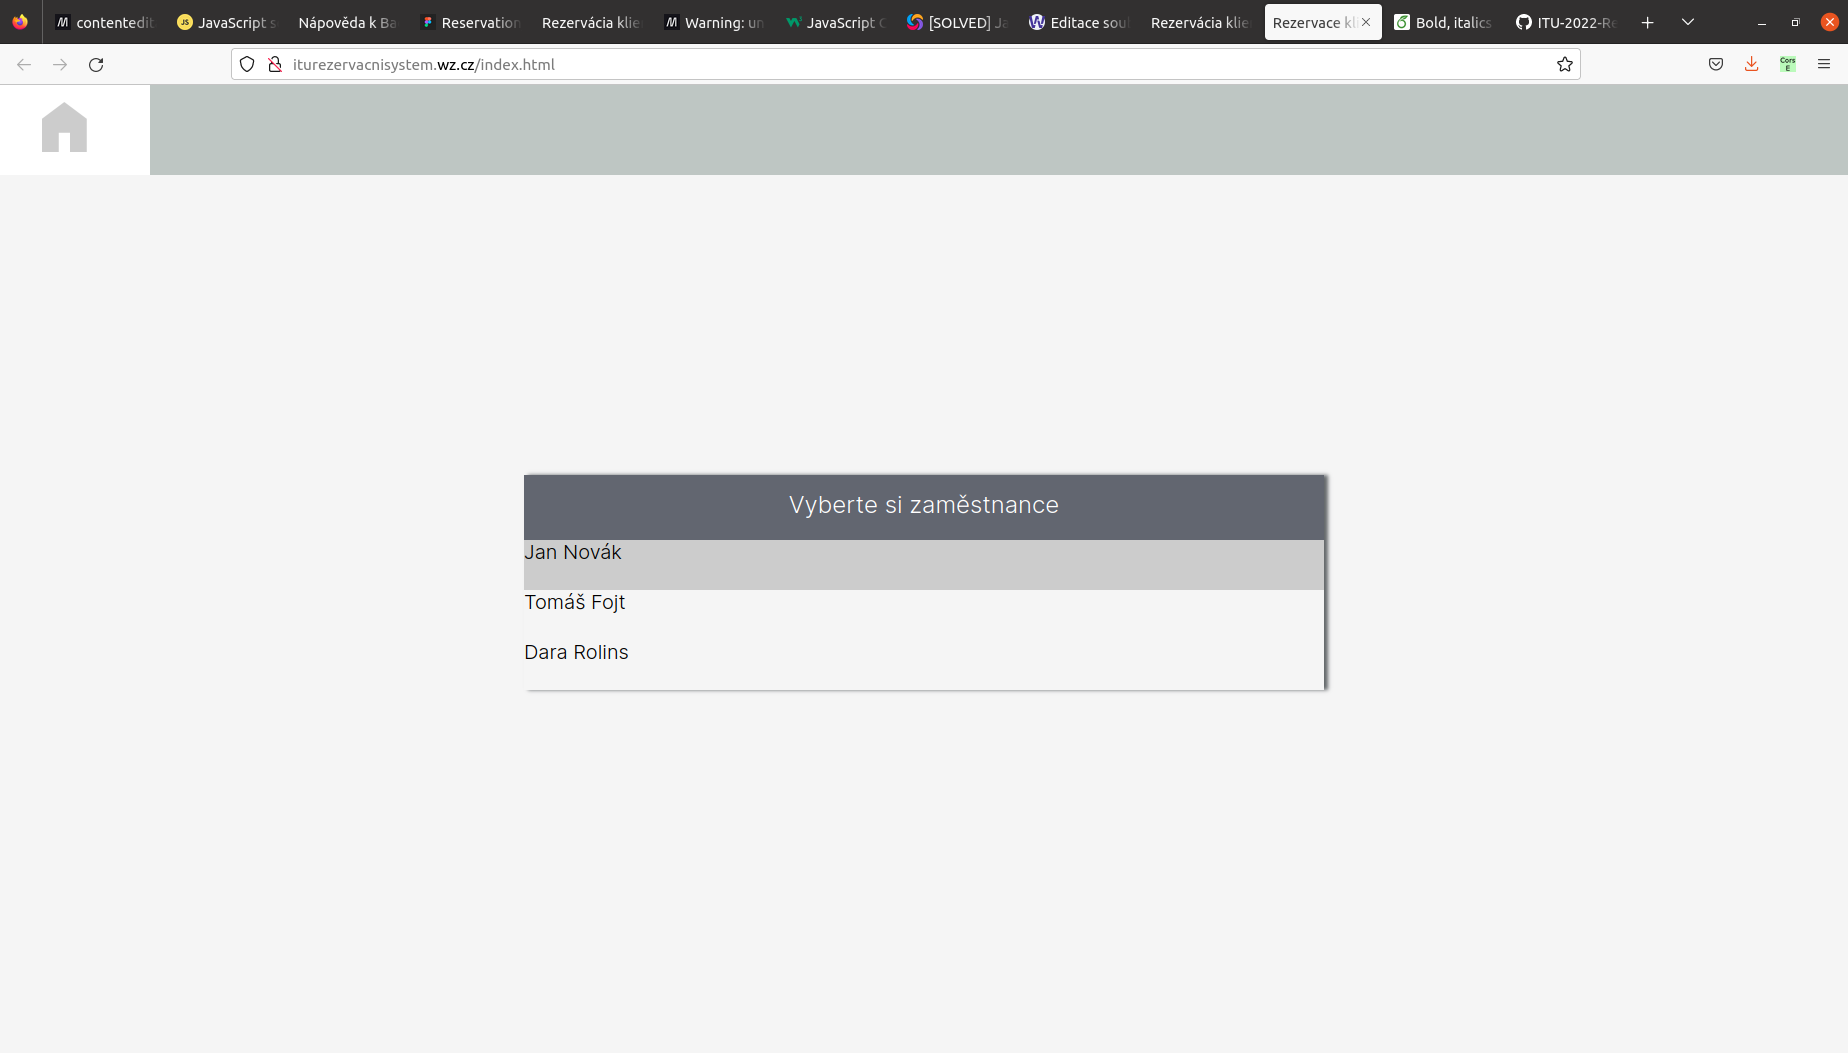
\includegraphics[width=.8\linewidth]{doc/latex/fig/implementation/client/step6.png}
        \caption{}
        \label{fig:step6}
    \end{subfigure}
    \caption{}
    \label{fig:steps3}
\end{figure}

\begin{figure}[h]
    \centering
    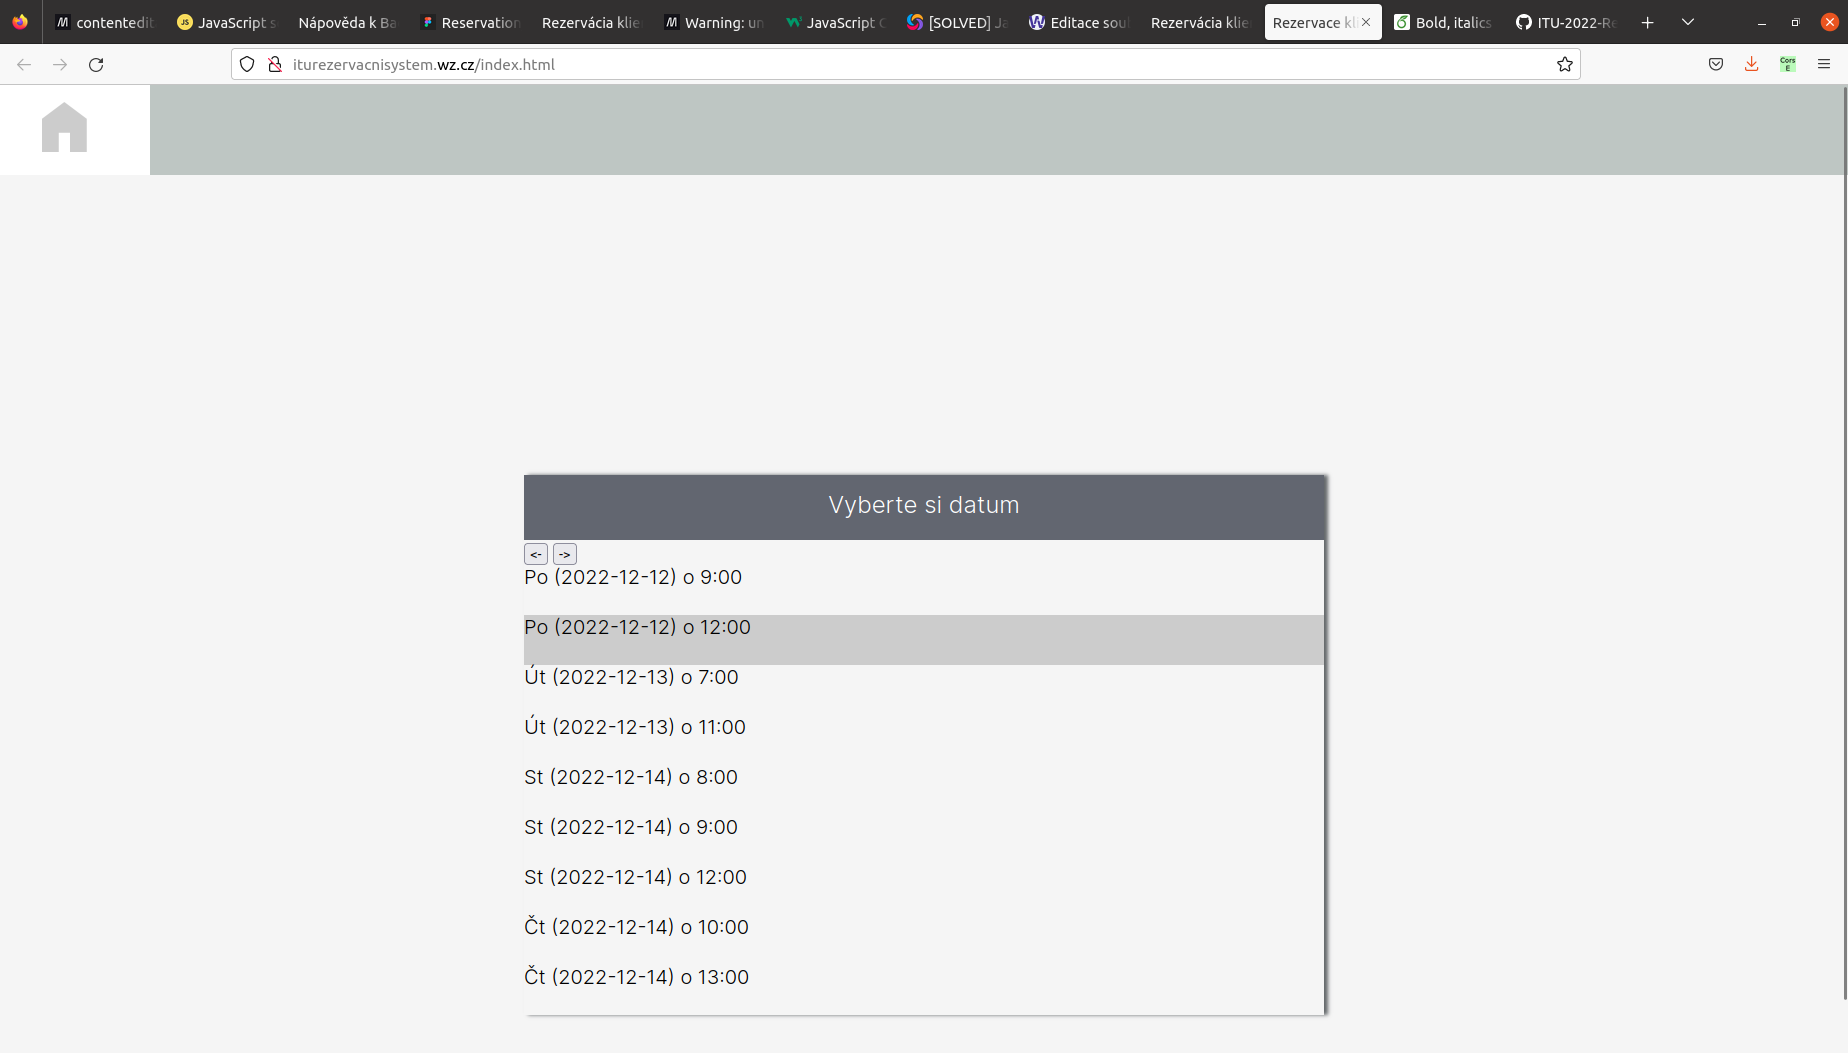
\includegraphics[width=.8\textwidth]{doc/latex/fig/implementation/client/step7.png}
    \caption{}
    \label{fig:step7}
\end{figure}

\newpage

    \section{Implementace}

\subsection*{Konkrétní rozdělení práce v tůmu}
\begin{itemize}
    \item[] Ondřej Fojt     - administrativní pracovník
    \item[] Vít Hrbáček     - Fyzioterapeut
    \item[] Vladimír Mečiar - Pacient
\end{itemize}

\subsection*{Popis použitých nástrojů}
    knihovna JQuery pro jednodušší práci s javascriptem


\subsection*{Popis implementace}

\subsubsection*{Administrativní pracovník}

Celá sekce pro administrativního pracovníka je implementována v rámci jednoho html souboru, ve kterém se schovávají a objevují prvky.
Všechna komunikace s BE je prováděna asynchronně a to funkcí \hyperlink{https://api.jquery.com/jQuery.getJSON/}{jQuery.getJSON( url [, data ] [, success ] )}.

Na všech zobrazeních lze přepínat datum po dnech s výjimkou kalendáře, kde se posouvá po celém týdnu.
Po kliknutí na službu v rámci grafu vytíženosti se zobrazí 2 další grafy pro danou službu. Tyto grafy reprezentují vytíženost zaměstnanců pro danou službu a vytíženost celé služby(všech zaměstnanců) sepsané po dnech(počet následujících dní je omezen pouze počtem vracených dat na BE).
V rámci grafu vytíženosti zaměstnanců a v seznamu zaměstnanců jsou odkazy na kalendář, kde se zobrazují konkrétní registrace.
Graf vytíženosti mění svůj význam podle výběru, tedy pokud se zvolila konkrétní služba tak se zobrazuje Vytíženost zaměstnanců v rámci služby v jeden den a vytíženost služby po dnech.
Vyhledávání na úvodní stránce by mělo vyhledávat služby, zaměstnance a pacienty, ale je pouze implementované vyhledávání služeb.
V kalendáři se lze po kliknutí na registraci zobrazení její detaily.
Měla by být možnost přidávat a odebírat(potažmo přesunout) registrace, ale toto není implementováno.
Zásobník akcí pro undo, není bohužel implementován, ale tlačítkem domů v levém horním rohu se lze vrátit na počáteční stránku.

Stránky administrativního pracovníka lze prohlížet \hyperlink{https://www.stud.fit.vutbr.cz/~xfojto00/ITU/adm_wkr/}{zde}.


\subsubsection*{Fyzioterapeut}

Rozhraní určené pro pracovníky Fyzioterapeutického oddělení, fyzioterapeuty, bylo vytvořeno v oddělené a současně samostatné jednotce 
HTML souboru, ind.html. Kód byl sestaven z prvků v jazycích HTML, CSS a JavaScript. Prvek HTML tabulky byl využit pro tvorbu rozvrhu, 
CSS šablona je určena například k tomu,  aby jednotlivé prvky dala na jejich pozice nebo zajišťuje, že každý sudý sloupec tabulky má jinou barvu.
Sekce JavaScriptového kódu slouží k načtení dat z backendu pro splnění podle pravidel pro MVC. Program kontroluje každé dvě sekundy zda se rozvrh 
nezměnil. Dvě sekundy jsme v týmu zvolili jako rozumnou dobu, kdy nemusí uživatel moc čekat, ale současně zároveň má velmi aktuální rozvrh. 
Pro zajištění komunikace s daty v backendové části jsme použili asynchronní komunikaci stejnou jako byla na cvičení.

Stránky fyzioterapeuta lze prohlížet \hyperlink{http://iturezervacnisystem.wz.cz/ind.html}{zde}.

\subsubsection*{Pacient}


\section*{Výsledná aplikace}

\subsection{Administrativní pracovník}

\begin{figure}[htbp]
    \centering
    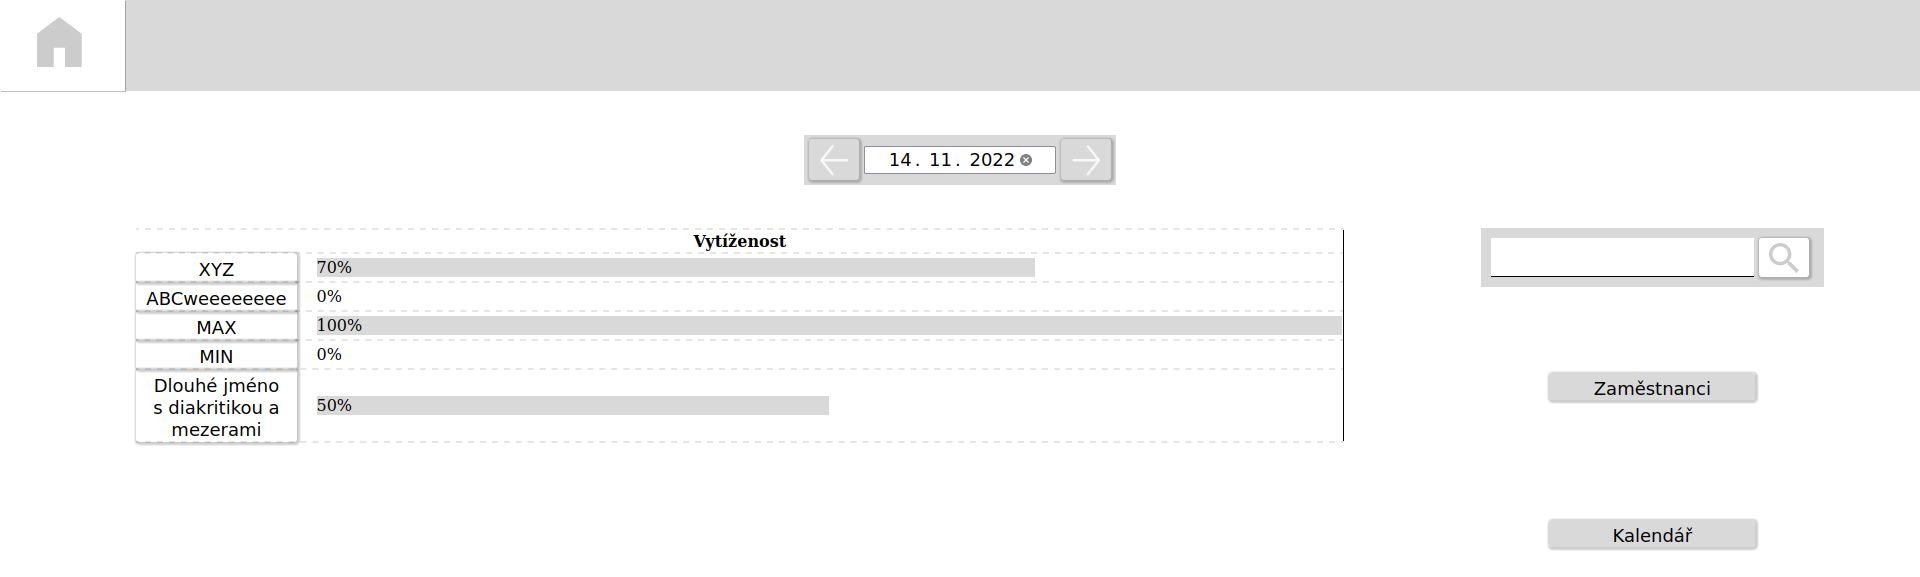
\includegraphics[angle=0, origin=c, width = \textwidth]{doc/latex/fig/implementation/admin/main_page.png}
    \caption{Hlavní stránka administrativního pracovníka}
\end{figure}

\begin{figure}[htbp]
    \centering
    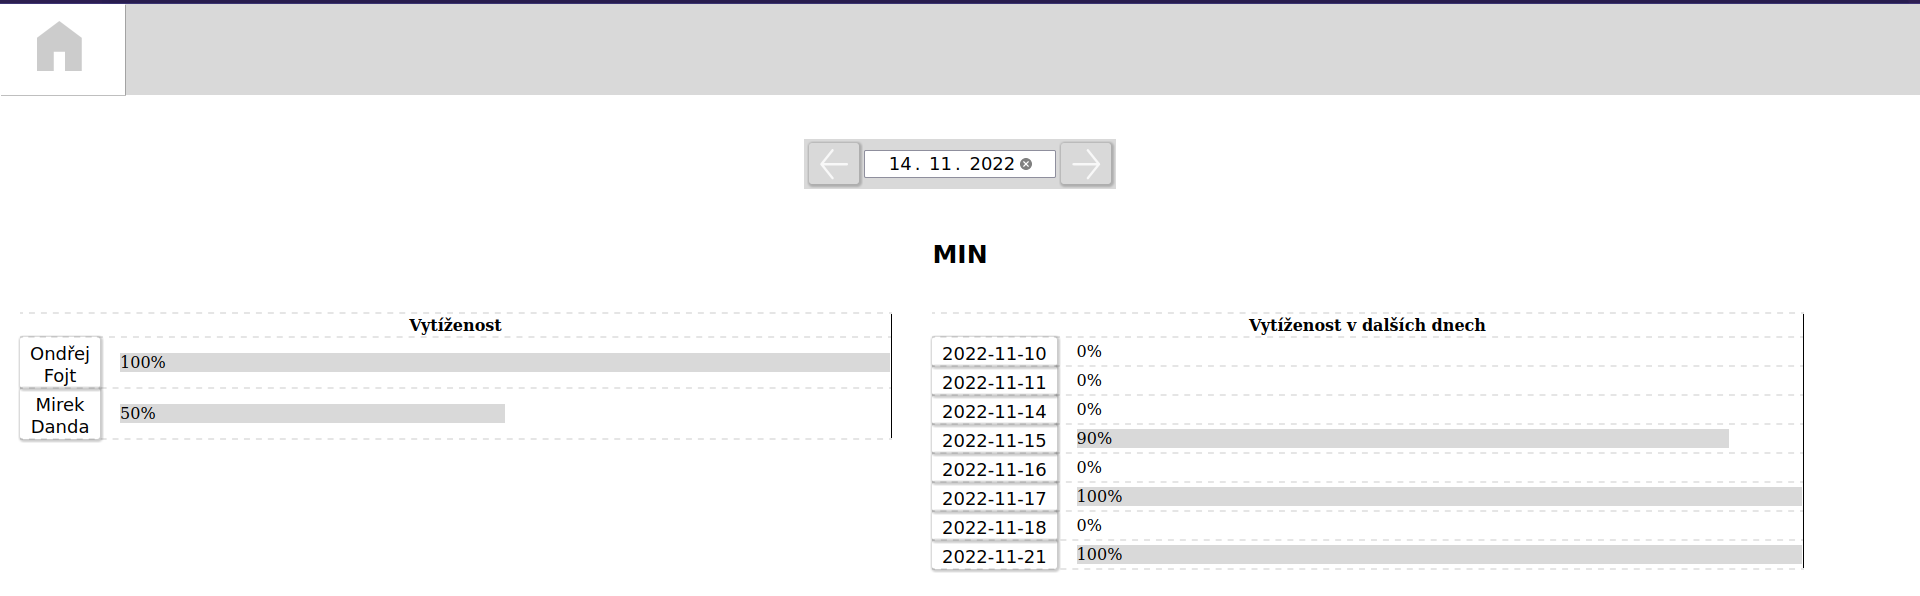
\includegraphics[angle=0, origin=c, width = \textwidth]{doc/latex/fig/implementation/admin/service.png}
    \caption{Grafy zaplněnosti pro danou službu}
\end{figure}

\begin{figure}[htbp]
    \centering
    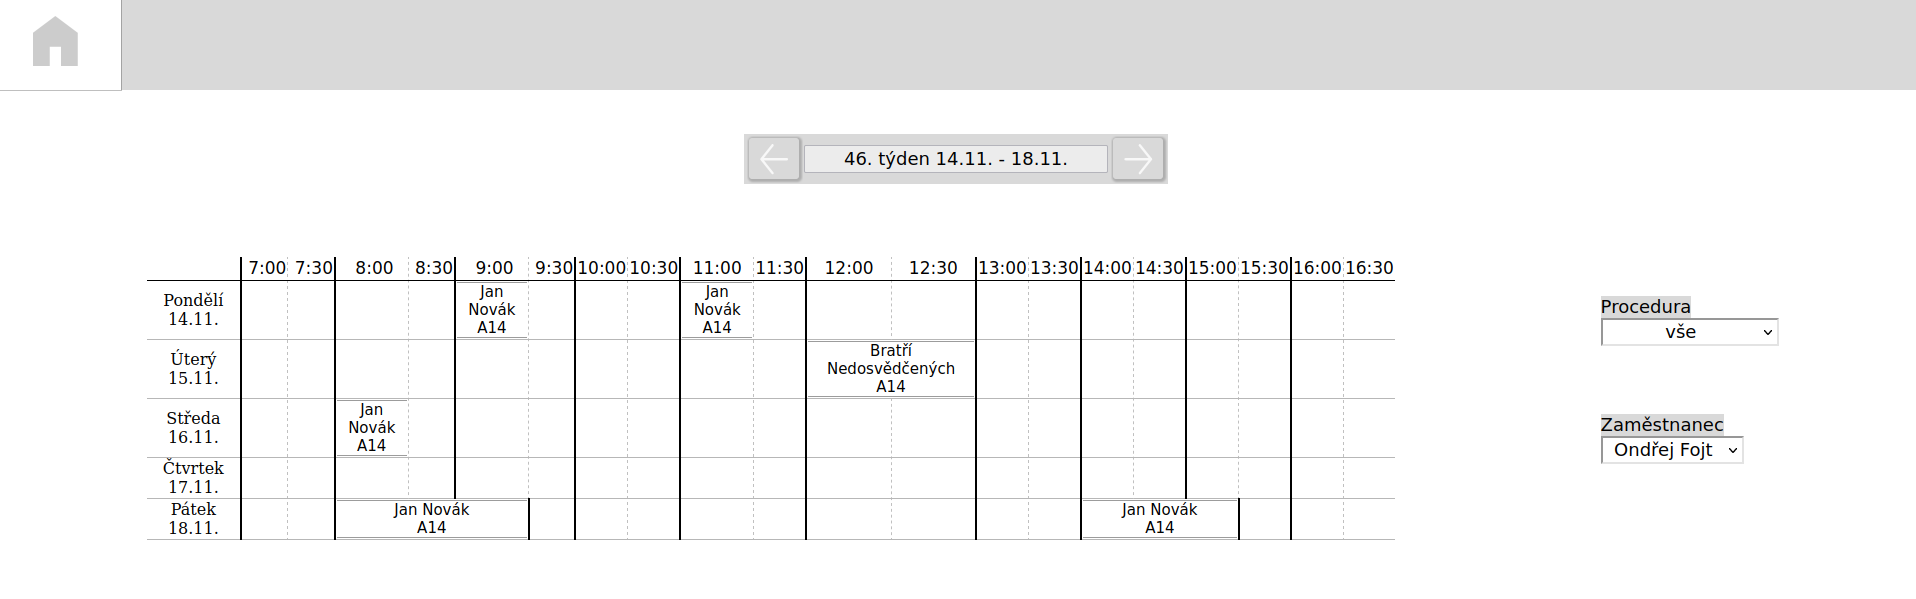
\includegraphics[angle=0, origin=c, width = \textwidth]{doc/latex/fig/implementation/admin/calendar.png}
    \caption{Kalendář služeb/procedur}
\end{figure}



\begin{figure}[htbp]
    \centering
    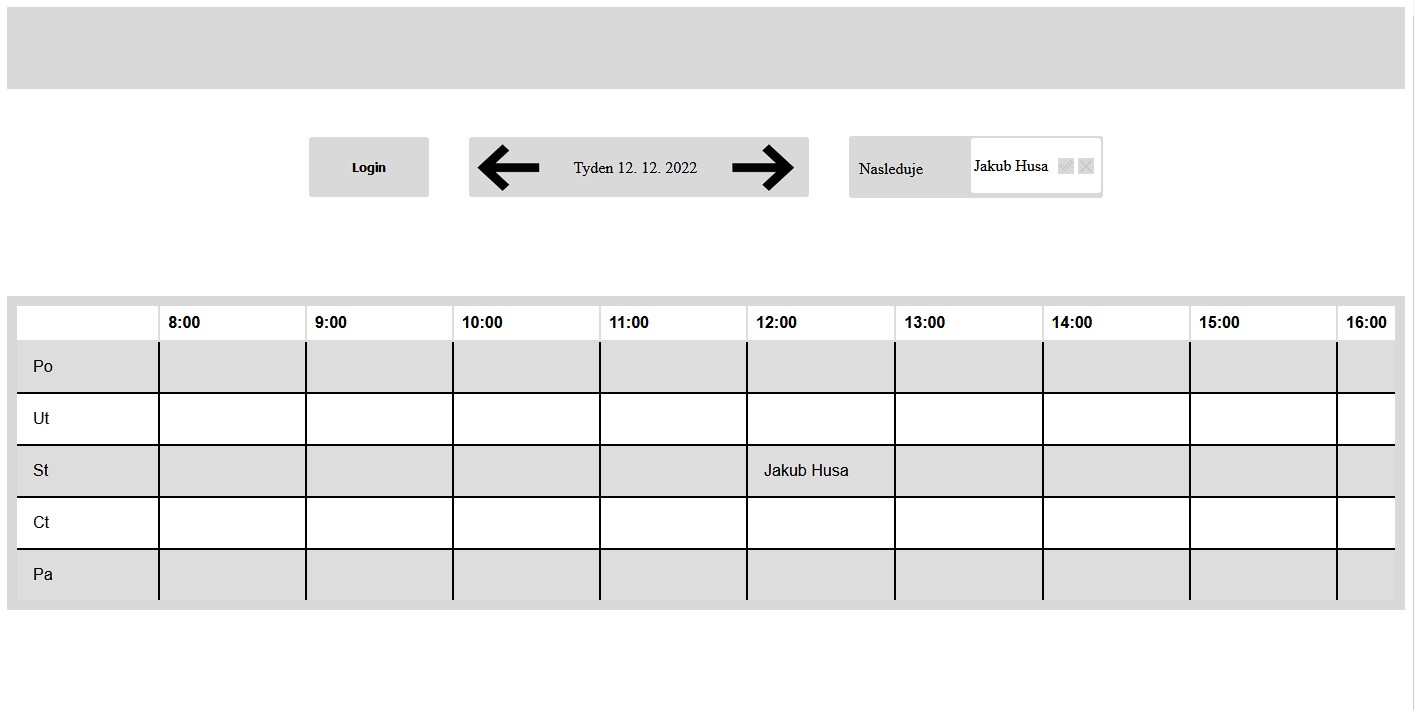
\includegraphics[angle=0, origin=c, width = \textwidth]{doc/latex/fig/implementation/fyzio/printscreen_fyzio.jpg}
    \caption{Stránka fyzioterapeuta}
\end{figure}

    \section{Testování}
Každý z členů si našel minimálně dva kandidáty, které odpovídali jeho minimálním požadavkům na otestování softwaru a následně nám pomohli zkusit otestovat intuitivnost našeho zpracování projektu.

\subsection{Administrativní pracovník}

Testování stránky administrativního pracovníka probíhalo na starší úřední osobě.
Bylo testováno, zda lze najít konkrétní záznam, aniž by se musel ptát na cestu nebo proklikávat jinými cestami.
Na první pohled byly některé tlačítka poměrně špatně viditelné.
Změna zobrazovaného dne nebyla nijak moc problematická.
Není patrné(nezobrazí se správný kurzor), že na položky v kalendáři lze klikat.
Nepochopení významu vytíženosti zaměstnanců v rámci jedné služby.
\emph{Několik drobných chyb chování. Například: Nezobrazení textu "Všichni" při otevření kalendáře z vytíženosti konkrétní služby, přes kliknutí na den v sloupcovém grafu.}

Sehnali jsme na testování jednu mladší doktorku, která se ochotně zúčastnila. První na domovské stránce se statistikami zatížení dostala za úkol najít rozvrh zaměstnance \emph{Ondřeje Fojta} a ač nikde nebyla hned možnost s nápisem Rozvrh, tak rychle sama od sebe správně zareagovala a klikna na tlačítko \emph{Zaměstnanci} z kterého se nakonec dostala k rozvrhu daného zaměstnance. Sice měla testující vnitřní pocit nejistoty a snažila se ujistit, zda to nedělá špatně, ale i bez odpovědi to zvládla najít sama. 
Dalším úkol bylo najít vytíženost jedné konkrétní služby. Jednoduše se z rozvrhu zvládla vrátit na domovskou stránku a najít konkrétní službu a oznámit její vytíženost. 
Poslední úkol byl najít detailní informace o rezervacích. Testující zašla do kalendáře, našla si rezervaci a zjistila všechny potřebné údaje. Celkově ohodnotila práci se službou kladně až na mírné technické problémy po kliknutí na prázdné políčko rozvrhu. 

Tlačítko domů nejde dobře vidět a je hodně zřejmá absence možnosti kroku zpět.
U zobrazování Vytíženosti služeb v následující dny nedává smysl zobrazovat také dny předchozí.
Popisky s nápovědou, co která akce udělá/ukáže.

\subsection{Fyzioterapeut}
Testování rozhraní pro fyzioterapeuta proběhlo na dvou osobách. První byla osoba v pokročilejším věku. Přes svůj věk má několik zkušeností s počítači. Testování proběhlo zadáváním cílů, kde si osoba, která testovala musela sama poradit, jak software k dosažení využít. Např. první osoba bylo za úkol zadáno najít v rozvrhu konkrétního pacienta v některém z nespecifikovaných následujících týdnů. Překvapivě si vůbec první osoba nevšimla šipek a myslela si, že políčko s následující osobou je vyhledávání. Nakonec na to přišla a našla daného pacienta.

Druhá mladší dospělá osoba, která testovala stejný úkol ho zvládla bez problému v překvapivě krátkém čase a stejně tak, všechny další alternativy zadání.
 
Metrikem bylo jednoznačně primárně očekávání, jak bude rozhraní použito, které se částečně splnilo. Zklamáním byl výsledek první starší osoby, ale díky němu přišli náměty na vylepšení. Např. přidání vyhledávání a mírnou změnu vzhledu položky následuje, aby tak nepřipomínala vyhledávání. 

\subsection{Pacient}
viz sekce \ref{client_testing}

    
    \section{Použitá literatura}
    Při implementaci byla použita literatura z webů Blog Hubspot, \hyperlink{https://www.w3schools.com/js/js_arrays.asp}{W3.com}, \hyperlink{https://www.jakpsatweb.cz/javascript/objekt-date.html}{JakPsatWeb.cz}, \hyperlink{https://stackoverflow.com/questions/7755088/what-does-href-expression-a-href-javascript-a-do}{StackOverflow}, \hyperlink{https://www.interval.cz/clanky/promenne-v-javascriptu/}{Interval.cz}, \hyperlink{https://www.youtube.com/playlist?list=PLillGF-RfqbYJVXBgZ_nA7FTAAEpp_IAc}{YouTube} a další.

\end{document}
